%% ----------------------------------------------------------------
%% Thesis.tex -- MAIN FILE (the one that you compile with LaTeX)
%% ---------------------------------------------------------------- 

% Set up the document
\documentclass[a4paper, 11pt, oneside]{Thesis}  % Use the "Thesis" style, based on the ECS Thesis style by Steve Gunn
\graphicspath{Figures/}  % Location of the graphics files (set up for graphics to be in PDF format)

% Include any extra LaTeX packages required
\usepackage[square, numbers, comma, sort&compress]{natbib}  % Use the "Natbib" style for the references in the Bibliography
\usepackage[utf8]{inputenc}
\usepackage{vntex} % Vietnamese Typeset for Latex
\usepackage{tikz}
\usepackage{tikz-qtree}
\usepackage{multicol}
\usepackage{multirow}
\usepackage{hyperref}
\usepackage{graphicx}
\usepackage{float}
\usepackage{pifont}% http://ctan.org/pkg/pifont
\newcommand{\cmark}{\ding{51}}%
\newcommand{\xmark}{\ding{55}}%
\usepackage{verbatim}  % Needed for the "comment" environment to make LaTeX comments


\usepackage{fancyvrb}
\usepackage{vector}  % Allows "\bvec{}" and "\buvec{}" for "blackboard" style bold vectors in 
\hypersetup{urlcolor=blue, colorlinks=true}  % Colours hyperlinks in blue, but this can be distracting if there are many links.
%% ----------------------------------------------------------------
%% fill a page with dotlines 
\makeatletter

\newlength\dottedlinefillheight
\setlength\dottedlinefillheight{.25in}


\newcommand\fillwithdottedlines[1]{%
	\begingroup
	\ifhmode
	\par
	\fi
	\hrule height \z@
	\nobreak
	\setbox0=\hbox to \hsize{\hskip \@totalleftmargin
		\vrule height \dottedlinefillheight depth \z@ width \z@
		\dotfill}%
	% We use \cleaders (rather than \leaders) so that a given
	% vertical space will always produce the same number of lines
	% no matter where on the page it happens to start:
	\cleaders \copy0 \vskip #1 \hbox{}%
	\endgroup
}
\makeatother
%% ----------------------------------------------------------------
\begin{document}
\frontmatter      % Begin Roman style (i, ii, iii, iv...) page numbering

% Set up the Title Page
\title  {Khoá luận tốt nghiệp 1-2015}
\supervisor{\texorpdfstring{TS. Nguyễn Anh Tuấn{Supervisor Name}}}
\examiner    {}
\degree      {}
\authors  {\texorpdfstring
            {Chương Đặng - 10520010}{Author Name}
            \\
            \texorpdfstring
            {Duy Nguyễn - 10520011}{Author Name}
            }
\addresses  {\groupname\\\deptname\\\univname}  % Do not change this here, instead these must be set in the "Thesis.cls" file, please look through it instead
\date       {\today}
\subject    {}
\keywords   {}

\maketitle
%% ----------------------------------------------------------------

\setstretch{1.3}  % It is better to have smaller font and larger line spacing than the other way round

% Define the page headers using the FancyHdr package and set up for one-sided printing
\fancyhead{}  % Clears all page headers and footers
\rhead{\thepage}  % Sets the right side header to show the page number
\lhead{}  % Clears the left side page header

\pagestyle{fancy}  % Finally, use the "fancy" page style to implement the FancyHdr headers

%% ----------------------------------------------------------------
% Declaration Page required for the Thesis, your institution may give you a different text to place here
%\Declaration{
%
%\addtocontents{toc}{\vspace{1em}}  % Add a gap in the Contents, for aesthetics
%
%I, AUTHOR NAME, declare that this thesis titled, `THESIS TITLE' and the work presented in it are my own. I confirm that:
%
%\begin{itemize} 
%\item[\tiny{$\blacksquare$}] This work was done wholly or mainly while in candidature for a research degree at this University.
% 
%\item[\tiny{$\blacksquare$}] Where any part of this thesis has previously been submitted for a degree or any other qualification at this University or any other institution, this has been clearly stated.
% 
%\item[\tiny{$\blacksquare$}] Where I have consulted the published work of others, this is always clearly attributed.
% 
%\item[\tiny{$\blacksquare$}] Where I have quoted from the work of others, the source is always given. With the exception of such quotations, this thesis is entirely my own work.
% 
%\item[\tiny{$\blacksquare$}] I have acknowledged all main sources of help.
% 
%\item[\tiny{$\blacksquare$}] Where the thesis is based on work done by myself jointly with others, I have made clear exactly what was done by others and what I have contributed myself.
%\\
%\end{itemize}
% 
% 
%Signed:\\
%\rule[1em]{25em}{0.5pt}  % This prints a line for the signature
% 
%Date:\\
%\rule[1em]{25em}{0.5pt}  % This prints a line to write the date
%}
%\clearpage  % Declaration ended, now start a new page

%% ----------------------------------------------------------------
% The "Funny Quote Page"
% \pagestyle{empty}  % No headers or footers for the following pages

% \null\vfill
% Now comes the "Funny Quote", written in italics
% \textit{``Write a funny quote here.''}

% \begin{flushright}
% If the quote is taken from someone, their name goes here
% \end{flushright}

% \vfill\vfill\vfill\vfill\vfill\vfill\null
% \clearpage  % Funny Quote page ended, start a new page
%% ----------------------------------------------------------------

% The Abstract Page

%\addtotoc{Lời mở đầu}  % Add the "Abstract" page entry to the Contents
%\abstract{
%\addtocontents{toc}{\vspace{1em}}  % Add a gap in the Contents, for aesthetics
%
%\begin{center}{\huge{\textit{
%				Lời mở đầu
%			}} \par}\end{center}
%
%\ldots
%}

\clearpage  
% Abstract ended, start a new page
% -----------------------------------------------------------------
% Opening words
\openingwords{
	\addtocontents{toc}{\vspace{1em}}
Thế giới của chúng ta đang liên tục vận động theo chiều hướng tích cực. Đây là nguyên nhân chủ yếu cho sự phát triển và thay đổi hằng ngày của mọi lĩnh vực đời sống, đặc biệt là khoa học công nghệ nói chung, và ngành công nghệ thông tin nói riêng. Hiện nay, hầu hết mọi nơi trên thế giới đều đã biết đến sự có mặt của công nghệ thông tin, máy tính, và kể cả internet. Việc internet ra đời là một sự kiện đã làm thay đổi cả thế giới. Thay thế cho việc gọi điện thoại hằng ngày, chúng ta có thể liên lạc qua internet, với việc có thể thấy được hình ảnh của người đối diện chứ không chỉ riêng giọng nói. Thay thế cho những tờ báo bằng giấy, chúng ta đã có những trang web, với những thông tin đầy đủ hơn, hình ảnh sinh động hơn, và cả những đoạn video minh hoạ. Những thông tin trên internet được lan truyền với tốc độ chóng mặt, dẫn đến việc những tin tức nóng nhất được cập nhật liên tục trong từng phút từng giây. Cách tiếp cận thông tin của con người thay đổi, nên sự chuyển động của thông tin ngày càng nhanh hơn, và đến mức nào đó, thông tin sẽ không mang theo đủ những gì mà con người mong muốn truyền tải. Đó là lúc mà con người nghĩ đến việc thay đổi. Và đó cũng chính là lúc Semantic Web được ra đời.
\\
Semantic Web mang sứ mệnh lớn lao trong việc thay đổi công nghệ web. Trước đây, máy tính chỉ đóng vai trò là trung tâm “chứa đựng” và “duy trì” các trang web. Tuy nhiên, với Semantic Web, máy tính sẽ phải làm nhiều hơn thế, sẽ phải “suy nghĩ” và “sử dụng” trang web một phần nào đó thay thế cho con người. Để làm được điều này không phải dễ dàng, vì máy tính là vật vô tri vô giác. Do đó, một cách tiếp cận đơn giản để giải quyết vấn đề này, bằng cách thêm vào các trang web thông thường metadata, để các máy tính có thể “đọc” được, như một ngôn ngữđầuung của các máy tính. 
\\
Nhận thấy được những tiềm năng và những lợi ích to lớn của Semantic Web, chúng em đã lựa chọn đề tài này, để nghiên cứu và tìm hiểu sâu hơn về Semantic Web, góp phần đem những kiến thức tìm hiểu được xây dựng thành một luận văn mang tính đóng góp cao. Trong quá trình nghiên cứu, tuy gặp phải những khái niệm và công nghệ hoàn toàn mới lạ và ít được công bố, chúng em vẫn cố gắng tìm hiểu bằng mọi cách. Lĩnh vực Semantic Web là rất rộng lớn, với một khoảng thời gian có hạn, chúng em chỉ có thể tìm hiểu được những vấn đề được coi là cơ bản và tất yếu nhất của Semantic Web. Dù vậy, chúng em rất hài lòng và tự tin với những gì tìm hiểu và nghiên cứu được sẽ mang lại nhiều lợi ích, đóng góp vào công cuộc nghiên cứu khoa học chung.	
} 
\clearpage
% opening words ended, start a new page
%% ----------------------------------------------------------------
\setstretch{1.3}  % Reset the line-spacing to 1.3 for body text (if it has changed)

% The Acknowledgements page, for thanking everyone
\acknowledgements{
\addtocontents{toc}{\vspace{1em}}  % Add a gap in the Contents, for aesthetics

Đầu tiên, chúng em xin chân thành cám ơn Khoa Mạng máy tính và Truyền thông, trường Đại Học Công Nghệ Thông Tin, Đại Học Quốc Gia TP.HCM đã tạo điều kiện cho chúng em hoàn thành tốt khoá luận này.
\\
Chúng em xin chân thành cám ơn Thầy Nguyễn Anh Tuấn, đã tận tình hướng dẫn, dạy dỗ, chỉ bảo chúng em từ những ngày đầu định hình khoá luận cho đến khi hoàn thành. Nhờ sự tận tình của thầy, chúng em đã hoàn thành tốt khoá luận này, bên cạnh đó cũng học hỏi được nhiều kiến thức quý báu từ thầy.
\\
Chúng em xin chân thành cảm ơn quý Thầy Cô trong Khoa Mạng máy tính và truyền thông, trong những năm qua đã không quản ngại mệt mỏi, tận tình giảng dạy, trang bị cho chúng em những kiến thức cần thiết để hoàn thành khoá luận.
\\
Chúng em xin ghi nhớ công ơn sinh thành dưỡng dục của cha mẹ, sự giúp đỡ của các anh, chị, bạn bè trong những năm học, cũng như sự an ủi, động viên trong những lúc khó khăn, vất vả. Dù chúng em đã dùng tất cả nỗ lực của bản thân để hoàn thành tốt khoá luận này, tuy nhiên không thể tránh khỏi những sai sót, thiếu sót, kính mong quý Thầy Cô tận tình chỉ bảo. Một lần nữa, chúng em xin chân thành cảm ơn và mong nhận được nhiều tình cảm chân thành của tất cả mọi người.
\begin{flushright}
Thành phố Hồ Chí Minh, ngày ... tháng ... năm 2015
\\
Sinh viên thực hiện khoá luận	
\\
Đặng Lê Bảo Chương và Nguyễn Bảo Duy
\end{flushright}
% your project advisor\ldots

}
\clearpage  % End of the Acknowledgements
%% ----------------------------------------------------------------
% Nhận xét của giáo viên hướng dẫn
\nhanxetcuagvhd{
\addtocontents{toc}{\vspace{1em}} 
\fillwithdottedlines{20cm}
}
\clearpage
%% ----------------------------------------------------------------
% Nhận xét của giáo viên phản biện
\nhanxetcuagvphanbien{
\addtocontents{toc}{\vspace{1em}} 
\fillwithdottedlines{20cm}
}
\clearpage
%% ----------------------------------------------------------------

\pagestyle{fancy}  %The page style headers have been "empty" all this time, now use the "fancy" headers as defined before to bring them back
%% ----------------------------------------------------------------
\lhead{\emph{Mục lục}}  % Set the left side page header to "Contents"
\tableofcontents  % Write out the Table of Contents

\lhead{\emph{Danh sách hình vẽ}}  % Set the left side page header to "List of Figures"
\listoffigures  % Write out the List of Figures

%% ----------------------------------------------------------------
\lhead{\emph{Danh sách các bảng}}  % Set the left side page header to "List of Tables"
\listoftables  % Write out the List of Tables

%% ----------------------------------------------------------------
\setstretch{1.5}  % Set the line spacing to 1.5, this makes the following tables easier to read
\clearpage  % Start a new page
\lhead{\emph{Abbreviations}}  % Set the left side page header to "Abbreviations"
\listofsymbols{ll}  % Include a list of Abbreviations (a table of two columns)
{
	% Từ viết tắt 		%
	\textbf{KB} 		& \textbf{K}nowledge \textbf{B}ase\\
	\textbf{KR} 		& \textbf{K}nowledge \textbf{R}epresentation\\
	\textbf{DL} 		& \textbf{D}escription \textbf{L}ogic\\
	\textbf{MUPS} 		& \textbf{M}inimal \textbf{U}nsatisfiability \textbf{P}reserving \textbf{S}ub-TBoxes\\
	\textbf{HST} 		& \textbf{H}itting \textbf{S}et \textbf{T}ree\\
	\textbf{HS} 		& \textbf{H}itting \textbf{S}et
}

%% ----------------------------------------------------------------
%\clearpage  % Start a new page
%\lhead{\emph{Physical Constants}}  % Set the left side page header to "Physical Constants"
%\listofconstants{lrcl}  % Include a list of Physical Constants (a four column table)
%{
%% Constant Name & Symbol & = & Constant Value (with units) \\
%Speed of Light & $c$ & $=$ & $2.997\ 924\ 58\times10^{8}\ \mbox{ms}^{-\mbox{s}}$ (exact)\\
%
%}

%% ----------------------------------------------------------------
\clearpage  %Start a new page
\lhead{\emph{Khóa luận tốt nghiệp 1-2015}}  % Set the left side page header to "Symbols"
\listofnomenclature{lll}  % Include a list of Symbols (a three column table)
{
	% symbol 		% explanation						% giải thích
	$\models$ 		& models of 						& có nghĩa trong (KB)\\
	$\not\models$ 	& not a model  of 					& không có nghĩa trong KB\\
	$\subseteq$ 	& is a subset of 					& là tập con của\\
	$\cap$ 			& intersect 						& giao với\\
	$\neg$ $A$ 		& complement of A of 				& không phải A\\
	$\exists$ $R.E$ & e.g \textit{has} some E 			& \\
	$\forall$ $R.E$ & e.g \textit{has} only E 			& \\
	$\equiv$ 		&  is equivalent to 				& tương đương với \\
	$\emptyset$ 	& empty set 						& tập hợp rỗng \\
	$\in$ 			& is member of	 					& thuộc \\
	$\Leftarrow$ 	& preferred for left implication 	& \\
	$\backslash$ 	& except 							& ngoại trừ \\
	& & \\ % Gap to separate the Roman symbols from the Greek
}

%% ----------------------------------------------------------------
% End of the pre-able, contents and lists of things
% Begin the Dedication page

%\setstretch{1.3}  % Return the line spacing back to 1.3
%
%\pagestyle{empty}  % Page style needs to be empty for this page
%\dedicatory{For/Dedicated to/To my\ldots}
%
%\addtocontents{toc}{\vspace{2em}}  % Add a gap in the Contents, for aesthetics


%% ----------------------------------------------------------------
\mainmatter	  % Begin normal, numeric (1,2,3...) page numbering
\pagestyle{fancy}  % Return the page headers back to the "fancy" style

% Include the chapters of the thesis, as separate files
% Just uncomment the lines as you write the chapters

\chapter {Giới thiệu đề tài}
\section{Tên đề tài}
Trình biên soạn Ontology 
\section{Nội dung và giới hạn đề tài}
\subsection{Nội dung đề tài}
OWL ( Web Ontology Language ) là một dạng ngôn ngữ biểu diễn tri thức. Ngôn ngữ này thường được sử dụng phổ biến trong Semantic Web, và được trình bày dưới dạng RDF-XML. Ngày 27 tháng 10 năm 2009, tổ chức W3C (World Wide Web Consortium) cho công bố OWL 2, với trình chỉnh sửa Protégé và các bộ reasoner như Pellet, HermiT, v.v .
\\
OWL và Semantic Web hiện đang được nghiên cứu và phát triển, nhằm nhanh chóng đưa vào sử dụng, vì những lợi ích rất đáng kể của nó, được ví như là công nghệ web phiên bản 3.0. Do đó, nhóm quyết định nghiên cứu về OWL, về phương thức hoạt động của các bộ reasoner, và đặc biệt là thiết kế một trình chỉnh sửa OWL trên web với giao diện thân thiện và dễ sử dụng, với các tính năng gần như đầy đủ so với chương trình Protégé. 
\\
Chắc chắn trong vài năm sắp tới, Semantic Web sẽ phát triển ngày càng lớn mạnh hơn, dần dần thay đổi phương thức tiếp cận và lưu trữ dữ liệu trên web. Vậy nên, việc tìm hiểu và nghiên cứu về ngôn ngữ OWL - một trong những thành phần quan trọng của Semantic Web, có thể coi như một bước “đón đầu công nghệ”, nhằm mục đích sẵn sàng thích nghi với sự chuyển biến không ngừng của thế giới công nghệ thông tin.
\\
Đề tài sẽ làm những việc sau:
\begin{enumerate}
\item Tìm hiểu về Semantic Web.
\item Tìm hiểu về ngôn ngữ Web Ontology Language (OWL) và Semantic Web Rule Language(SWRL).
\item Tìm hiểu về OWLAPI và SWRL API.
\item Tìm hiểu về nguyên lý hoạt động của OWL Reasoner (cụ thể là Pellet Reasoner).
\item Tìm hiểu về Vaadin Framework.
\item Sử dụng Vaadin Framework để xây dựng công cụ phục vụ phát triển Ontology trên web.
\item Giới thiệu những đặc điểm và tính năng nổi bật của phần mềm.
\item Kết luận và hướng phát triển nghiên cứu.
\end{enumerate}
\subsection{Giới hạn của đề tài}
Lĩnh vực Semantic Web là rất rộng lớn, 

\subsection{Cấu trúc luận văn}
Luận văn được chia thành các chương như sau : 


\chapter{Web ngữ nghĩa - Semantic Web}
\paragraph{Giới thiệu}
Semantic Web được các nhà nghiên cứu kỳ vọng sẽ trở thành Web 3.0, với đặc trưng riêng biệt là phương thức liên kết dữ liệu (linked data) giữa các hệ thống hoặc các thực thể cho phép thể hiện được nhiều hơn, và rõ ràng hơn mối liên kết giữa các dữ liệu trên mạng lưới web toàn cầu. Cụ thể hơn, Semantic Web có khả năng chuyển đổi văn bản HTML của con người (human readable HTML documents) sang ngôn ngữ máy tính (machine readable documents), giúp cho máy tính làm được nhiều công việc suy nghĩ hơn cho con người \cite{semantic1}.
\\
Ngày nay, đa phần dữ liệu trên web được cung cấp dưới dạng trang web (web pages) - văn bản HTML được liên kết với nhau bằng các liên kết (hyperlinks). Cả người và máy tính đều có thể dễ dàng đọc hiểu những văn bản đó, tuy nhiên thay vì dễ dàng tìm kiếm những từ khoá trong trang web, máy tính lại gặp trở ngại khi chọn lọc những ý nghĩa trong các văn bản đó. Một trang web chứa rất nhiều thông tin, nhưng những thông tin đó không phải là những thông tin thô - mà chỉ là những văn bản HTML được xây dựng từ cơ sở dữ liệu.

\begin{itemize}
\item Chuyển những trang web dữ liệu thành những tiến trình xử lý thông minh nhân tạo (giúp trang web phải “suy nghĩ” để xử lý giúp con người).
\item Khuyến khích các công ty, các doanh nghiệp và các cá nhân trình bày dữ liệu tự do hơn, theo một quy chuẩn mở.
\item Khuyến khích các doanh nghiệp sử dụng dữ liệu đã có sẵn trên web.
\end{itemize}

\section{Semantic Web dựa trên giả định thế giới mở (OWA)} 
Như chúng ta đã biết về mục tiêu mà Semantic Web hướng đến, để đạt được những mục tiêu đó, cần có một cách thức xử lý thông tin ở khắp mọi nơi đòi hỏi các tiêu chuẩn chung cũng như các nguyên lý tổ chức dữ liệu sẽ không giống như trước (khi chúng ta vẫn còn tổ chức dữ liệu thành các bảng dữ liệu quan hệ) theo giả định thế giới đóng. Do đó với tính chất muốn bao quát hết tất cả thông tin trên web ( gồm luôn những thông tin chưa đầy đủ - imcomplete information) thì Semantic Web đã lấy Giả định Thế Giới Mở (có thể xem ở phụ lục thêm A) nhằm đảm bảo một hệ thống luôn sẵn sàng mở rộng và tiếp nhận thông tin mới mà không đòi hỏi phải thiết kế lại.
\\
Một so sánh ngắn gọn giữa giả định Thế Giới Mở (Open World Assumption - OWA)\cite{OWA_0} được Semantic Web chấp nhận và giả định Thế Giới Đóng (Closed World Assumption - CWA).
\begin{description}
	\item[Closed World Assumption] 
	Giả định Thế Giới Đóng (CWA) là giả định mà những điều không chắc hoặc không có cơ sở để chứng minh là \textbf{đúng} sẽ được chấp nhận là \textbf{sai}.
	\item[Open World Assumption]
	Giả định Thế Giới Mở (OWA) thì ngược lại, với những điều không chắc hoặc không có cơ sở để chứng minh là \textbf{đúng} sẽ được chấp nhận là \textbf{chưa biết}. 
	\item[Ví dụ]
	Xem xét một câu nói sau đây: "A là một công dân của nước Hoa Kỳ". Nếu có ai đó hỏi "A có phải là một công dân của Việt Nam hay không ?". Xét theo CWA, câu trả lời là \textit{không}, ngược lại với OWA thì câu trả lời là \textit{chưa biết}. 
\end{description}
\section{Các tiêu chuẩn và thành phần của Semantic Web}
Khái niệm "Semantic Web" thường được sử dụng cụ thể hơn nhằm chỉ đến những định dạng và công nghệ để hiện thực hóa nó. Việc tổ chức, tập hợp và phục hồi dữ liệu liên kết thực hiện được nhờ vào các công nghệ đặc tả chính thức về các khái niệm, định nghĩa và mối quan hệ trong một vùng tri thức (knowledge domain) cho trước. Tất cả các công nghệ này đều được quy định thành một tiêu chuẩn của W3C \cite{semantic2}. Các tiêu chuẩn được liệt kê dưới đây

\begin{figure}[h!]
	\centering
	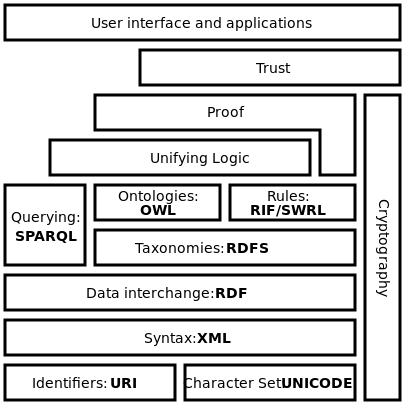
\includegraphics[width=110mm]{Figures/semantic_web_stack.png}
	\caption{The Semantic Web Stack \label{overflow}}
\end{figure}
\begin{itemize}
\item \href{http://en.wikipedia.org/wiki/Resource\_Description\_Framework}{Resource Description Framework}, một phương thức chung để biểu diễn thông tin cho semantic web.
\item \href{http://en.wikipedia.org/wiki/RDF_Schema}{RDF Schema}
\item \href{http://en.wikipedia.org/wiki/Simple_Knowledge_Organization_System}{Simple Knowledge Organization System} (SKOS)
\item \href{http://en.wikipedia.org/wiki/SPARQL}{SPARQL} - Ngôn ngữ truy vấn dữ liệu biểu diễn dưới dạng RDF.
\item \href{http://en.wikipedia.org/wiki/Notation3}{Notation3}, thiết kế với tiêu chí hiểu được bởi con người.
\item \href{http://en.wikipedia.org/wiki/N-Triples}{N-Triples}, một định dạng dùng để lưu và truyền dữ liệu.
\item \href{http://en.wikipedia.org/wiki/Turtle_(syntax)}{Turtle} (Terse RDF Triple Language)
+\item \href{http://en.wikipedia.org/wiki/Web_Ontology_Language}{Web Ontology Language} (OWL), một họ các ngôn ngữ biểu diễn tri thức.

\item \href{}{Rule Interchange Format} (RIF), một framework chung của các ngôn ngữ điều luật web hỗ trợ chuyển đổi nhiều điều luật khác nhau trên web.

\end{itemize}

Hình Semantic Web Stack\cite{semantic3} miêu tả kiến trúc của Semantic Web:

\begin{itemize}
\item XML cung cấp một cú pháp cơ bản nhất cho nội dung bên trong tài liệu, và không có liên quan gì đến mặt ngữ nghĩa mà nội dụng nó chứa. XML không phải là một thành phần cần thiết trong các công nghệ Semantic Web trong hầu hết các trường hợp, tồn tại cú pháp thay thế khác như Turle \textsuperscript{*}. 

\item XML Schema là một ngôn ngữ dùng để cung cấp và hạn chế cấu trúc nội dung của các thành phần nằm trong tài liệu XML, nói cách khác nó giúp chúng ta đáng giá nội dung mà tài liệu đó chứa là gì. Ví dụ: OWL/XML vs. RDF/XML

\item RDF \cite{rdf} là một ngôn ngữ đơn giản dùng để diễn tả các mô hình dữ liệu (ở đây muốn chỉ đến các nguồn dữ liệu web) và mối quan hệ của chúng. Một mô hình dựa theo RDF có thể được biểu diễn bằng nhiều cú pháp khác nhau, vd: RDF/XML, N3, Turtle và RDFa. Có thể nói RDF chính là thành phần cơ bản và quan trọng nhất của Semantic Web.

\item RDF Schema \cite{rdfs} mở rộng RDF và là từ vựng để đặc tả các thuộc tính và lớp trong các tài nguyên dựa trên RDF, với ngữ nghĩa dựa trên các việc tạo ra nhiều phân cấp lớp và thuộc tính.
\item OWL thêm nhiều từ vựng hơn để diễn các thuộc tính và lớp, và điểm quan trọng của nó là thêm các từ vựng để đặc tả mối quan hệ giữa các lớp với nhau. Ví dụ: ranh giới riêng biệt giữa các lớp với nhau (disjointness), các quy định với số lượng (cardinality), cung cấp nhiều loại dữ liệu cho các thuộc tính, và các đặc tính của các thuộc tính (đối xứng/ bất đối xứng, và các lớp liệt kê, ...).

\item SPARQL là một giao thức và ngôn ngữ truy vấn dữ liệu dành cho tài nguyên của Semantic Web.

\item RIF (W3C Rule Interchange Format) là một ngôn ngữ XML để biểu diễn điều luật web mà máy tính có thể thực thi.

\end{itemize}
{\let\thefootnote\relax\footnotetext{*\textit{
			Turtle: http://en.wikipedia.org/wiki/Turtle\_(syntax)}}
}
\paragraph{Kết luận} Trên đây chúng em chỉ liệt kê những thành phần và tiêu chuẩn cơ bản nhất mà tổ chức W3C đã đề ra nhằm xây dựng một mô hình Semantic Web (Web ngữ nghĩa) trong tương lai. Nội dung để tài của chúng em chỉ hạn chế trong việc nghiên cứu và khai thác ngôn ngữ Ontology Web nhằm khai thác tiềm năng về mặc ngữ nghĩa (suy luận ra những thông tin mới dựa trên những suy luận từ ngữ nghĩa của những thông tin được khai báo) nhằm phục vụ cho việc phân loại thông qua các thuộc tính của sản phẩm. Chương kế tiếp sẽ đi qua tìm hiểu về Ontology Web Language(OWL) và Semantic Web Rule Language (SWRL), hai thành phần chính giúp hình thành khả năng phân loại tự động của đề tài này.







%\chapter{Giới thiệu về Semantic Web và Open World Assumption}
Trước khi bắt đầu giới thiệu với sâu hơn về Ontology Web Language (OWL), chúng em xin được giới thiệu qua về giả định Thế Giới Mở (Open World Assumption - OWA) được Semantic Web chấp nhận và phân biệt giả định này với giả định Thế Giới Đóng (Closed World Assumption - CWA).
\begin{description}
\item[Closed World Assumption] 
Giả định Thế Giới Đóng (CWA) là giả định mà những điều không chắc hoặc không có cơ sở để chứng minh là \textbf{đúng} sẽ được chấp nhận là \textbf{sai}.
\item[Open World Assumption]
Giả định Thế Giới Mở (OWA) thì ngược lại, với những điều không chắc hoặc không có cơ sở để chứng minh là \textbf{đúng} sẽ được chấp nhận là \textbf{chưa biết}. 
\item[Ví dụ]
Xem xét một câu nói sau đây: "A là một công dân của nước Mỹ". Nếu có ai đó hỏi "A có phải là một công dân của Việt Nam hay không ?". Xét theo CWA, câu trả lời là \textit{không}, ngược lại với OWA thì câu trả lời là \textit{chưa biết}. 
\end{description}
\section{Vậy OWA và CWA được sử dụng khi nào ?}
Giả định thế giới đóng (CWA) được sử dụng khi một hệ thống đã có đầy đủ thông tin. Đây là trường hợp được áp dụng cho nhiều ứng dụng cơ sở dữ liệu. Ví dụ, xem xét một tình huống một ứng dụng cơ sở dữ liệu đặt vé máy bay, chúng ta tìm kiếm đường bay thẳng Phú Quốc và Hà Nội, và kết quả là nó không tồn tại trong cơ sở dữ liệu (không quan tâm đến thực tế có hay không có đường bay này). Và theo CWA nên câu trả lời từ cơ sở dữ liệu là : "Không có đường bay thẳng Hà Nội - Phú Quốc" (Một giả định là thực tế cũng không tồn tại đường bay này do cơ sở dữ liệu không biết). Đây là dạng ứng dụng mà người dùng mong đợi một câu trả lời chính xác ( phổ biến ở các cở sở dữ liệu quan hệ).
Ngược lại với Giả định thế giới đóng, Giả định thế giới mở đươc áp dụng trên một hệ thống mà thông tin được cung cấp không đầy đủ. Đây là trường hợp chúng ta một biểu dạng một dạng tri thức (a.k.a Ontologies) và chúng ta muốn khám phá những thông tin mới tiềm ẩn trong đó. Ví dụ, xem xét một hệ thống lưu trữ tiền sử bệnh lý của bệnh nhân. Nếu cơ sở dữ liệu không chứa thông tin về một dạng dị ứng cụ thể mà bệnh nhân mắc phải, điều đó không đồng nghĩa là bệnh nhân đó không mắc phải nó trên thực tế. Từ đó câu trả lời từ cở sở dữ liệu theo chuẩn OWA sẽ là : "Không rõ bệnh nhân này có mắc phải dị ứng đó không, trừ khi những thông tin đầy đủ hơn được cung cấp".
\section{CWA vs. OWA: Ví dụ}
Giả định Thế Giới Đóng không chỉ là trả về các câu trả lời \textit{"không"} 

\chapter{Chi tiết Ontology Web Language}
\paragraph{Giới thiệu } - Như đã được đề cập trong phần cuối của chương trước, chức năng chính của OWL là một ngôn ngữ ontology cung cấp ngữ nghĩa cho Semantic Web. Trong nội dung chương này, chúng em sẽ giới thiệu về cú pháp, định dạng và chi tiết các đặc tính của ngôn ngữ Ontology Web. Phiên bản Ontology Web Language chúng em sử dụng là phiên bản 2 được tổ chức W3C khuyến khích sử dụng so với phiên bản OWL 1.1 .
\section{Khái quát về OWL 2 \cite{owl2}}
\subsection{Tổng quan}
\begin{figure}[ht!]
	\centering
	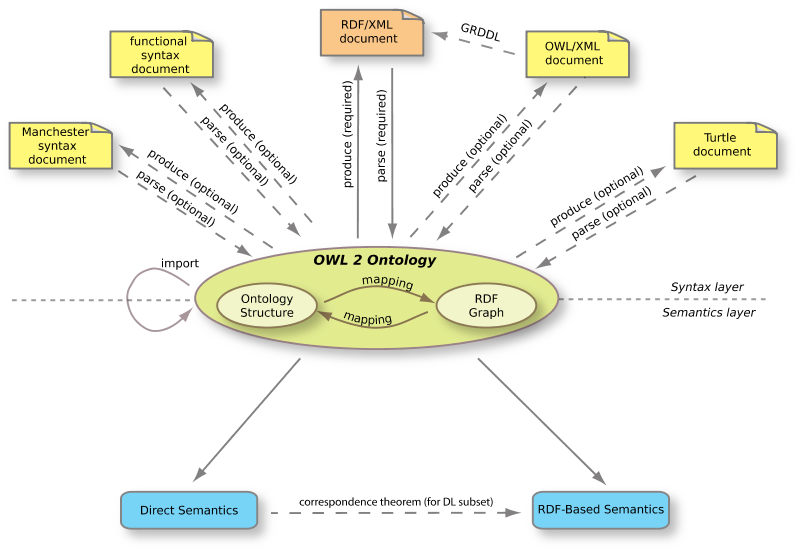
\includegraphics[width=120mm]{Figures/owl2structure.png}
	\caption{Cấu trúc của OWL 2\label{overflow}}
\end{figure}
Hình trên cho chúng ta cái nhìn tổng quan về các định dạng file, các loại cú pháp và cách khả năng serialization thành RDF Graph của Ontology. Như chúng ta thấy trong hình thì hình eclipse ở giữa thể hiện khái niệm trừu tượng của một ontology, có thể hiểu là một cấu trúc trừu tượng hay một đồ thi RDF. Chúng ta có thể dùng nhiều cú pháp để biểu diễn ontology và định dạng chúng dưới dạng file khác nhau (Syntex layer trong hình), các định dạng và cú pháp này hoàn toàn có thể chuyển đổi qua lại với nhau. Lớp ngữ nghĩa trong hình (semantic layer) cho thấy ngữ nghĩa được quy định theo 2 tiêu chuẩn kỹ thuật khác nhau là Direct Semantics và RDF-Based Semantics.
\\
Phần lớn những người phát triển Ontology bằng OWL2 sẽ chỉ cần 1 cú pháp (tương đương với 1 định dạng file) và một dạng biểu diễn ngữ nghĩa.
\subsection{Ontologies}
Bất kì ontology OWL2 nào đều có thể được định dạng như một đồ thị RDF. Mối quan hệ giữa 2 cách này được quy định bới cách tài liệu Mapping to RDF Graphs document [\href{http://www.w3.org/TR/owl2-overview/#ref-owl-2-rdf-mapping}{OWL 2 RDF Mapping}] \cite{mapping_rdf_graph}, trong tài liệu này định nghĩa rất rõ ràng một bảng map từ định dạng cấu trúc của ontology qua đồ thị RDF, và ngược lại. 
\subsection{Cú pháp}
Trong thực tế, một cú pháp cụ thể rất cần thiết để lưu trữ các OWL2 Ontologies và để trao đổi chúng giữa các công cụ và ứng dụng khác nhau. Cú pháp đầu tiên có khả năng hoán đổi là RDF/XML [\href{http://www.w3.org/TR/owl2-overview/#ref-rdf-syntax}{RDF Syntax}] \cite{rdfxml}. Ngoài RDF/XML có khả năng cung cấp khả năng tương tác giữ nhiều ứng dụng OWl2 khác nhau, các loại cú pháp khác đều có thể được sử dụng. Dưới đây là bảng so sánh và liệt kê các cú pháp.
\begin{table}[h]
\begin{tabular}{ |l|l|l|p{4cm}|}

\hline
Tên cú pháp & Mô tả & Trạng thái & Mục đích sử dụng\\
\hline
RDF/XML & Mapping to RDF Graphs \cite{mapping_rdf_graph} \cite{rdfxml} & Bắt buộc & Hoán đổi được ( có thể viết và đọc được bằng nhiều phần mềm OWL2)
\\
\end{tabular}
\caption{Bảng so sánh các cú pháp của OWL2\label{overflow}}
\end{table}
\section{Các đặc tính chi tiết của OWL2}

\chapter{Suy luận với Semantic Web Rule Language}
Nếu chỉ sử dụng các thành phần của  OWL 2 được trình bày ở chương trước thì không thể diễn tả hết tất cả các mối quan hệ trong ontology. Semantic Web Rule Language (SWRL) là một ngôn ngữ điều luật dựa trên nền tảng của OWL. SWRL cho phép người sử dụng khai báo các điều luật dựa trên các khái niệm của OWL như lớp, thuộc tính đối tượng, thuộc tính dữ liệu nhằm cung cấp một khả năng suy luận mạnh mẽ hơn so với chỉ dùng OWL 2. Về đặc tính ngữ nghĩa, SWRL được xây dựng trên cùng một tổ hợp Description Logic với OWL 2 nhưng cung cấp những cơ chế tốt hơn trong việc chỉ ra những thông tin mới đúc kết từ thông tin được khai báo.
%Một ví dụ nổi tiếng là \textit{child of married parent} (con của những cặp ba mẹ là vợ chồng) - sẽ được trình bày ngay sau đây
\section{Cấu trúc của một SWRL Rule}
Một luật SWRL chứa một phần điều kiện, hay còn gọi là rule body, và một phần kết quả, hay còn gọi là rule head. Cả phần body và head đều là giao của các positive atoms.
\begin{center}
$atom$ \verb|^| $atom$ ... -> $atom$ \verb|^| $atom$ 
\end{center}
Có thể hiểu một SWRL Rule theo cách như sau nếu tất cả các thành phần đơn vị (atom) trong phần điều kiện (body) đều đúng (hay xảy ra) thì chắc chắn rằng những ý được nêu ra trong phần kết quả (head) cũng đúng.
\\
Một rule $atom$ được biểu diễn theo dạng:

\begin{center}
$p($ $arg_{1}$, $arg_{2}$, ... $arg_{n}$ $)$
\end{center}

trong đó $p$ là nội dung điều kiện (predicate) và $arg_{i}$, $1<=i<=n$ là những khái niệm hay tham số của mô tả. Trong SWRL, nội dung điều kiện có thể gồm các lớp, thuộc tính hoặc kiêu dữ liệu trong OWL 2. Tham số truyền vào có thể là cá thể, giá trị dữ liệu, hoặc biến để chỉ tới chúng. Tên biến trong cùng một rule không được phép trùng nhau, tên biến của 2 rule khác nhau có thể trùng nhau.

\chapter{Tính nhất quán trong Ontology}
\paragraph{Giới thiệu} Khái niệm tính nhất quán (consistency) đã được nhắc đến nhiều lần trong các chương trước của báo cáo, tính nhất quán ở đây muốn nói đến sự nhất quán về ý nghĩa của những phát biểu trong ontology, tức ý nghĩa của chúng không mâu thuẫn với nhau. Tính nhất quán cực kì quan trọng đối với bất kì một ontology nào, nếu ngữ nghĩa của nội tại của ontology đã không còn sự nhất quán hay tồn tại sự phi lý thì những thông tin được suy luận ra từ ontology cũng trở nên phi lí. Vì vậy quá trình suy luận (reasoning) sẽ không thực hiện được nếu ontology không có tính nhất quán. Trong nội dung chương này, chúng em xin được trình bày các nguyên nhân dễ bắt gặp làm cho ontology không nhất quán trong quá trình phát triển và sử dụng ontology trong các ứng dụng, và chúng em cũng nêu các giải pháp đã được nhiều nghiên cứu thực hiện nhằm tìm ra những lỗi, hay nguy cơ có thể làm cho ontology thiếu nhất quán.
\clearpage
\section{Các nguyên nhân dẫn đến tính thiếu nhất quán trong ontology}
\subsection{Các định nghĩa cần lưu ý \cite{satisfy}}
% Định nghĩa unsatisfiable class
\paragraph{Unsatisfiable Class/Concept} dùng để chỉ một lớp hay một khái niệm trong một ontology mà ngữ nghĩa xung đột với ngữ nghĩa khác được nêu ra trong ontology hay có thể nói là các phát biểu về lớp hay khái niệm này mâu thuẫn với nhau hoặc mâu thuẫn với những phát biểu khác trong ontology.
\begin{description}
	\item[Ví dụ]
	\begin{verbatim}
	Cow
	SubClassOf: Vegetarian
	Vegetarian
	SubClassOf: Animal and eats only Plant
	DisjointClasses:
	Plant, Animal
	\end{verbatim}
	\item[Giải thích]
	Trong ví dụ trên thì MadCow chính là một lớp không hợp lý do trong các phát biểu logic của nó mâu thuẫn với nhau Cow là lớp con của Vegeterian mà Vegeterian chỉ ăn Plant (nghĩa là ngoài Plant, Vegeterian không ăn thứ gi khác) trong khi đó khai báo của lớp MadCow là lớp con của Cow và ăn một số Sheep (Sheep là một lớp con của Animal).
	\\
	Từ đó việc lý luận có thể đưa ra giả định sai là Sheep cũng có khả năng là một phần của Plant . Điểm quan trọng là Plant và Animal là 2 DisjointClasses, nói cách khác không tồn tại một cá thể nào vừa thuộc lớp Plant và vừa thuộc lớp Animal. Như vậy trong tất cả các phát biểu logic ở ví dụ trên đã có 2 phát biểu gây mâu thuẫn chính là eats only Plant và eats some Sheep, và chúng làm cho lớp MadCow trở nên bất hợp lý (unsatisfiable).
\end{description}
% Định nghĩa về incoherent ontology 
\paragraph{Incoherent Ontology} dùng để chỉ một \textit{ontology/model} có ý nghĩa không mạch lạc rõ ràng do nó có chứa ít nhất một \textit{Unsatisfiable Class/Concept} và với điều kiện là trong những \textit{Unsatisfiable Class} này không được chứa bất kì một cá thể (\textit{Individual}) nào.
\\
\hspace{0.05\textwidth} Giả sử ta có ontology A chứa các các phát biếu trong ví dụ trên ngoại trừ phát biểu cuối cùng \texttt{Individual: Dora type: MadCow} thì ta có thể nói ontology A không mạch lạc rõ ràng do nó chứa unsatisfiable class là MadCow. Chúng ta vẫn có sử dụng được ontology A vì nó vẫn còn tính nhất quán (\textit{Consistency})miễn là không có phần tử nào thuộc lớp MadCow.
% Định nghĩa về inconsistent ontology
\paragraph{Inconsistent Ontology} dùng để chỉ một ontology chứa ít nhất một \textit{Unsatisfiable Class} và có ít nhất một cá thể(\textit{Individual}) thuộc một trong những lớp \textit{unsatisfiable} này.
\\
\hspace{0.05\textwidth} Như đã thể hiện trong ví dụ đầu tiên thì cá thể Dora thuộc lớp MadCow (Một lớp unsatisfiable thì không nên phép có bất kì cá thể nào nếu như chúng ta muốn đảm bảo tính consistency cho ontology), như vậy bất kì ontology nào có những phát biểu trên đều được coi là không nhất quán (\textit{inconsistency}), đều này đồng nghĩa là ontology đó không thể sử dụng được nữa.

\subsection{Các nguyên nhân phổ biến dẫn đến tính thiếu nhất quán}
Các nguyên nhân dẫn đến tính thiếu nhất quán trong ontology gây bởi các lỗi được phân loại thành lỗi gây ra bởi phát biểu ở mức độ lớp (Class level - TBox), các lỗi gây ra bởi phát biểu ở mức độ cá thể (Instance/Individual level - ABox)\cite{inconsitentReason} và lỗi gây ra bởi sự kết hợp của cả 2 nguyên nhân vừa nêu trên.
% Instantiating an unsatisfiable class (TBox + ABox)
\subsubsection{Khởi tạo cá thể cho một Unsatisfiable Class) - (TBox + ABox)}
\begin{itemize}
	\item
	Khởi tạo cá thể cho một Unsatisfiable Class được xem là nguyên nhân phổ biến nhất gây ra tính thiếu nhất quán trong ontology.
	\item
	Ví dụ:
	\begin{verbatim}
	Individual: Dora type: MadCow
	\end{verbatim}
	\item
	Chúng ta không quan tâm đâu là nguyên nhân làm cho \texttt{MadCow} trở nên mâu thuẫn, chỉ cần biết là một Unsatisfiable Class thì không nên có bất kì cá thể nào trong đó. Rõ ràng là không có bất kì ontology nào mà cá thể Dora có thể đáp ứng các điều kiện như trong ví dụ đầu tiên, nói cách khác không tồn tại model nào có thể thỏa được điều kiện trên. Chúng ta phát biểu đó là một ontology không nhất quán.
\end{itemize}
% Instantiating disjoint classes (TBox + ABox)
\subsubsection{Khởi tạo cá thể thuộc 2 class được disjoint với nhau (TBox + ABox)}
\begin{itemize}
	\item
	Đây là một trường hợp dễ bắt gặp vì nó sai ngay trong phát biểu về logic.
	\item Ví dụ
	\begin{verbatim}
	Individual: Dora
	Types: Vegetarian, Carnivore
	DisjointClasses: Vegetarian, Carnivore
	\end{verbatim}
	\item
	Lớp A disjoint với B khi và chỉ chi lớp A không có chung bất kì một phần tử/cá thể nào với lớp B. Phát biểu Disjoint Classes(A B C) có nghĩa là mỗi lớp trong đó disjoint với từng lớp còn lại (mutually disjoint). Phát biểu ABox dạng \texttt{DisjointClasses(Vegetarian Carnivore)} là sai vì Dora vừa thuộc Vegetarian vừa thuộc Carnivore dựa vào phát biểu \texttt{Individual: Dora Types: Vegetarian, Carnivore}.
\end{itemize}  	
% Conflicting assertions (ABox)	
\subsubsection{Các phát biểu ABox xung đột với nhau}
\begin{itemize} 
	\item{Trường hợp này thì tương tự như nguyên nhân ở trên nhưng khác ở chỗ là lần này sự mâu thuẫn nằm trong các biểu ở cấp độ cá thể (ABox).}
	\item{Ví dụ:	
		\begin{verbatim}
		Individual: Dora
		Types: Vegetarian, not Vegetarian
		\end{verbatim}
	}
	\item{Dễ thấy được sự mâu thuẫn trong trong phát biểu trên vừa yêu cầu Dora là Vegetarian vừa yêu cầu nó không phải Vegetarian.}
\end{itemize}
% Conflicting axioms with nominals (all TBox)
\subsubsection{Phát biểu xung đột với nghĩa "oneOf" (All TBox)}

\begin{itemize}
	\item 
	Phát biểu bao gồm hoặc một trong (oneOf trong cú pháp của OWL) cho phép sử dụng các cá thể trong khai báo phát biểu ABox, sự kết hợp này có thể dẫn đến sự thiếu nhất quán.
	\item
	Lấy ví dụ sau:
	\begin{verbatim}
	Class: MyFavouriteCow
	EquivalentTo: {Dora}
	Class: AllMyCows
	EquivalentTo: {Dora, Daisy, Patty}
	DisjointClasses: MyFavouriteCow, AllMyCows
	\end{verbatim}
	\item
	Phần đầu tiên của các phát biểu trên tất cả các thể thuộc lớp \texttt{MyFavouriteCow} phải tương đương với cá thể tên Dora, nói cách khác là \texttt{SameIndividual} với \texttt{Dora}. Phần thứ hai cũng  tương tự tất cả các cá thể thuộc lớp \texttt{AllMyCows} buộc phải tương đương với một trong 3 cá thể tên \texttt{Dora}, \texttt{Daisy} hoặc \texttt{Patty}. Do 2 phát biểu trên chúng ta đã nói Dora thuộc cả 2 lớp \texttt{MyFavoriteCow} và \texttt{AllMyCows} nên mâu thuẫn với phát biểu cuối cùng khi nói 2 lớp này không có chung một cá thể nào. Vì vậy dẫn tới ontology bị thiếu nhất quán (inconsistent).
\end{itemize}
% No instantiation possible (all TBox)
\subsubsection{Không có khả năng khởi tạo bất kì cá thể nào (all TBox)}
\begin{itemize}
	\item Ví dụ:
	\begin{verbatim}
	Vegetarian or not Vegetarian
	SubClassOf: Cow and not Cow
	\end{verbatim}
	\item
	Đây chỉ là một ví dụ đơn giản để minh họa cho trường hợp này. Thực tế sẽ ít người dùng nào tạo ra một phát biểu ngớ ngẩn như vậy nhưng nó vẫn có khả năng xảy ra khi phát biểu trên là kết quả từ suy luận (reasoning) của những phát biểu lớn và phức tạp hơn.
	\item
	Có thể giải thích ví dụ trên như sau. Đầu tiên để đáp ứng ý nghĩa dòng đầu tiên yêu cầu cá thể vừa là \texttt{Vegetarian} hoặc không phải \texttt{Vegetarian} - bất kỳ phát biểu nào dạng này, "cá thể thuộc hoặc không thuộc một lớp" chính là tất cả cá thể xuất hiện trong ontology. Dòng thứ hai yêu cầu cá thể vừa là Cow vừa không phải là Cow, phát biểu này rơi vào một trong các nguyên nhân vừa nêu ở trên. Tổng hợp lại chúng yêu cầu tất cả cá thể vừa là Cow vừa không phải Cow, điều này gây ra mâu thuẫn trên toàn ontology do phát biểu đầu tiên chỉ tới tất cả các cá thể.
\end{itemize}

\paragraph{Kết luận}
Trên đây chúng em đã liệt kê những nguyên nhân phổ biến dẫn đến thiếu nhất quán qua những ví dụ đã được đơn giản hoá để dễ dàng nắm bắt được đâu là căn nguyên gây ra sự mâu thuẫn về logic. Trên thực tế với những ontology có số lượng phát biểu lớn và phức tạp rất khó để người dùng có thể nhận diện được đâu là nguyên nhân chính xác gây ra mâu thuẫn, do vậy sự ra đời của một công cụ giúp chúng ta phát hiện chính xác nguyên nhân gây lỗi là rất cần thiết. Vì vậy trong phần tiếp theo, chúng em sẽ đề cập tới debugging một khía cạnh rất được chú trọng đế phát hiện những nguyên nhân gây ra thiếu nhất quán khi số lượng phát biểu của ontology ngày càng tăng.

\section{Giải pháp cảnh báo các nguyên nhân gây ra tính thiếu nhất quán}
{
	\let\thefootnote\relax\footnotetext{
	*\textit{
			Tối ưu có nghĩa là hạn chế tối đa các thay đổi về ý nghĩa mà việc xóa hoặc thay đổi phát biểu mâu thuẫn có thể gây ra cho các phát biểu khác (other axioms) trong ontology.
	}}		
	\let\thefootnote\relax\footnotetext{
		**\textit{
			Mọi quan điểm và ý tưởng trình bày ở phần sau của mục này đều thuộc của các tác giả bài báo \cite{repair} và \cite{matt_horridge}. Chúng em chỉ trình bày lại sau khi đã đọc và nắm được ý tưởng chính yếu của bài báo.
	}}
}
\begin{itemize}
\item Như đã được đề cập trong phần trước, trong các nguyên nhân dẫn đến tính thiếu nhất quán (\textit{inconsistency}) trong ontology thì \textbf{unsatisfiable Class} (lớp không thỏa về tính logic) là nguyên nhân nếu có thể được phát hiện sớm để loại bỏ hoặc sửa lại các phát biểu gây mâu thuẫn thì giúp cho ontology tránh bị inconsistent.
\item Đã có rất nhiều nghiên cứu thành công trong việc tìm và phát hiện lỗi (các phát biểu mâu thuẫn) trong ontology. Trong đó có một nghiên cứu nổi bật\cite{repair}, không chỉ có khả năng phát hiện gần như chính xác các nguyên nhân gây lỗi mà còn được đưa ra các giải pháp tối ưu\textsuperscript{*} để sửa lỗi. Nghiên cứu này đã được ứng dụng để đưa ra các giải thích về các lớp không thỏa về nghĩa (unsatisfiable classes) trong bộ thự viện lập trình ontology thông dụng hiện nay là OWL-API\cite{owlapi}. Sau đây chúng em xin được trình bày lại những điểm quan trọng trong nghiên cứu vừa được đề cập\textsuperscript{**}
\end{itemize}

		
\subsection{Mục tiêu của việc debuging ontology}
Mục tiêu chính của việc debuging ontology gồm hai phần quan trọng. Thứ nhất, với một ontology có số lượng lớn các lớp unsatisfiable, cần tìm và nhận dạng được nguyên nhân gây ra mâu thuẫn và các lớp bị ảnh hưởng bởi sự mâu thuẫn đó trong ontology. Thứ hai, cho biết trước một Unsatisfiable Class cụ thể, trích xuất và trình bày cho người sử dụng ontology(\textit{modeler}) một tập hợp tối tiểu các phát biểu (\textit{minimal set of axioms}) từ ontology hay nguyên nhân chính xác chịu trách nghiệm trong việc gây ra sự mâu thuẫn về logic.
\\
\subsection{Khái niệm và các kỹ thuật cần biết}
Các hệ thống Description Logic thường cung cấp một tập hợp các tác vụ suy luận đã được chuẩn hóa như phân loại các khái niệm (\textit{concept classification}), kiểm tra tính đáp ứng về logic (\textit{concept satisfiability}) và kiếm tra tính nhất quán của knowledge base (KB). Hầu hết các reasoner thông dụng hiện nay đều buộc phải cung cấp đủ 3 tác vụ nêu trên, nhưng tất cả chúng đều không thân thiện với người dùng. Do tất cả những gì chúng ta biết được đều là kết quả (hay output) từ sự suy luận(reasoning) của reasoner. 
\\
\hspace*{0.05\textwidth}  Để giúp cho các tác vụ suy luận (reasoning) trở nên thân thiện với người dùng hơn, một hệ thống DL-based Knowledge Representation (KR) phải mở rộng thêm các lựa chọn về các tác vụ không nằm trong tiêu chuẩn của DL. Một ví dụ cụ thể là việc tạo ra các giải thích tại sao một lớp lại bị reasoner đánh giá là unsatisfiable. Thêm một tình huống mà người dùng cần được giải thích là tại sao reasoner đánh giá một lớp là lớp con của một lớp khác - đâu là lý do. Việc ra đời tác vụ giải thích nguyên nhân và kết quả là thật sự cần thiết trong bối cảnh sự phát triển nhanh của Semantic Web và cộng đồng người dùng/nhà phát triển Ontology ngày càng tăng nhanh.
\subsubsection{Dịch vụ Axiom Pinpointing}
\paragraph{Axiom Pinpointing service} chính là dịch vụ có khả năng thực hiện tác vụ giải thích vừa được đề cập, với một KB và bất kì kết quả suy luận nào từ KB, dịch vụ này sẽ trả về tập các chứng minh/giải thích cho suy luận đó bằng những phát biểu đã được khai báo trong KB.
\\
\hspace*{0.05\textwidth} Có thể giải thích ngắn gọn như sau \cite[p.~2]{axiomPinpoint}, cho một phát biểu kết quả họ SHOIN $\alpha$ được suy ra từ một knowledge base $K$, một kiểm chứng (justification) cho $\alpha$  trong $K$ là một phần tối tiểu $K^{'}\subseteq$ $K$ chịu trách nhiệm cho $\alpha$ xảy ra. Kiểm chứng $K^{'}$ là tối tiểu với điều kiện $\alpha$ là một kết quả logic được suy ra từ $K^{'}$, hay nói cách khác $K^{'}$ tối tiểu khi và chỉ khi bất kì tập con nào của $K^{'}$ đều không suy ra được $\alpha$. Nói chung có thể tồn tại nhiều giải thích/chứng minh cho $\alpha$ trong $K$. Sau đây là một ví dụ cho ý tưởng vừa nêu. Cho KB $K$ với các phát biểu như sau:
\begin{enumerate}
	\item	$A$ $\subseteq$ $B$ $\cap$ $C$ 
	\item	$B$ $\subseteq$ $\neg$ $E$
	\item	$A$ $\subseteq$ $D$ $\cap$ $\exists$ $R.E$ 
	\item	$D$ $\subseteq$ $C$ $\cap$ $\forall$ $R.B$
\end{enumerate}
		
Trong KB trên, $A, B, C, D, E$ là atomic concepts và $R$ là atomic role.  Chúng ta sẽ dùng số thứ tự của từng câu phát biểu trên thay vì lặp lại nguyên văn.
 
\hspace*{0.05\textwidth} Từ các phát biểu trên ta có $K$ $\models$ ($A$ $\subseteq$ $C$). Tuy nhiên, điều kiện cần và đủ để suy ra được một kết quả tương tự từ 2 phần nhỏ hơn của KB $K$ là $K_{1}$ = {1} và $K_{2}$ ={3,4}. Chúng ta nói $K_{1}$ và $K_{2}$ là các kiểm chứng cho kết luận nói $C$ là tập con của $A$ - $A$ $\subseteq$ $C$.

\hspace*{0.05\textwidth} KB trong ví dụ vừa nêu được xem là khá nhỏ, qua đó dễ dàng nhận ra lợi ích đáng kể khi số lượng phát biểu trong KB tăng lên vài trăm hay vài ngàn phát biểu. Bằng cách nhận dạng chính xác các tập tối tiểu chứa các phát biểu khẳng định (asserted) là những giả thiết cho kết quả được suy ra, dịch vụ này có thể được dùng để cô lập, đánh dấu và giải thích nguyên nhân hoặc cơ sở của các kết quả suy luận. Điều này cực kì quang trọng trên khía cạnh debugging, lấy ví dụ trường hợp cần giải thích là một Unsatisfiable Class/Concept, dịch vụ này sẽ khám phá tất cả và chỉ những phát biểu là nguyên nhân gây lỗi. Trong trường hợp vừa nêu, tìm kiếm tất cả các kiểm chứng là rất cần thiết vì để sửa lại unsatisfiable class cần loại bỏ ít nhất một phát biểu trong tập các phát biểu tối tiểu nguyên nhân gây lỗi MUPS - sẽ được đề cập trong mục bên dưới.

\hspace*{0.05\textwidth} Tuy nhiên, dịch vụ axiom pinpointing chúng ta đề cập có một giới hạn là nó chỉ làm việc ở mức độ giữa các phát biểu với nhau, chúng vẫn chưa phân biệt được phần cụ thể nào của phát biểu mới là nguyên nhân cần và đủ để giải thích cho kết quả suy luận. Lấy lại ví dụ vừa nếu trên KB $K$, lớp $B$ trong giao của $B$ $\cap$ $C$ trong phát biểu 1, không phải là giải thiết cần để suy ra $A$ $\subseteq$ $C$. Tương tự, $\exists$ $R.E$ và $\forall$ $R.B$ trong phát biểu 3 và 4 không phải điều kiện cần để suy ra được $A$ $\subseteq$ $C$. 

\hspace{0.05\textwidth} Do vậy, việc quan tâm xem phần nào của phát biểu mới chính là giả thiết/nguyên nhân của kết quả suy luận rất quan trọng trong nhiều trường hợp, đặc biệt khi sửa chữa một phát biểu gây lỗi thì việc sửa lại một phần của phát biểu sẽ hạn chế sự mất mát về ý nghĩa của ontology hơn là xóa nó đi.

\hspace*{0.05\textwidth} Để đáp ứng yêu cầu này, họ để định nghĩa một \textit{hàm chia nhỏ KB}. Ý tưởng là viết lại một phát biểu bất kì trong KB thành những dạng tập gồm các phát biểu nhỏ và đơn giản hơn với ý nghĩa  tương đương. Sau đó, sử dụng \textit{Axiom Pinpointing Service} lên những tập những phát biểu trong KB $K_{s}$ đã được viết lại từ $K$ để tìm kiếm nguyên nhân hay giải thích cho kết quả suy luận. Lấy phát biểu 1 trong ví dụ trên:
\begin{center}
	$A$ $\subseteq$ $B$ $\cap$ $C$ (1) được viết lại thành $A$ $\subseteq$ $B$, $A$ $\subseteq$ $C$ (1\textsuperscript{*})
\end{center}
Dễ dàng thấy phần $A$ $\subseteq$ $C$ trong 1\textsuperscript{*} chính là điều phải chứng minh cho $K$ $\models$ ($A$ $\subseteq$ $C$), những phần còn lại không cần thiết. Tương tự, ta viết lại (3) và (4) như sau:
\begin{center}
	$A$ $\subseteq$ $D$ $\cap$ $\exists$ $R.E$  $\Leftrightarrow$ $A$ $\subseteq$ $D$, $A$ $\subseteq$ $\exists$ $R.E$
	\\
	$D$ $\subseteq$ $C$ $\cap$ $\forall$ $R.B$ $\Leftrightarrow$ $D$ $\subseteq$ $C$, $D$ $\subseteq$ $\exists$ $R.B$
\end{center}
Bây giờ, điều kiện cần và đủ để chứng minh $K$ $\models$ ($A$ $\subseteq$ $C$) là $A$ $\subseteq$ $D$ và $D$ $\subseteq$ $C$. Tuy nhiên, trong một vài trường hợp "hàm chia nhỏ KB" này đòi hỏi phải giới thiệu ra một tên lớp mới, viết giới thiệu tên lớp mới này chỉ phục vụ cho mục đích viết lại phát biểu. Ví dụ:	
\begin{center}
	$A$ $\subseteq$ $\exists$ $R.$ ($C\cap$ $D$) không tương đương với $A$ $\subseteq$ $\exists$ $R.C$, $A\subseteq$ $\exists$ $R.D$
\end{center}
Để chia nhỏ phát biểu trên chúng ta sẽ giới thiệu một tên lớp mới, gọi là $E$.	Như vậy ta có:
\begin{center}
	$A$ $\subseteq$ $\exists$ $R.$ ($C$ $\cap$ $D$) $\Leftrightarrow$ $A\subseteq$ $\exists$ $R.E$, $E\subseteq$ $C$, $E\subseteq$ $D$, $C\cap$ $D\subseteq$ $E$
\end{center}
Để thực hiện được cái gọi là \textit{"hàm chia nhỏ KB"} các bài báo \cite{repair} và \cite{axiomPinpoint} đã đề xuất các giải thuật với tiêu chí xác định các phát biểu chứng minh một cách đầy đủ và chính xác. Các giải thuật này có thể được chia thành 2 nhóm:
\begin{enumerate}
	\item \textit{Reasoner Dependent(or Glass-box) Algorithm} Đây là nhóm các giải thuật xây dựng trên quy trình đưa ra quyết định Tableau dành cho Description Logic. Tuy nhiên, để áp dụng các giải thuật loại này trong thực tế đòi hỏi phải có những chỉnh sửa đáng kể bên trong quy trình suy luận những DL reasoner hiện nay.
	\item \textit{Reasoner Independent(or Black-box) Algorithm} Nhóm này chỉ sử dụng các DL reasoner cho những tác vụ kiểm tra lại kết quả suy luận khi đã viết lại KB $K$ thành $K^{'}$, chúng không đòi hỏi phải chỉnh sửa lại các cách hoạt động của reasoner. Reasoner lúc này có chức năng như một "chiếc hộp đen" chấp nhận các input là lớp/các phát biểu đã được viết lại hoặc một KB $K^{'}$ viết lại từ KB $K$, sau đó trả về output là một câu trả lời xác nhận hay phủ định rằng các lớp và các phát biểu này có là tập tối tiểu để chứng minh cho kết quả suy luận hay không. Ví dụ trong trường hợp:
	\begin{center}
		$A$ $\subseteq$ $B$ $\cap$ $C$ $\Leftrightarrow$ $A$ $\subseteq$ $B$, $A$ $\subseteq$ $C$
	\end{center}
	Các inputs của reasoner sẽ lần lượt sau mỗi vòng là 
	\begin{enumerate}
		\item $A$ $\subseteq$ $B$, $A$ $\subseteq$ $C$
		\item $A$ $\subseteq$ $B$
		\item $A$ $\subseteq$ $C$
	\end{enumerate}
	Giải thuật sẽ lần lượt loại bỏ từng phát biểu một (sau mỗi vòng) để xem những phát biểu còn lại có đủ chứng minh  $K$ $\models$ ($A$ $\subseteq$ $C$). Đến khi nào giải thuật không tồn tại tập phát biểu nào đủ để chứng minh $K$ $\models$ ($A$ $\subseteq$ $C$) thì sẽ dừng vòng lặp.
\end{enumerate}
Kết luận: trên đây chỉ là những bước hoạt động cơ bản nhất của Axiom Pinpointing Service và Blackbox Algorithm xin đọc thêm \cite{axiomPinpoint}. Các giải thuật và dịch vụ này cũng đã được áp dụng trong package  com.clarkparsia.owlapi.explanation của \cite{owowlapi} sẽ được giới thiệu ở chương sau.
\subsubsection{Minimal Unsatisfiability Preserving Sub-TBoxes (MUPS)}
Khái niệm MUPS lần đầu được giới thiệu trong\cite{mups}.Như đã được để cập trong phần đầu của mục này, một MUPS thật ra chính là một phần nhỏ nhất của KB $K$ mà trong đó lý giải tại sao một lớp lại unsatisfiable, nói cách khác một MUPS là một tập tối tiểu các phát biểu mà trong đó các phát biểu này giải thích chính xác nguyên nhân gây ra mâu thuẫn về logic(unsatisfiable). Một lớp unsatisfiable có thể có nhiều MUPS trong KB $K$ (hay cụ thể là trong ontologies). Ví dụ có KB $K_{\alpha}$ với những phát biểu như sau:
	\begin{enumerate}
		\item $S$ $\equiv$ $A$ $\cap$ $\exists$ $R.B$
		\item $S$ $\subseteq$ $\exists$ $R$.($C$ $\cap$ $D$) 
		\item ($C$ $\cap$ $D$) = $\emptyset$ 
	\end{enumerate}
	Dựa vào các phát biểu trên ta thấy $S$ unsatisfiable. MUPS của $S$ từ $K_{\alpha}$ là:
	\begin{center}
		$S$ $\subseteq$ $\exists$ $R$.($C$ $\cap$ $D$) (2)
		\\
		($C$ $\cap$ $D$) = $\emptyset$ (3)
	\end{center}
Để sửa lại một lớp không đáp ứng(\textit{unsatisfiable class}) chúng ta cần loại bỏ tối thiểu ít nhất một phát biểu từ từng tập các phát biểu tối tiểu MUPS lý giải cho unsatisfiable class đó. Trong ví dụ vừa rồi do chỉ có 1 MUPS, ta bỏ tất cả các phát biểu trong MUPS xuất hiện trong KB $K_{\alpha}$ thì $S$ sẽ lại \textit{satisfiable}.
\subsection{Các bước sửa chữa các phát biểu bị lỗi}
\subsubsection{Tìm tất cả các MUPS của một Unsatisfiable Class}
Như vừa nói ở trên MUPS thật ra chính là một phần nhỏ nhất trong KB khiến cho một lớp unsatisfiable. Do vậy tìm và xác định MUPS chính là tìm và xác định các tập tối tiểu các phát biểu cho một lớp được suy luận là  unsatisfiable. Chúng ta sẽ sử dụng \textit{Axiom Pinpointing Service}\cite{axiomPinpoint} để tìm MUPS với các bước tương tự đã được mô tả chi tiết trong mục trên. Nhiệm vụ tìm kiếm \textit{precise} MUPS của lớp không đáp ứng trong KB \textit{K} được đơn giản hóa thành vấn đề tìm MUPS trong những phiên bản đã được tách nhỏ trong KB $K_{s}$.
\subsubsection{Chiến thuật xếp hạng các phát biểu (\textit{Axioms})}
Đây là một giai đoạn khá quan trọng trong quá trình chỉnh sửa lại các phát biểu gây lỗi, quyết định xem nên loại bỏ phát biểu nào từ các MUPS để lớp/khái niệm được satisfiable.

\hspace*{.05\textwidth} Với mục tiêu này, một nhân tố đáng quan tâm là các phát biểu trong MUPS có thể được \textit{xếp hạng} dựa theo mức độ quan trọng của chúng. Việc sửa chữa các nguyên nhân gây lỗi được trở thành một vấn đề cần được tối ưu để đáp ứng các tiêu chí vừa phải loại bỏ tất cả các lỗi gây ra tính thiếu nhất quán trong ontology, trong khi vẫn chắc chắn rằng những phát biểu có thứ hạng cao, nói cách khác là có giá trị quan trọng về nghĩa sẽ được ưu tiên giữ lại và các phát biểu có thứ hạng thấp nhất sẽ bị loại bỏ.

\hspace*{.05\textwidth} Tiêu chí đơn giản nhất để xếp hạng các phát biểu là đếm số lần chúng xuất hiện trong MUPS từ những lớp unsatisfiable xuất hiện trong một ontology. Nếu một phát biểu xuất hiện trong $n$ MUPS khác nhau (trong từng tập phát biểu của MUPS), bỏ đi phát biểu đó sẽ đảm bảo rằng $n$ lớp/khái niệm được satisfiable. Số lần phát biểu xuất hiện càng nhiều, thứ hạng của nó càng thấp.

\hspace*{0.05\textwidth} Ngoài tần suất xuất hiện của phát biểu  trong MUPS, chúng ta cũng có thể quan tâm đến những yếu tố sau để đưa vào tiêu chí xếp hạng:
\begin{itemize}
	\item Tác động lên ontology khi loại bỏ phát biểu hoặc thay đổi nội dung phát biểu - cần phải nhận diện được những tác động tối tiểu (\textit{minimal impact})  gây ra thay đổi.
	\item Tự xây dựng những test cases cụ thể để xếp hạng các phát biểu dựa theo tiêu chí của người dùng tự đề ra.
	\item Dựa trên những metadata của phát biểu như tác giả, độ tin cậy của nguồn tài liệu, timestamp, etc.
	\item Sự liên quan tới ontology ở khía cạnh phát biểu được sử dùng vào mục đích gì và sử dụng như thế nào.
\end{itemize}
Lưu ý: Chi tiết về cách áp dụng từng tiêu chí xếp hạng trên xin đọc \cite{repair}.
\subsubsection{Tạo ra các giải pháp sửa lỗi}
	Qua các phần trên, chúng ta đã biết được làm thế nào để tìm MUPS cho một lớp unsatisfiable bằng Axiom Pinpointing Service trong một OWL-DL ontology và thấy được một loạt các tiêu chí để xếp hạng phát biểu trong MUPS. Bước tiếp theo là tạo ra một kế hoạch sửa lỗi (hay một loạt các thay đổi trong ontology) để sửa các lỗi trong một tập các lớp/khái niệm bị unsatisfiable, với các dữ kiện đã có qua các bước trên như các MUPS tìm được và thứ hạng các phát biểu để chính sửa.
	
	\paragraph{Điều chỉnh giải thuật Reiter} Giải thuật Hitting Set của Reiter\cite{hst}, đưa ra nhằm để xác định căn nguyên(\textit{root cause}) của một vấn đề từ một bộ(\textit{collection}) gồm nhiều tập hợp đụng độ chứa các nguyên nhân dẫn tới vấn đề, giải thuật này sẽ tạo ra những tập tối tiểu (\textit{minimal hitting set}) chứa các nguyên nhân gây ra vấn đề. Một tập hợp đụng độ (\textit{hitting set}) trong một bộ \textbf{C} các tập hợp là tập hợp giao (có chung phần tử) với từng tập hợp trong \textbf{C}. Một tập hợp đụng độ là tối tiểu nếu không có bất kì tập con nào của nó lại là một tập đụng độ cho \textbf{C}. Trong trường hợp của chúng ta, bộ \textbf{C} chứa các HST chính là các MUPS tìm được trong ontology.  \\\hspace*{.05\textwidth} Ý tưởng là áp dụng giải thuật Reiter để tìm ra tập tối tiểu các phát biểu gây lỗi từ các MUPS đã tìm được, rồi loại bỏ tất cả các phát biểu trong tập đụng độ tối tiểu từ đó giúp loại bỏ từng phát biểu gây lỗi xuất hiện trong từng tập phát biểu từng MUPS và cuối cùng giúp cho sửa chữa được cho lớp/khái niệm được satisfiable. Nguyên lý tương tự cũng được áp dụng cho việc giải pháp sửa lỗi ngoại trừ cần phải điều chỉnh lại giải thuật HS để nó có thể hoạt động dựa trên thứ hạng của các phát biểu.
	
	\hspace*{.05\textwidth} Cho một bộ $C$ gồm những tập đụng độ, giải thuật Reiter giới thiệu một khái niệm về hitting set tree (HST), là một cấu trúc cây có số cạnh nhỏ nhất và số node nhỏ nhất, với cạnh và node đều được dán nhãn (labeled). Một node $n$ trong HST được dán nhãn bởi dấu tick (\cmark) nếu $C$ rỗng, ngược lại node này sẽ được dán nhãn bởi bất kì tập hợp $s$ $\in$ $C$. Với mỗi node $n$, ta có $H(n)$ là tập gồm các nhãn của cạnh (edge labels) trên đường đi từ gốc cây tới $n$ (root to $n$); và nhãn cho $n$ là bất kì tập $s$ $\in$ $C$, thỏa điều kiện $s$ $\cap$ $H(n)$ $\Leftarrow$ $\emptyset$, nếu có một tập hợp nào như vậy tồn tại. Nếu $n$ được dán nhãn bởi một tập $s$, thì với từng $\sigma$ $\in$ $s$, $n$ có một node kế cận là $n_{\sigma}$ nối với $n$ bởi một cạnh được dán nhãn bằng $\sigma$. Với bất kì node nào được dán nhãn bằng \cmark , tập chứa các nhãn mô tả đường đi (theo cạnh) của node này tới gốc cây là một tập đụng độ(hitting set) của $C$. Khi tạo ra HST từ gốc, nếu trong quá trình tìm kiếm phát hiện được giải một giải pháp tối ưu hiện thời, thì quá trình sẽ được kết thúc sớm hơn, đánh dấu bằng một bằng dấu chéo (\xmark) trên nhãn của node.
	
	\hspace*{.05\textwidth} Áp dụng vào trường hợp của chúng ta, MUPS của các lớp unsatisfiable tương đương với các tập hợp đụng độ. Tuy nhiên, trong giải thuật HST bình thường được tối ưu theo tiêu chí đường đi ngắn nhất, thay vì đường đi ngắn nhất chúng ta sẽ sử dụng thứ hạng nhỏ nhất (minimal path rank), nói cách khác tổng thứ hạng của các phát biểu trong $H(n)$ sẽ phải nhỏ nhất. Thêm nữa, là trong giải thuật HST cơ bản, không tồn tại khái niệm lựa chọn một phát biểu trong những phát biểu khác trong khi xây dựng cạnh của HST, trong khi chúng ta có thể sử dụng thứ hạng của các phát biểu trong lúc quyết định lựa chọn để thu hẹp không gian tìm kiếm, hay nói dễ hiểu là trong mỗi giai đoạn xây cạnh chúng ta sẽ chọn phát biểu có thứ hạng thấp nhất.
	
	\hspace*{.05\textwidth} Hình 2.1 Thể hiện một HST của một collection $C$ chứ các phát biểu từ 1 - 7  $C$ = {{2,5}, {3,4,7}, {1,6}, {4, 5, 7}, {1, 2, 3}} với thứ hạng của các phát biểu từ 1 - 7 như sau: $r(1) = 0.1, r(2) = 0.2, r(3) = 0.3, r(4) = 0.4, r(5) = 0.3, r(6) = 0.3, r(7) = 0.5$, trong đó $r(x)$ là hạng của phát biểu $x$. Thứ hạng này được tính ra dựa trên những yếu tố được đề cập ở phần 2.3.2 như tần suất xuất hiện, tác động ngữ nghĩa, etc. mỗi tiêu chí được đánh gía riêng biệt, nếu cần chúng ta có thể quy ước một hệ số để đánh giá tất cả cùng một lúc. Số mũ trên từng phát biểu chính biểu diễn hạng của phát biểu đó, và $P_{r}$ là \textit{path rank} được tính bằng tổng hạng của các phát biểu nằm trên đường đi (theo cạnh) từ gốc tới một node. Ví dụ, cạnh cận trái nhất có \textit{path rank}: $P_{r}$ = 0.2 + 0.3 + 0.1 + 0.3 = 0.9.
	\begin{figure}[ht!]
			\centering
			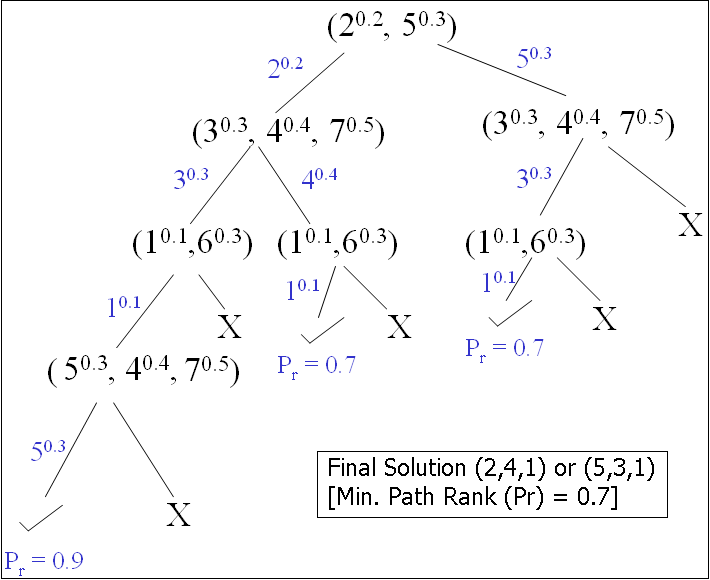
\includegraphics[width=90mm]{Figures/fig1.png}
			\caption{Giải thuật HST được chỉnh sửa dựa theo thứ hạng của phát biểu \label{overflow}}
	\end{figure}
	
	\hspace*{.05\textwidth} Như được thể hiện trong hình, bằng cách chọn phát biểu có hạng thấp nhất trong từng tập trong khi xây cạnh của HST, giải thuật chỉ tạo ra 3 hitting sets, 2 trong số đó tối tiểu, trong khi hạn chế được một số lượng lớn số lần kiểm tra đường đi, (thể hiện bằng \xmark). Giải pháp sửa lỗi được tìm ra trong tập có $P_{r}$ nhỏ nhất là {2,4,1} hoặc {5,3,1}.
	
	\hspace*{.05\textwidth} Tuy vậy, có một hạn chế khi sử dụng quy trình vừa nêu trên để tạo ra kế hoạch sửa lỗi, như phân tích tác động ngữ nghĩa của phát biểu chỉ được thực hiện ở cấp độ là một phát biểu đơn lẻ, trong khi một loạt tác động khác chưa được tính tới mỗi lần một HS được tìm thấy. Điều này có thể dẫn tới một giải pháp kém tối ưu. Ví dụ:
	\begin{enumerate}
		\item	DisjointClasses(Car Plane Ship)
		\item	EquivalentClass(FlyingCar (Car and Plane))			
	\end{enumerate}
	Trong ví dụ trên, bỏ \texttt{Plane} ra khỏi phát biểu (1) sẽ hạn chế mất mát về nghĩa hơn là xóa hết cả phát biểu (1), vì có thể disjoint giữa Car và Ship có thể được sử dụng đâu đó trong ontology mà chưa được tính đến.
	\hspace*{.05\textwidth} Để khắc phục hạn chế này, một chỉnh sửa khác được đưa ra là cứ mỗi lần tìm ra hitting-set(HS), chúng ta sẽ tính lại thứ hạng của đường đi (path-rank) cho HS dựa trên một loạt tác động của các phát biểu trong hitting-set. Giải thuật bây giờ sẽ tìm được giải pháp tối thiểu được path-ranks mới.
	\\
	Trên đây là ý tưởng cơ bản của giải thuật HST, ngoài ta còn những mục về cải thiện các giải pháp sửa lỗi và gợi ý các phát biểu sửa lỗi xin đọc thêm ở \cite{repair}.
	
\subsection{Ứng dụng HST để xác định tất cả giải thích cho kết quả suy luận\cite{matt_horridge}}
Ngoài ứng dụng vừa được đề cập ở trên, Hitting Set Tree còn được áp dụng để tìm tất cả các giải thích cho một kết quả suy luận, giống như một trong chức năng chính của Axiom Pinpointing Service được đề cập lúc nãy. Tuy nhiên, không giống như khái niệm HST của Reiter vừa được giới thiệu ở trên, ở đây chúng ta sẽ có HST với quy ước như sau.

\hspace*{.05\textwidth} Với ontology $\beta$ $\models$ $\eta$, một cây hitting set (HST) cho $\eta$ trong $\beta$ là một cây hữu hạn, bao gồm node được dán nhãn bằng các kiểm chứng(justifications) hay các phát biểu chứng minh $\beta$ $\models$ $\eta$ và cạnh được đánh dấu với phát biểu trong $\beta$. Từng non-leaf(không phải lá) node $v$ nối với một node kế cận $v^{'}$ qua một cạnh được dán nhãn với một phát biểu $\alpha$ với $\alpha$ nẳm trong nhãn của $v$, nhưng không nằm trong nhãn của $v^{'}$. Nhãn của $v^{'}$ có thể là một tập hợp rỗng, trong trường hợp đó $v^{'}$ phải là node lá (leaf node). Ngoài ra, với bất kì node $v^{''}$, tập chứa các phát biểu dán nhãn cho đường đi từ $v^{''}$ tới gốc cây (tree root) \textit{không} giao với kiếm chứng(hay các phát biểu chứng minh) dán nhãn $v^{''}$.

\hspace*{.05\textwidth} Quá trình xây dựng HST có thể được thực hiện bằng các giải thuật \textit{breadth first} hay \textit{depth first}. Dù được sử dụng theo cách nào, các nguyên lý và các luật để tạo và dán nhãn cạnh, node trên cây đều như nhau. Khi mở rộng cây từ node $v$ đến một node mới $v^{'}$ quy trình cơ bản đều diễn ra như sau:
		\begin{enumerate}
			\item Chọn một phát biểu $\alpha$ nẳm trong nhãn của $v$ nhưng không dán nhãn một cạnh nối $v$ tới bất kì node kế cận nào.
			\item Gọi $S$ là hội của (union of) {$\alpha$} và tập những phát biểu nằm trên cạnh, tạo thành đường đi từ $v$ tới root node. Loại bỏ $S$ khỏi $\beta$ ta được $\beta^{'}$.
			\item Nếu $\eta$ thỏa $\beta^{'}$ $\models$ $\eta$ thì tìm một kiểm chứng (justification) $J$ cho $\eta$ trong $\beta^{'}$. Nếu $\beta^{'}$ $\not\models$ $\eta$ thì gán $J$ = $\emptyset$.
			\item Tạo một node mới $v^{'}$ và dán nhãn cho $v^{'}$ bằng tập $J$ ở bước trên.
			\item Tiếp tục mở rộng HST theo một hướng bằng cạnh $e$ = ($v$, $v^{'}$) tương tự như bước 1 cho tới khi không tìm được tập $J$ = $\emptyset$ như ở bước 2.
			\item Đưa các phát biểu trong $S$ trở lại $\beta$.
		\end{enumerate}
		Ví dụ sau mô tả lại quy trình trên, cho ontology $\beta$  với các phát biểu sau:
		\begin{enumerate}
			\item $A$ $\subseteq$ $B$
			\item $B$ $\subseteq$ $D$ 
			\item $A$ $\subseteq$ $\exists$ $R.C$ 
			\item $\exists$ $R.\top$ $\subseteq$ $D$
		\end{enumerate} 

Trong đó $\eta$ $=$ $A\subseteq$ $D$. HST cho $\beta$ $\models$ $A$ $subseteq$ $D$ được thể hiện ở hình 2.2. Bắt đầu di chuyển tại root node, node được dán nhãn bởi $J_{1}$\textsuperscript{*}, mở rộng HST về phía bên trái bằng cách chọn phát biểu $A\subseteq$ $B$ trong $J_{1}$ với điều kiện $A\subseteq$ $B$ chưa dán nhãn bất kì cạnh nào nối với root node sau đó loại bỏ phát biểu $A\subseteq$ $B$ khỏi $\beta$ và tính toán lại kiếm chứng (justifications) thỏa $\langle\beta$ $\backslash$ $\{A\subseteq$ $B\}\rangle$ $\models$ $A\subseteq$ $D$. Trong trường hợp này, chúng ta tìm được kiểm chứng $J_{2}$ trong $\beta$ $\backslash$ $\{A\subseteq$ $B\}$, giải thích được tại sao $A\subseteq$ $D$. Tiếp tục đi về phía bên trái của node $J_{2}$, chọn $A\subseteq$ $\exists$ $R.C$ trong $J_{2}$ tương tự cách chọn ở bước 1. Sau đó tìm kiếm các kiểm chứng trong $\beta^{'}$ $\equiv$ $\beta$ $\backslash$ $\{A\subseteq$ $\exists$ $R.C$, $A\subseteq$ $B\}$, kết quả là chúng ta không tìm được kiểm chứng trong $\beta^{'}$ giải thích cho $A\subseteq$ $D$ hay có thể nói là $\beta^{'}$ $\not\models$ ($A\subseteq$ $D$), do vậy node kế được dán nhãn bằng $\emptyset$ vì lúc này $J$ $=$ $\emptyset$ (bước 3). Mỗi lần như vậy ta tìm ra leaf-node, chúng ta sẽ đưa $S$ trở lại $\beta$ và bắt đầu lại quá trình tìm kiếm.
		\begin{figure}[ht!]
			\centering
			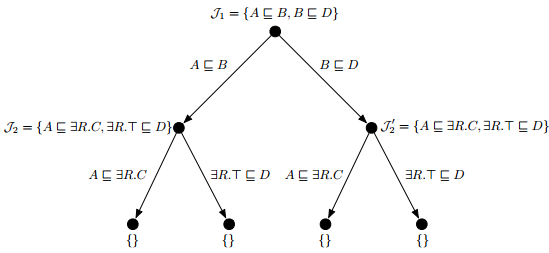
\includegraphics[width=110mm]{Figures/fig2.png}
			\caption{Hitting Set Tree dùng để tìm kiếm kiểm chứng \label{overflow}}
		\end{figure}
% A foot note
{\let\thefootnote\relax\footnotetext{*\textit{
					$J_{1}$,$J_{2}$,$J_{2}^{'}$ được tính ra nhờ giải thuật Black-box hoặc Glass-box được đề cập ở trên.
}}
\hspace*{.05\textwidth} Quá trình lặp lại cho đến khi chúng ta không còn tạo được node mới nào, tại thời điểm này thì việc xây dựng HST cũng hoàn tất. \textit{Tất cả} các kiểm chứng để giả thích cho $\beta$ $\models$ $\eta$ chính là nhãn của các node trong HST. Thêm một điều nữa, là tất cả các đặc điểm đơn giản nhất để chứng minh $\beta$ $\models$ $\eta$ nằm trên các cạnh từ leaf-node tới root-node của cây.
\\
Ví dụ vừa nếu trên chỉ biểu diễn những bước cơ bản nhất để xây dựng một HST nhưng quan tâm đến bất kì khả năng tối ưu hóa nào cho giải thuật. Để đạt được một hiệu năng chấp nhận được khi ứng dụng trong thực tế thì 2 giải pháp tối ưu sẽ được nêu ra sau đây.

\paragraph{Early Path Termination} - Trong phiên bản chưa tối ưu ở trên, một node $n$ bất kì khi tạo cạnh mới với phát biểu thuộc tập $H(n)$, với $H(n)$ là tập phát biểu dán nhãn $n$, phát biểu trên cạnh mới này không được nằm trên bất kì cạnh nào nối $n$ với một node kế cận (successor nodes). Chúng ta gọi các nodes có khả năng mở rộng (tạo được cạnh mới) là \textit{open} nodes, ngược lại các leaf-nodes không có khả năng mở rộng là \textit{closed} nodes,. Để thực hiện tối ưu hóa, sẽ có trường hợp mà những nodes không phải leaf-nodes có thể được dán nhãn bởi những tập khác $\emptyset$ những vẫn sẽ được đánh dấu là \textit{closed} nodes. Trong tình huống này, đường đi từ \textit{closed} node tới root được chỉ định là \textit{early termination} - kết thúc sớm. Để phát hiện được \textit{early termination} chúng ta sẽ làm theo quy trình sau: Nếu một HST $T$ chứa một open node $v_{1}$, có đường đi $P_{1}$ tới root node, có thêm một open node $v_{2}$ cũng trong $T$, có đường tới root node là $P_{2}$. Nếu tập dán nhãn cho $P_{1}$ bằng với tập dán nhãn cho $P_{2}$ thì $v_{2}$ sẽ được đánh dấu là \textit{closed} node và không cần thiết phải mở rộng thêm nữa. Ví dụ chúng ta có ontology $O$ chứa các phát biểu sau $O=\{1, 2, 3, 4, 5\}$ và $O$ $\models$ $\alpha$
\begin{figure}[ht!]
					\centering
					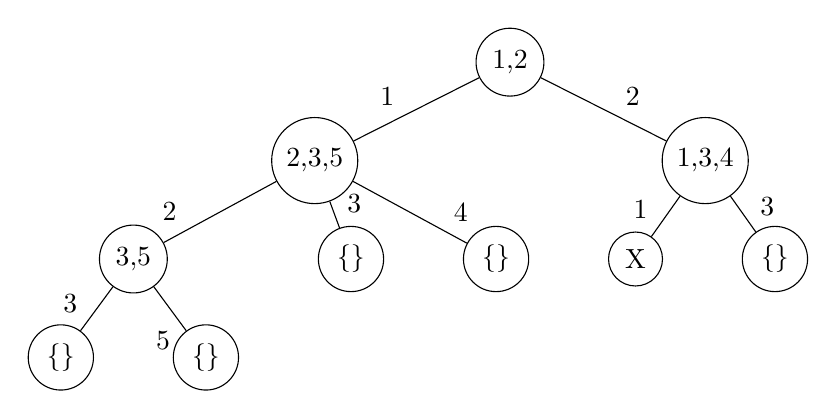
\begin{tikzpicture}[every tree node/.style={draw,circle},
					level distance=1.25cm,sibling distance=1cm,
					edge from parent path={(\tikzparentnode) -- (\tikzchildnode)}]
					\Tree
					[.1,2
					\edge node[auto=right,pos=.6] {$1$};
					[.2,3,5 
					\edge node[auto=right,pos=.8] {$2$};
					[.3,5 
					\edge node[auto=right,pos=.8] {$3$};
					[.{$\{\}$} ]
					\edge node[auto=right,pos=.8] {$5$};
					[.{$\{\}$} ]    	
					]
					\edge node[auto=left,pos=.8] {$3$};
					[.{$\{\}$} ]
					\edge node[auto=left,pos=.8] {$4$};
					[.{$\{\}$} ]
					]
					\edge node[auto=left,pos=.6] {$2$};
					[.1,3,4
					\edge node[auto=right,pos=.8] {$1$};
					[.X ]
					\edge node[auto=left,pos=.8] {$3$};
					[.{$\{\}$} ]
					]
					]
					\end{tikzpicture}
					\caption{Early Termination trong HST Explanation \label{overflow}}
\end{figure}

Chúng ta bắt đầu di chuyển root node với tập $\{1,2\}$ là các phát biểu đầu tiên tìm được trong $O$ chứng minh được $O$ $\models$ $\alpha$, thực hiện tương tự các bước đã được miêu tả ở trên ta thu được node $\{3,5\}$ là các phát biểu giải thích cho $O$ $\models$ $\alpha$, tới lúc này ta có thể thấy tập chứ đường đi theo cạnh từ node $\{3,5\}$ tới root node là $P_{1}=\{2,1\}$. Nhìn về phía bên phải ta phát hiện khi mở rộng cạnh từ node $\{1,3,4\}$ ta thu được đường đi về root node là $P_{2}=\{1,2\}$, ta thấy $P_{1} \equiv P_{2}$ do vậy nên khi dán nhãn cho node kế tiếp (được đánh dâu \xmark cho \textit{closed} node) chúng ta sẽ bỏ $\{1,2\}$ khỏi $O$ để được $O^{'}=\{3,4,5\}$, sẽ có một node giống y như node $\{3,5\}$ sẽ xuất hiện lần nữa ở node kế tiếp này nên việc kết thúc ở đây là cần thiết vì chúng ta sẽ tiếp kiệm được việc kiểm tra lại $\{3,5\}$ như ở bên trái.

\paragraph{Justification Reuse} - Cách quan trọng thứ hai để tối ưu là sử dụng lại các kiểm chứng. Trong phiên bản không tối ưu sử dụng ở ví dụ ontology $\beta$ ở trên, kiểm chứng được tìm ra nhờ các giải thuật Blackbox hay Glassbox cho từng node $v$ được thêm vào cây. Kiểm chứng hay tập các phát biểu được sử dụng để dán nhãn $v$, được tính toán dựa trên $O \backslash S$, với $S$ là tập các nhãn trên đường đi từ $v$ về root node. Thay vì dùng Glassbox hay Blackbox để tính $J$ trong $O \backslash S$, chúng ta có thể làm theo cách sau: nếu HST chứa vài node khác $v^{'}$ mà được dán nhãn với kiểm chứng $J$, và $S$ không giao (có phần tử chung) với $J$ thì $J$ có thể được sử dụng làm nhãn cho $v$. Lý do là vì khi $J\subseteq$ $O$ và $S\cap J = \emptyset$ thì sẽ tồn tại trường hợp $J\subseteq O \backslash S$, từ đó $J$ được tính như một kiểm chứng cho để có thể dán nhãn $v$. Sử dụng lại các phát biểu chứng minh (hay kiểm chứng) sẽ giúp tiết kiệm nhiều lời gọi hàm không cần thiết tới Blackbox hoặc Glassbox từ đó tăng được hiệu năng.
\\
\paragraph{Kết luận} Tính năng vừa trình bày \textit{Tìm tất cả các giải thích cho kết quả suy luận}, kĩ thuật \textit{Axiom Pinpoint} và \textit{BlackBox} được đã được áp dụng trong thư viện lặp trình OWL-API \cite{owlapi} sẽ được chúng em giới thiệu trong chương kế.


\chapter{Các thư viện lập trình OWLAPI, Pellet Reasoner, SWRLAPI và Vaadin framework sử dụng trong ứng dụng}
\paragraph{Giới thiệu} Trong chương này, chúng em xin giới thiệu khái quát qua các thư viện lập trình (API) và framework được sử dụng để xây dựng chương trình. Các thư viện sử dụng gồm có OWLAPI \cite{owlapi}, SWRLAPI \cite{swrlapi}, Pellet \cite{pellet}, Google Guava EventBus và thành phần giúp tạo nên giao diện người dùng của ứng dụng - Vaadin Framework. Đầu tiên xin được giới thư viện lập trình OWL-API.
\section{Thư viện lập trình OWLAPI}
Thư viện lập trình Ontology Web Language là một thư viện mã nguồn mở (phát hành dưới 2 giấy phép \textbf{LGPL} và \textbf{Apache}) \cite{owlapi} được viết bằng JAVA với mục đích hỗ trợ các lập trình viên phát triển các ứng dụng có liên quan đến OWL2 Ontology. Tính đến thời điểm hiện tại thư viện đã được phát triển đến phiên bản 4.0 - cũng là phiên bản được sử dụng trong ứng dụng của chúng em.
%Thư viện có các thành phần chính như sau: 
%\begin{itemize}
%\item API để tương tác với các thành phần của OWL 2 được đề cập trong chương 2.
%\item Renderer và Parser (dùng đọc và ghi OWL 2 Ontology) nhiều dạng cú pháp khác nhau đã đề cập ở chương 2 như \textit{RDF/XML}, \textit{OWL/XML}, \textit{OWL Functional Syntax}, \textit{Manchester OWL Syntax} và \textit{Turtle}.
%\item Reasoner Interfaces cho các reasoners khác nhau hỗ trợ cho việc suy luận.
%\end{itemize}
%Dưới đây là danh sách các Ontology Reasoner được hỗ trợ trong phiên bản 4.0:
%\begin{itemize}
%\item FaCT++ 
%\item Hermit
%\item Pellet \cite{pellet}
%\item JFact 
%\end{itemize}
%\begin{table}[h]
%	\centering
%	\begin{tabular}{|l|l|p{4cm}|}
%		\hline
%		Thành phần OWL 2 		& Đối tương trong OWL-API 		& Thừa kế từ đối tượng (OWL-API) \\
%		\hline
%		Ontology 				& OWLOntology 					& OWLObject, HasDirectImports,...  \\ 
%		\hline
%		Entity 					& OWLEntity 					& OWLObject,...  \\
%		\hline
%		Class 					& OWLClass 						& OWLClassExpression, OWLEntity, ...   \\		
%		\hline
%		ObjectProperty 			& OWLObjectProperty 			& OWLProperty, OWLEntity, ...   \\		
%		\hline
%		DataProperty 			& OWLDataProperty 				& OWLProperty, OWLEntity, ...   \\
%		\hline
%		NamedIndividual 		& OWLNamedIndividual			& OWLLogicalEntity, OWLEntity, ...  \\
%		\hline
%		Datatype 				& OWLDatatype 					& OWLDataRange, OWLPropertyRange, ...   \\
%		\hline
%		Property 				& OWLProperty 					& OWLLogicalEntity, OWLEntity   \\
%		\hline
%		ClassExpression			& OWLClassExpression			& OWLObject, OWLPropertyRange   \\
%		\hline
%		ObjectUnionOf			& OWLObjectUnionOf				& ClassExpression, ...\\
%		\hline
%		ObjectIntersectionOf	& OWLObjectIntersectionOf		& ClassExpression, ... \\
%		\hline
%		ObjectAllValuesFrom		& OWLObjectAllValueFrom		& ClassExpression, ... \\
%		\hline
%		ObjectSomeValuesFrom	& OWLObjectSomeValuesFrom		& ClassExpression, ... \\
%		\hline
%	\end{tabular}
%	\caption{Các đối tượng OWL2 trong OWL-API\label{overflow}}
%\end{table}
Trong thư viện OWL-API, có nhiều đối tượng được xây dựng dựa trên cấu trúc phân lớp của một OWL2 Ontology, tương tự các thành phần đã được chúng em trình bày trong chương 2. Dưới đây là bảng liệt kê một số thành phần mà OWL-API đã xây dựng dựa trên mô tả trong chương 2 (chi tiết hơn ở trong \cite{owl2spec} và mã nguồn (source code) của OWL-API \cite{owlapi}). Trên đây chỉ là một vài thành phần, mọi thành phần OWL2 được trình bày trong chương 2 đều được OWL-API xây dựng thành các đối tượng class, interface trong JAVA để phục vụ cho việc lập trình. Tuy nhiên để tương tác với một kiến trúc đối tượng lớn và phức tạp như 1 ontology cần có cách thức chuyên dùng cho việc này là Visitor Pattern.
\subsection{Visitor Pattern}
\begin{figure}[h!]
	\centering
	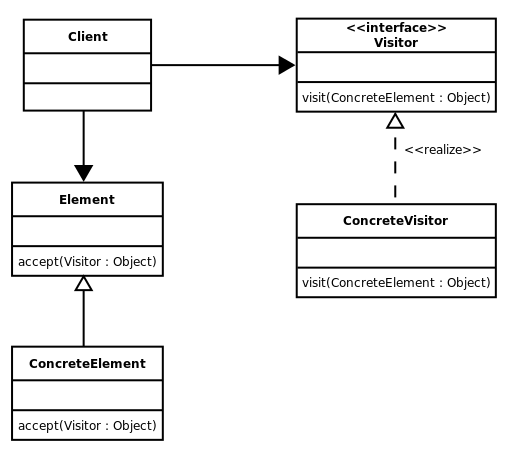
\includegraphics[width=110mm]{Figures/visitor_diagram.png}
	\caption{Visitor Diagram\label{overflow}}
\end{figure}
\paragraph{Khái quát} Trong lập trình hướng đối tượng và phát triển ứng dụng, Visitor Pattern hay Visitor Design Pattern là một cách để tách biệt một giải thuật ra khỏi cấu trúc của đối tượng mà nó đang xử lý. Nhờ sự tách biệt này, chúng ta có khả năng thêm một tính năng mới cho đối tượng mà không cần phải sửa đổi cấu trúc của đối tượng đó. Lấy ví dụ một visitor trong thư viện OWL-API là \textit{OWLClassExpressionVisitor}, chúng ta đã biết bên dưới có rất nhiều đối tượng thừa kế từ OWLClassExpression (mô tả lớp) như OWLObjectUnionOf, OWLObjectIntersectionOf, OWLClass, OWLObjectAllValueFrom, OWLObjectSomeValuesFrom,... Chúng ta xem qua các đoạn code sau :
\begin{verbatim}
// visitor interface
public interface OWLClassExpressionVisitor {
     public void visit(OWLClass cls);
     public void visit(OWLObjectUnionOf union);
     ...
}
// Lớp visitor
public class OWLClassExpressionVisitorImpl 
                 implements OWLClassExpressionVisitor {
    public void visit(OWLClass cls) {
        System.out.println("Lớp:" + cls.toString()); // (4)
    }
    public void visit(OWLObjectUnionOf union) {
        // Hàm getOperands trả về các mô tả lớp trong phát biểu unionOf
        for(OWLClassExpression ce: union.getOperands()) {
           ce.accept(this); // (2), (2')
        }
	}
	...
}
// Interface OWLClassExpression
public interface OWLClassExpression {
    public void accept(OWLClassExpressionVisitor visitor);
}
// Lớp OWLObjectUnionOf thừa kế từ OWLClassExpression
public class OWLObjectUnionOfImpl implements OWLClassExpression {
	public void accept(OWLClassExpressionVisitor visitor) {
    	visitor.visit(this); // (1)
    }
    ...
}
// Lớp OWLClass thừa kế từ OWLClassExpression 
public class OWLClass implements OWLClassExpression {
    public void accept(OWLClassExpressionVisitor visitor) {
        visitor.visit(this); // (3)
    }
    ...
}
// Hàm main 
public void main(String[] args) {
   OWLDataFactory factory = OWLManager.getOWLDataFactory();
   OWLClass car = factory.getOWLClass("a:Car");
   OWLClass bike = factory.getOWLClass("a:Bike");
   OWLObjectUnionOf union = factory.getOWLObjectUnionOf(car, bike);
   OWLClassExpressionVisitor visitor = new OWLClassExpressionVisitorImpl();
   union.accept(visitor);                                       
}
// Output của hàm main sẽ là 
Lớp: a:Car
Lớp: a:Bike
\end{verbatim}
Đối tượng \textit{OWLDataFactory} sẽ được trình bày ở mục sau, chúng ta có thể hiểu hàm \textit{main} như sau factory tạo ra 2 đối tượng OWLClass là car, bike tương đương với 2 lớp trong OWL2 a:Car, a:Bike, tiếp đó factory tạo ra một đối tượng union tương đương \textit{ObjectUnionOf( a:Car a:Bike )} trong OWL2. Cuối cùng ta sử dụng cho union.accept(visitor) thì thứ tự gọi hàm cho tới khi in ra từng dòng output là (1),(2),(3) và (4). 
\\
Đây chính là cách một \textit{visitor} hoạt động, thư viện OWL-API sử dụng lặp đi, lặp lại rất nhiều lần các interface visitor cho nhiều tác vụ khác nhau từ parser (dịch raw text thành cú pháp của OWL 2), renderer(dùng đọc các thành phần của ontology) như ví dụ trên qua các interface như OWLObjectVisitor, OWLDatatypeVisitor,... hoặc đọc và dịch SWRL Rule qua interface SWRLObjectVisitor. Chúng em cũng sử dụng \textit{Visitor Pattern} rất nhiều lần trong ứng dụng của mình để thực hiện nhiều tác vụ tương tự.
\subsection{Các hàm và đối tượng quan trọng cần biết khi sử dụng OWL-API}
\subsubsection{OWLOntologyManager}
Đây là thành phần đầu tiên cần khởi tạo trước khi chúng ta muốn nạp hay tạo một OWL2 Ontology nào, chức năng quản lý các ontology được khởi tạo, nạp. Cú pháp:
\begin{verbatim}
OWLOntologyManager modelManager = OWLManager.createOWLOntologyManager();
OWLOntolgoy ont  = modelManager.loadOntologyFromOntologyDocument(ontologyIRI);
OWLOntolgoy ont2  = modelManager.createOntology(ontologyIRI);
\end{verbatim}
\subsubsection{OWLDataFactory}
OWLDataFactory hoạt động giống như một nhà máy tạo ra tất cả đối tượng các thành phần trong OWL2 mô tả trong \cite{owl2spec} và chương 2. Cú pháp:
\begin{verbatim}
 OWLDataFactory factory = modelManager.getOWLDataFactory();
 OWLClass car = factory.getOWLClass("a:Car")
 OWLObjectProperty hasId = factory.getObjectProperty(":hasId",prefixManager);
\end{verbatim}
\subsubsection{PrefixManager}
Có chức năng quản lý các OntologyIRI, OntologyID, VersionIRI. Cú pháp:
\begin{verbatim}
// Khởi tạo PrefixManger và set IRI mặc định là "DemoIRI"
PrefixManager pm = new DefaultPrefixManager(null, null, "DemoIRI#");
\end{verbatim}
\subsubsection{OWLOntology}
Là một bản mapping của OWL2 ontology thành các đối tượng trong Java, tất cả được lưu trong bộ nhớ (in-memory). Load ontology từ file nội bộ và URI:
\begin{verbatim}
String uri = "http://chuongdang.com/transport.owl";
File file = new File("./transport.owl");
OWLOntolgoy ont  = modelManager
                  .loadOntologyFromOntologyDocument(IRI.create(uri));
OWLOntolgoy ont2 = modelManager
                  .loadOntologyFromOntologyDocument(IRI.create(file));
\end{verbatim}
\subsubsection{EntitySearcher}
Static class \verb|EntitySearcher| cho phép truy vấn đến các cá thể trong OWL2 Ontology một cách nhanh nhất nếu chúng đã được khai báo. Ví dụ để tìm các mô tả lớp con của một lớp nào đó trong OWL 2 Ontology:
\begin{verbatim}
OWLOntology ont = modelManager.loadOntologyFromOntologyDocument(ontologyIRI);
OWLClass person = factory.getOWLClass("a:Person");
// Tìm các lớp con của person trong ontology "ont"
Collection<OWLCLassExpression> subClasses = 
			EntitySearcher.getSubClasses(person, ont);
			
\end{verbatim}
Lưu ý: Cần phân biệt các tính năng của \verb|EntitySearcher| với thành phần reasoner vì reasoner cũng có các hàm đảm nhiệm tính năng tương tự. EntitySearher chỉ tìm những phát biểu \textbf{đã} khai báo trong ontology, còn Reasoner tìm những phát biểu \textbf{được suy luận} ra từ dữ kiện của ontology.

\subsubsection{OWLObjectRenderer}
Đảm nhiệm khả năng ghi và biên dịch các thành phần của ontology từ IRI thành dạng vắng tắt, mỗi một dạng cú pháp sẽ có một đối tượng renderer khác nhau implements OWLObjectRenderer. Ví dụ cú pháp Manchester Syntax:
\begin{verbatim}
OWLObjectRenderer renderer = 
                  new ManchesterOWLSyntaxOWLObjectRendererImpl();
// Render ClassExpression
OWLObjectProperty buy = factory
                   .getOWLObjectProperty("http://vehicle.org#Buy");
OWLObjectSomeValuesFrom ce = factory.getOWLObjectSomeValuesFrom(buy, car);
System.out.println(renderer.render(ce));
// Output: Buy some Car <- Manchester Syntax
\end{verbatim}
Ngoài ra còn rất nhiều thành phần quan trọng mà chúng em sử dụng đến trong việc phát triển ứng dụng , chúng em sẽ trình bày trong chương sau khi nói về quá trình phát triển ứng dụng phát triển ontology trên web.
\section{Pellet Reasoner}
Như đã đươc nhắc đến nhiều lần trong báo cáo, suy luận được xem là một điểm đáng giá nhất của ngôn ngữ OWL2. Tuy nhiên, việc suy luận ra các phát biểu hàm ý rõ ràng không phải là một việc dễ dàng nếu chúng ta thực hiện thủ công bằng cách đọc và hiểu các phát biểu như đã làm trong chương 2. Sử dụng Reasoner sẽ làm cho công việc suy ra các mảnh thông tin ẩn chứa bên trong Ontology trở nên dễ dàng hơn rất nhiều, có rất nhiều reasoner được phát triển để thực hiện tác vụ này. Trong số đó Pellet \cite{pellet} là một thư viện tối ưu nhất và  một ưu điểm đặc biệt hơn nữa là khả năng suy luận từ những SWRL Rule.

Pellet được phát triển bởi Clark và Parsia \cite{repair} \cite{axiomPinpoint} là những tác giả của kỹ thuật BlackBox, AxiomPinpoint và giải thuật HST được trình bày trong chương \textit{Tính nhất quán của Ontology}, đồng tác giả của các module explanation và modularity trong thư viện OWL-API vừa nêu. Vì vậy, không khó hiểu khi Pellet và OWL-API hoạt động rất tốt khi kết hợp với nhau.
\\
Pellet Reasoner được phát hiện theo giấy phép open source (AGPL) và phiên bản được chúng em sử dụng là 2.2.2, phiên bản mới hơn 3.0 là phiên bản thương mại hóa.
\\
Sau đây, chúng em xin trình bày một ví dụ về cách sử dụng Pellet với OWL-API:
\begin{verbatim}
// Có ontology sau
Declaration(Class(a:Person))
Declaration(NamedIndividual(a:Nguyen))
Declaration(DataPropery(a:HasAge))
DataPropertyAssertion(a:HasAge a:Nguyen "22"^^xsd:int)
// Người có số tuổi sẽ đều là người ~ Person
DataPropertyDomain(a:HasAge a:Person)
...
OWLOntology ontology = // load từ IRI 
OWLNamedIndividual Nguyen = factory.getOWLNamedIndividual("a:Nguyen"); 
OWLReasonerFactory reasonerFactory = PelletReasonerFactory.getInstance();
OWLReasoner reasoner = 
      reasonerFactory.createReasoner(ontology, new SimpleConfiguration());
reasoner.precomputeInferences();
// Tìm xem Nguyen thuộc những lớp nào
Set<OWLClass> hiddenMeaning = reasoner
      .getTypes(Nguyen, false).getFlattened();
hiddenMeaing.forEach(cls -> System.out.println(cls));
// Output
a:Person
a:Thing
\end{verbatim}
Xin được nhắc lại ở trên, \verb|EntitySearcher| cũng có tính năng |getTypes| tương tự tuy nhiên nó sẽ không in ra output nào trong trường hợp này vì nó chỉ tìm những phát biểu đã \textbf{khai báo} trong ontology, không giống như Reasoner là tìm những phát biểu được suy luận ra. Lưu ý: Nếu trong \verb|getTypes| trong ví dụ trên nếu ta để \verb|true| thì kết quả sẽ không có \textit{a:Thing}, \verb|false| có nghĩa là tìm luôn những lớp bên mà \textit{a:Person} là lớp con của chúng, \verb|true| thì ngược lại.
\\
Trên đây chỉ là một ví dụ đơn giản về cách sử dụng của reasoner, thầy cô và bạn đọc có thể tham khảo thêm ở \cite{pellet}.

\section{SWRL API}
SWRL API được xây dựng bởi nhóm phát triển dự án Protege \cite{protege} với mục tiêu tổ chức các SWRL Rule theo tên nhằm dễ dàng quản lý, đồng thời họ cũng giới thiệu SQWRL \cite{swrlapi} một ngôn ngữ truy vấn dành cho Ontology. Trong nội dung báo cáo, chúng em chỉ sử dụng tính năng SWRL Rule của SWRLAPI các tính năng còn lại có thể được tham khảo tại \cite{swrlapi}. Các tính năng mà chúng em sử dụng gồm render, parse SWRL Rule và thêm/xóa SWRL Rule theo tên của chúng. Một ví dụ nhanh về cách sử dụng API này với OWL-API:
\begin{verbatim}
OWLOntology ont = // load ontology ../
// Convert OWLOntology -> SWRLAPIOWLOntology
SWRLAPIOWLOntology SWRLOnt =  SWRLAPIFactory.createOntology(ont);
   
SWRLAPIRenderer ruleRenderer = 
                  new DefaultSWRLAPIRenderer(SWRLOnt);
// Rule được tự động add và cập nhật trong đối tượng OWLOntology                  
SWRLAPIRule apiRule = SWRLOnt.createSWRLRule(
                 "RuleName", "Driver(?x) -> Person(?x)");
// Render rule -> string
System.out.println(ruleRenderer.render(apiRule));
\end{verbatim}

\section{Vaadin Framework }
\paragraph{Giới thiệu} Vaadin Framework là nền tảng xây dựng một ứng dụng web trên Java được thiết kế giúp tạo ra một ứng dụng web chất lượng cao một cách dễ dàng nhất - tập trung chủ yếu vào one-page web application. Không giống như những framework web hiện nay đòi hỏi lập trình viên phải có kiến thức về HTML5, Javascript và ít nhất một ngôn ngữ back-end. Vaadin giúp chúng ta tạm quên việc đi việc phải viết các client Javascript hay từng dòng HTML để xây dựng giao diện người dùng - nói cách khác nó làm cho công việc phát triển front-end trở nên cực kì đơn giản, dễ hình dung nhất là việc phát triển một ứng dụng web trên Vaadin cũng tương tự khi chúng ta phát triển một ứng dụng desktop thông thường với các công cụ Java như AWT, Swing, hay SWT hoặc window form với C\verb|#|(C-Sharp).  Với Vaadin, để phát triển được toàn bộ một ứng dụng, ngôn ngữ duy nhất chúng ta cần nắm đó là Java. Một ví dụ minh họa về tính đơn giản trong khi sử dụng Vaadin:
\begin{verbatim}
 Button button = new Button("Demo");
 button.addClickListener( new ClickListener() {
    layout.addComponent(new Label("The button was clicked"));
 }
\end{verbatim}
Đây là kết quả:
\begin{figure}[H]
 	\centering
 	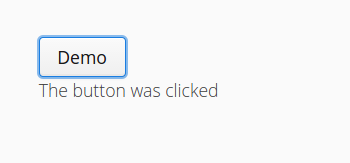
\includegraphics[width=80mm]{Figures/vaadin_democlick.png}
 	\caption{Vaadin Demo Click\label{overflow}}
\end{figure}
Thử nhìn lại nếu chúng ta xây dựng cùng chức năng trên dù là thủ công hay sử dụng các framework Web thông thường thì đều cần phải có một client script đảm nhận việc bắt sự kiện click của người dùng ở browser (front-end) và truyền nó lên server, ngay khi server nhận được (phải có đoạn code ở server "back-end" để xử lý thông tin click truyền lên từ browser), server sẽ trả về thông báo "The button was clicked", rồi front-end javascript phải thêm hay chèn một đoạn text "The button was clicked" vào HTML. Với Vaadin tác vụ vừa mô tả được thực hiện bằng đoạn code trên một cách đơn giản và dễ hiểu hơn rất nhiều.
\subsection{Kiến trúc}
Vaadin hỗ trợ 2 mô hình lập trình: client và server. Mô hình lập trình phía server mạnh mẽ hơn. Mô hình lập trình phía server đảm nhận phần giao diện trên trình duyệt và giao tiếp AJAX giữa trình duyệt và server - hay nói cách khác các giao tiếp giữa server-client nhằm hỗ trợ những thao tác của người dùng đã được xử lý bởi framework và được cài đặt vào bên trong các \textit{Component} của Vaadin. Trong phạm vi ứng dụng mà chúng em xây dựng chỉ sử dụng những thành phần server - chỉ sử dụng các \textit{Component} mà Vaadin cung cấp, cộng với một vài plugin (được viết sẵn cho Vaadin) từ Vaadin Directory \cite{vaadindirectory} để giúp việc phát triển nhanh chóng hơn. 
\\
Hình sau mô tả kiến trúc cơ bản của một ứng dụng web trên Vaadin Framework. Kiến trúc ứng dụng phía server bao gồm nền tảng server (Server-side framework) và hệ thống phía client (Client-side engine). 
\begin{figure}[ht!]
	\centering
	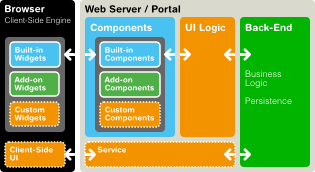
\includegraphics[width=100mm]{Figures/vaadin_architecture0.png}
	\caption{Kiến trúc của Vaadin\label{overflow}}
\end{figure}

\subsubsection{Web Server}
\begin{description}
\item[Components] Các \textit{Built-in Components}, \textit{Add-on Components} đều là những thành phần được xây dựng sẵn bởi Vaadin hoặc được cung cấp dưới dạng các add-on từ Vaadin Directory \cite{vaadindirectory} nhằm giúp việc phát triển UI nhanh chóng hơn. Chúng đảm nhiệm back-end code để giao tiếp với các \textit{Built-in Widgets}, \textit{Add-on Widgets} ở phía browser (client side).
\item[UI Logic, Service và Custom Components] là những phần mà lập trình viên phải tự viết code để cài đặt các tác vụ tương tác mà họ mong muốn, tuy nhiên Vaadin cũng cung cấp các abstract class, interface để hỗ trợ việc này. 
\item[Back-end] Trong một ứng dụng thông thường thì đây chính là nơi để xử lý giao tiếp với các đối tượng trong cơ sở dữ liệu - nơi thực hiện các thao tác Create Read Update Delete (CRUD).
\end{description}
\subsubsection{Client-Side Engine}
\begin{description}
\item[Built-in Widgets] Đây chính là thành phần Client-side của \textit{Built-in Components} đảm nhiệm bắt các sự kiện của người dùng với browser và giao tiếp với các \textit{Built-in Components} ở server.
\item[Add-on Widgets] là client-side của \textit{Add-on Components}.
\item[Custom-Widgets] là client-side của \textit{Custom Components}.
\end{description}
Toàn bộ các thành phần ở Client-side Engine đều được xây dựng bằng JavaScript. Đây là một ưu thế so với các nền tảng trên Flash, Java Applets hay các plugins khác. Vaadin dựa trên sự hỗ trợ của Google Web Toolkit cho nhiều trình duyệt khác nhau, nên lập trình viên không cần lo lắng về sự tương thích của các trình duyệt cho ứng dụng của mình.
\\
Như đã nói ở trên, không giống với các framework web khác là tách biệt front-end và back-end thành 2 phần riêng biệt, Vaadin làm điều ngược lại đó là đem cả hai thành phần đó tích hợp vào \textit{Vaadin Components}, ở hình trên chúng ta sẽ thấy một \textit{Vaadin Component} sẽ gồm một \textit{Widget} ở client-side  và một \textit{Component} tương ứng ở server side. Phân tích ví dụ Demo Click ở bên trên :
\begin{itemize}
\item \textbf{Vaadin Component} chính là một Vaadin Component.
\item \textbf{UILogic} chính là \textit{layout.addComponent(new Label("The button was clicked"));}
\end{itemize}

Tóm tắt lại, Vaadin cung cấp sẵn gần như đầy đủ mọi thành phần UI chúng ta cần để phát triển một ứng dụng web tương tác tốt với người dùng một cách nhanh chóng và tiện lợi. Chúng ta sẽ giảm bớt được công việc khi phải viết Javascript, HTML cho cliend-side khi sử dụng các Vaadin UI Components.
\\
Tuy là tích hợp mọi thứ vào UI components của mình, Vaadin tách biệt UI Logic với các thiết kế giao diện. Điều này đồng nghĩa bên cạnh một giao diện mặc định rất tốt của Vaadin chúng ta có thể thiết kế giao diện một cách dễ dàng thông qua các file CSS hoặc cũng có thể tự định nghĩa HTML Template cho riêng mình \textsuperscript{*}. 
{\let\thefootnote\relax\footnotetext{*\textit{
			Vaadin Theme: https://vaadin.com/book/-/page/themes.html}}
}


%Trong hình sẽ cung cấp những thông tin chi tiết hơn về các đối tượng mà Vaadin xây dựng nhằm phục vụ cho việc thực thi các yêu cầu từ client-server và ngược lại. Mô hình trên còn được gọi là kiến trúc Server-driven Development.

\subsection{Vaadin UI Components}
Như đã được nhắc đến nhiều lần trong mục trước, Vaadin UI Component chính là những thành phần tạo nên Vaadin và đơn giản hoá rất nhiều công việc khi chúng ta phát triển ứng dụng web. Dưới đây chúng em xin được nêu lên những thành phần đáng chú ý nhất. Đầu tiên xin giới thiệu thành phần quan trong nhất.

\subsubsection{User Interface} 
\paragraph{Chức năng} Ứng dụng Vaadin cung cấp một giao diện người dùng để lập trình viên có thể mở rộng ra và phát triển các chức năng mà mình mong muốn. Về mặt kĩ thuật, thành phần này sẽ được đảm nhiệm bởi các đối tượng thừa kế từ \textit{com.vaadin.ui.UI} trong source code.
\paragraph{Nhiệm vụ} Khởi tạo lớp UI, từ đây lớp UI sẽ đảm nhiệm các công việc như nạp tất cả UI Components được khai báo bên trong, cài đặt các event listener để tiếp nhận thao tác từ người dùng. Cuối cùng UI được load lên trình duyệt bằng URL, hoặc được nhúng 
vào bất kì trang HTML nào \cite{vaadinarchitecture}.


\subsection{Các UI Component đáng chú ý}
Dưới đây chúng em xin được liệt kê các Components được chúng em sử dụng nhiều trong việc phát triển ứng dụng OWLEditor.
\begin{figure}[h!]
	\centering
	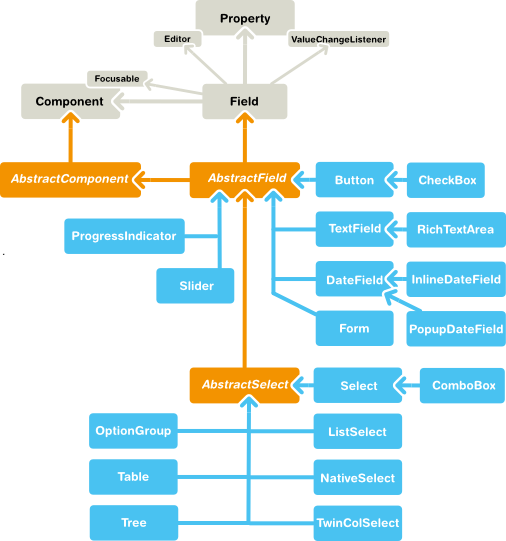
\includegraphics[width=120mm]{Figures/vaadin_architecture1.png}
	\caption{Các UI Components của Vaadin\label{overflow}}
\end{figure}
\subsubsection{Layout}
Vaadin cung cấp nhiều dạng layout khác nhau để hỗ trợ việc tổ chức các components bên trong một cách khoa học, gọn gàng. \cite{vaadinbook}
\begin{description}
\item[HorizontalLayout] tổ chức các components theo chiều ngang, các component được sắp xếp từ trái qua phải.
\item[VerticalLayout] tổ chức các components theo chiều dọc, các component được sắp xếp từ trên xuống.
\item[AbsoluteLayout] tổ chức các components theo đúng vị trí tuyệt đối được khai báo.
\item[CssLayout] tổ chức các components theo định nghĩa từ các file css tương ứng. Đây là cách giúp chúng ta có thể tuỳ chỉnh tối đa bố cục của ứng dụng so với các layout trên.
\end{description} 
\subsubsection{Field Component}
Là những components được thừa kế từ \verb|AbstractField| với chức năng là xử lý các tác vụ input từ người dùng.
\begin{description}
\item[Button] Đảm nhiệm tính năng click từ người dùng, hành động click được xử lý bởi Button.ClickListener và ClickEvent.
\item[CheckBox] Component đảm nhiệm đánh dấu tick từ người dùng, sự kiện được xử lý bởi ValueChangeListener và ValueChangeEvent.
\item[TextField] Đảm nhiệm việc nhập liệu từ người dùng, sự kiện là TextChangeEvent được xử lý bởi TextChangeListener. Hỗ trợ kiểm tra đánh giá input (Validation) cho dữ liệu được nhập vào qua AbstractValidator.
\end{description} 
\subsubsection{Select Component}
Là những components được thừa kế từ \verb|AbstractSelect| với chức năng chính là hiển thị các Data Model (sẽ được đê cập ngay ở mục sau) ra thành các dạng sau.
\begin{description}
\item[Tree] Component cho phép hiển thị Data Model thành dạng cây (ví dụ như cây thư mục), hỗ trợ nhiều tương tác như chọn, thêm, xóa node trên cây.
\item[Table] Component cho phép hiện thị Data Model thành dạng bảng (ví dụ dữ liệu bảng từ SQL Table), hỗ trợ các thao tác như chọn, thêm , xóa dòng trên bảng.
\item[ListSelect] Hiển thị các Data Model theo dạng danh sách, hỗ trợ các thao tác chọn từng dòng, nhiều dòng, thêm dòng và xóa dòng trong danh sách.
\item[ComboBox] Hiện thị các Data Model theo dạng danh sách sổ xuống, hỗ trợ các thao tác như chọn một, thêm dòng mới trong danh sách.
\end{description}
\subsubsection{TabSheet}
\hspace{0.05\textwidth} Tabsheet là một thành phần của Vaadin, là một không gian đa thành phần (multicomponent), có thể chứa nhiều thành phần con bên trong, cho phép chuyển đổi giữa các thành phần bằng cách thay đổi "tab". Các "tab" được sắp xếp như một thanh công cụ luôn nằm ở vị trí cao nhất trong Tabsheet. Khi các "tab" được thay đổi qua lại, thành phần chính của tab đó sẽ trở thành vùng hiển thị chính trên giao diện. Nếu có nhiều tab trong thanh công cụ, các nút điều hướng sẽ được tự động hiển thị. Mỗi tab được xem như là một đối tượng Tab, dùng để quản lý tiêu đề, icon và các thuộc tính khác như ẩn, hiện 
\\
Khi click một tab, Vaadin sẽ kích họat sự kiện TabSheet.SelectedTabChangeEvent, có thể 
được xử lý với interface TabSheet.SelectedTabChangeListener. Thông qua phương thức 
getTabSheet() để lấy được đối tượng tabsheet, và dùng phương thức getSelectedTab() để biết được tab đã được người dùng lựa chọn.

\subsection{Data Model}
Vaadin Data Model cho phép các View (UI components) truy xuất tới dữ liệu một cách trực tiếp, bằng cách cung cấp một interface chuẩn cho mọi loại dữ liệu. Mô hình này cho phép binding các view trực tiếp đến dữ liệu để hiển thị, và cập nhật sự thay đổi ngay lập tức khi dữ liệu được chỉnh sửa. Trong mô hình này có 3 cấp độ cấu trúc khác nhau : property, item và container.
\\
Cần lưu ý rằng Data Model không định nghĩa cách mô tả dữ liệu, mà chỉ định nghĩa interfaces cho việc binding dữ liệu đến các View. Điều này cho phép dữ liệu trong Data Model không bị giới hạn, có thể là các object Java thông thường, đường dẫn hệ thống, hoặc có thể là các câu truy vấn cơ sở dữ liệu.
\\
Data Model được sử dụng rất nhiều trong các component của Vaadin, đặc biệt là các component thừa kế interface Field hoặc AbstractField được đề cập ở mục trên. Một điều thú vị đó là khi tương tác làm cho dữ liệu trong Data Model thay đổi thì dữ liệu hiển thị trên UI Component liên kết với Data Model sẽ tự động được cập nhật. Data Model được tổ chức thành 3 cấp độ khác nhau:
\begin{figure}[h!]
	\centering
	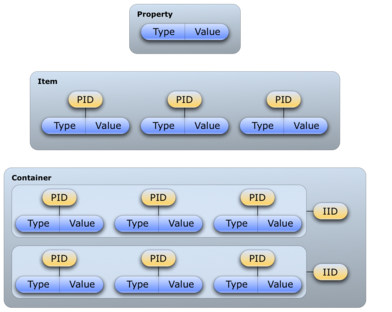
\includegraphics[width=100mm]{Figures/vaadin_datamodel.png}
	\caption{DataModel trong Vaadin\label{overflow}}
\end{figure}
\subsubsection{Properties}
Interface Property là thành phần cơ bản của Vaadin Data Model. Nó cung cấp cho đối tượng dữ liệu các phương thức đọc (get), ghi (set) cơ bản. Kiểu dữ liệu của một property có thể là bất kì lớp Java nào, và nó cũng hỗ trợ chuyển đổi giữa các kiểu dữ liệu.
\begin{itemize}
\item Phương thức setValue() dùng để ghi dữ liệu.
\item Phương thức getValue() dùng để đọc dữ liệu.
\end{itemize}
Các thay đổi của property sẽ kích hoạt sự kiện ValueChangeEvent, và được xử lý bằng ValueChangeListener. Truy xuất đến property bằng cách gọi phương thức getProperty() của event. Property thường không có định danh riêng. Chỉ khi chúng được chứa trong Item, chúng sẽ được định danh bằng các PID (Property Identifier). Tương tự, khi các Item được chứa trong Container, chúng sẽ có các định danh là các IID (Item Identifier). Mỗi component đều có một thuộc tính dùng để liên kết với nguồn dữ liệu được binding, sử dụng phương thức setPropertyDataSource() để thực hiện liên kết này.
\paragraph{Converter} Khi thực hiện binding, chúng ta sẽ gặp phải trường hợp kiểu dữ liệu của data khác với kiểu dữ liệu của component. Để giải quyết điều này, Vaadin cung cấp interface Converter, cho phép lập trình viên sử dụng để tạo ra các converter tuỳ theo mục đích sử dụng, để chuyển đổi kiểu dữ liệu của data sang kiểu dữ liệu hiển thị được của component. Vaadin cung cấp sẵn một vài converter thông dụng, như chuyển đổi giữa string và integer. Tuy nhiên trong ứng dụng OWLEditor, chúng em đã tự định nghĩa ra các Converter của mình để chuyển đổi giữa String và các đối tượng OWLEnity như OWLClass, OWLObjectProperty. Tất cả converter tự xây dựng được khuyến khich để trong ConverterFactory mà Vaadin cung cấp nhầm tự động phát hiện kiểu dữ liệu của MODEL và PRESENTATION để hệ thống tự động chọn converter thích hợp mà không cần cài đặt converter cho component.
\subsubsection{Item} Item được xem như một tập hợp dùng để chứa và quản lý các property. Mỗi property sẽ được gán định danh PID (Property Identifier) và được truy xuất đến bằng cách gọi phương thức getItemProperty() từ đối tượng Item. Item được xem như tương đương với một đối tượng cơ bản trong lập trình hướng đối tượng, tuy nhiên mở rộng hơn với khả năng xử lý được các sự kiện thay đổi liên quan tới nó. Khi các property trong Item bị thay đổi, Item kích hoạt sự kiện PropertySetChangeEvent được xử lý thông qua interface PropertySetChangeListener .
\subsubsection{Container}
Container là cấp cao nhất của mô hình dữ liệu Vaadin ( Vaadin Data Model ), chứa đựng và quản lý các item, trong các item lại chứa đựng và quản lý các property. Container hiển thị dữ liệu dưới dạng cấu trúc, như các dữ liệu thường thấy trong các bảng (Table), hay cây (Tree). Các item trong container được định dang bằng IID (Item Identifier), và các property trong item được định dang bằng PID (Property Identifier).

\chapter{Xây dựng UIT-OWL Editor}
\paragraph{Giới thiệu} Qua các chương trước, chúng em đã trình bày các cơ sở lý thuyết từ Semantic Web, Ontology Web Language và giới thiệu khái quát về OWL-API, Vaadin Framework- 2 công cụ chính xây dựng nên ứng dụng chỉnh sửa và phát triển Ontology trên Web mà chúng em tạm gọi là UIT-OWL Editor. Trong chương này, chúng em sẽ trình bày một cách chi tiết nhất có thể về quá trình xây dựng và phát triển nên ứng dụng này.
\section{UI của ứng dụng}
%\begin{figure}[h!]
%	\centering
%	\frame{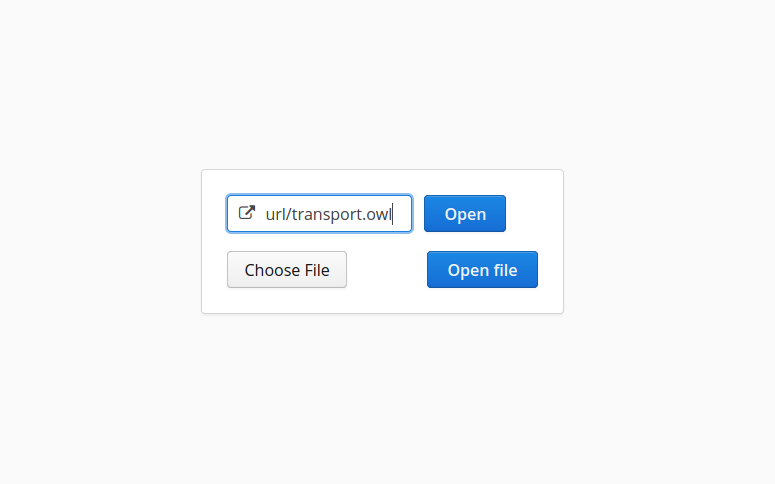
\includegraphics[width=100mm]{Figures/owleditor_entryview.png}}
%	\caption{EntryView của UIT-OWL Editor\label{overflow}}
%\end{figure}
\subsection{OWLEditorUI}
Lớp \textit{OWLEditorUI} thừa kế từ lớp \textit{UI} của Vaadin chính là User Interface của toàn bộ ứng dụng, hoạt động của lớp này tương tự miêu tả của chúng em ở chương trước khi giới thiệu về Vaadin. Chức năng của lớp này gồm:
\begin{enumerate}
	\item Chứa 2 View chính là EntryView và MainView.
	\item Cung cấp đối tượng \textit{OWLEditorKit} cho các UI Component sử dụng qua getter \textit{OWLEditorUI.getEditorKit} nhằm đảm bảo \textit{OWLEditorKit} chỉ khởi tạo 1 lần và chỉ liên kết đến 1 UI là \textit{OWLEditorUI}.
	\item Cung cấp đối tượng \textit{HttpSession} cho các UI Component qua getter \textit{OWLEditorUI.getHttpSession}.
	\item Cung cấp cơ chế reload để nạp ontology mới qua hàm \textit{updateContent}
	\item Cung cấp cơ chế xử lý sự kiện \textit{OWLEditorEventBus} nhằm xử lý các sự kiện cho ứng dụng.
\end{enumerate}
%
\subsection{Các view chính}
Ứng dụng UIT-OWLEditor chỉ gồm 2 View chính: 
\begin{description}
\item[Entry View] tương đương với lớp \textit{vn.edu.uit.owleditor.EntryView} trong mã nguồn, là nơi chúng tập nhập vào URL của file OWL2 Ontology hoặc tải file OWL2 Ontology với các định dạng được trình bày trong chương 2. Khi load được ontology \textit{EntryView} sẽ lưu đối tượng \textit{OWLEditorKit} lại trong \textit{HttpSession} phòng trường hợp người dùng mất kết nối với ứng dụng.
\begin{figure}[h!]
	\centering
	\frame{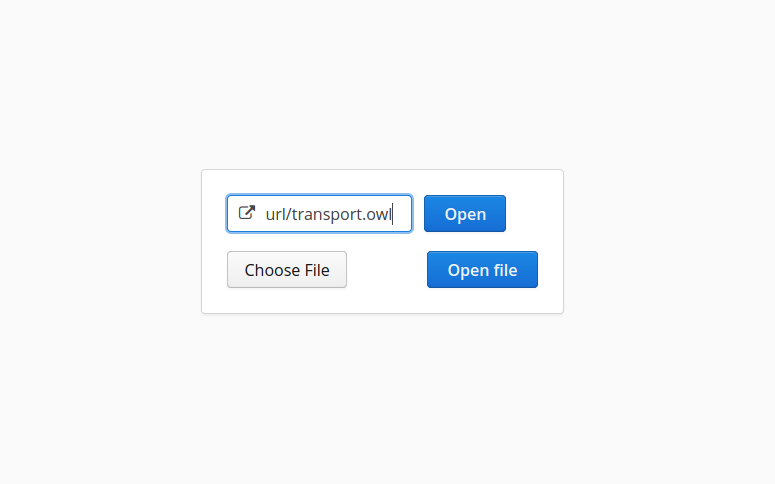
\includegraphics[width=100mm]{Figures/owleditor_entryview.png}}
	\caption{EntryView của UIT-OWL Editor\label{overflow}}
\end{figure}
\item[Main View] tương đướng với lớp \textit{vn.edu.uit.owleditor.MainView} trong mã nguồn,là giao diện chính của ứng dụng UIT-OWL Editor.
\end{description}
%
\subsection{Các tabsheet trong Main View}
Trong \textbf{MainView} sử dụng Component TabSheet các chứa các Tab tương ứng với các thực thể trong OWL2 Ontology, duy chỉ có 2 Tab cuối dùng để dùng làm demo tính năng phân loại là Tab Demo và Tab cuối cùng là Diagram dùng để vẽ các diagram, đồ thị về phân cấp các đối tượng trong OWL 2 Ontology.

% Class Tab
\subsubsection{Tab Classes} 
\begin{figure}[h!]
	\centering
	\frame{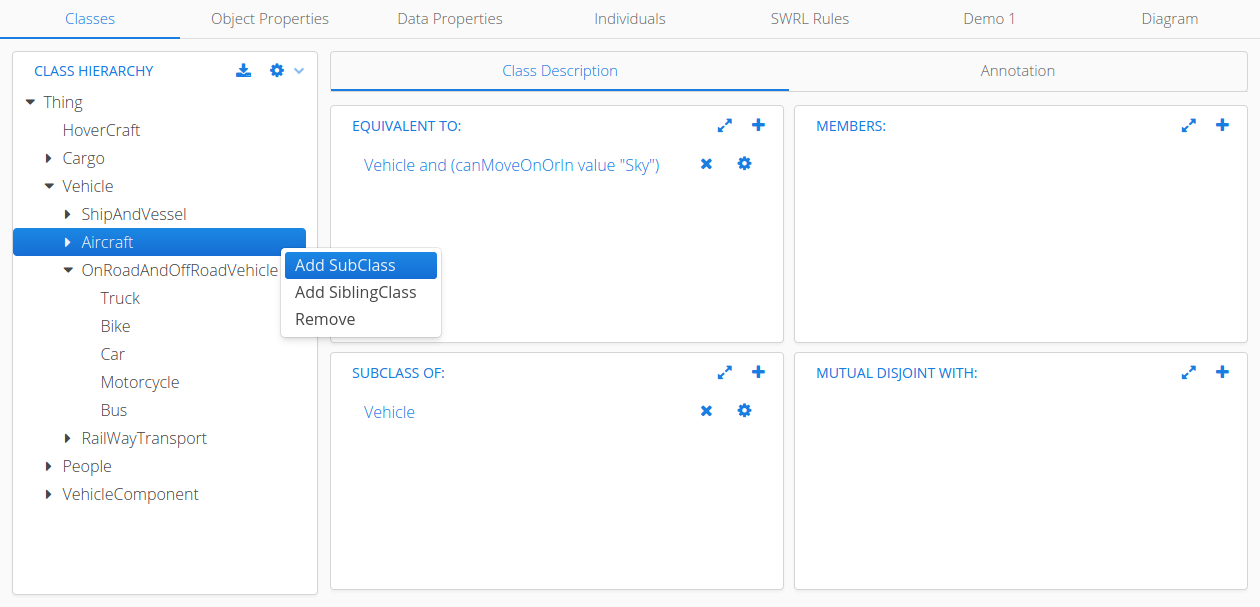
\includegraphics[width=145mm]{Figures/owleditor_classSheet.png}}
	\caption{Class Tab trong UIT-OWL Editor\label{overflow}}
\end{figure}
Tương ứng với lớp \verb|vn.edu.uit.owleditor.view.ClassesSheet| trong mã nguồn. Giao diện sử dụng HorizontalLayout của Vaadin gồm 
\begin{enumerate}
\item Panel bên trái là ClassHierachicalPanel có một cấu trúc dạng cây với các node chính là các lớp nằm trong OWL2 Ontology, với các chức năng thêm/xóa Sub/Sibling Class 
\item Các panel nhỏ bên phải được chứa trong lớp ClassExpressionPanelContainer, mỗ panel thể hiện một mô tả tương ứng với tên của panel đó.
\end{enumerate}	

% Object Property Tab
\subsubsection{Tab Object Properties}  
\begin{figure}[h!]
	\centering
	\frame{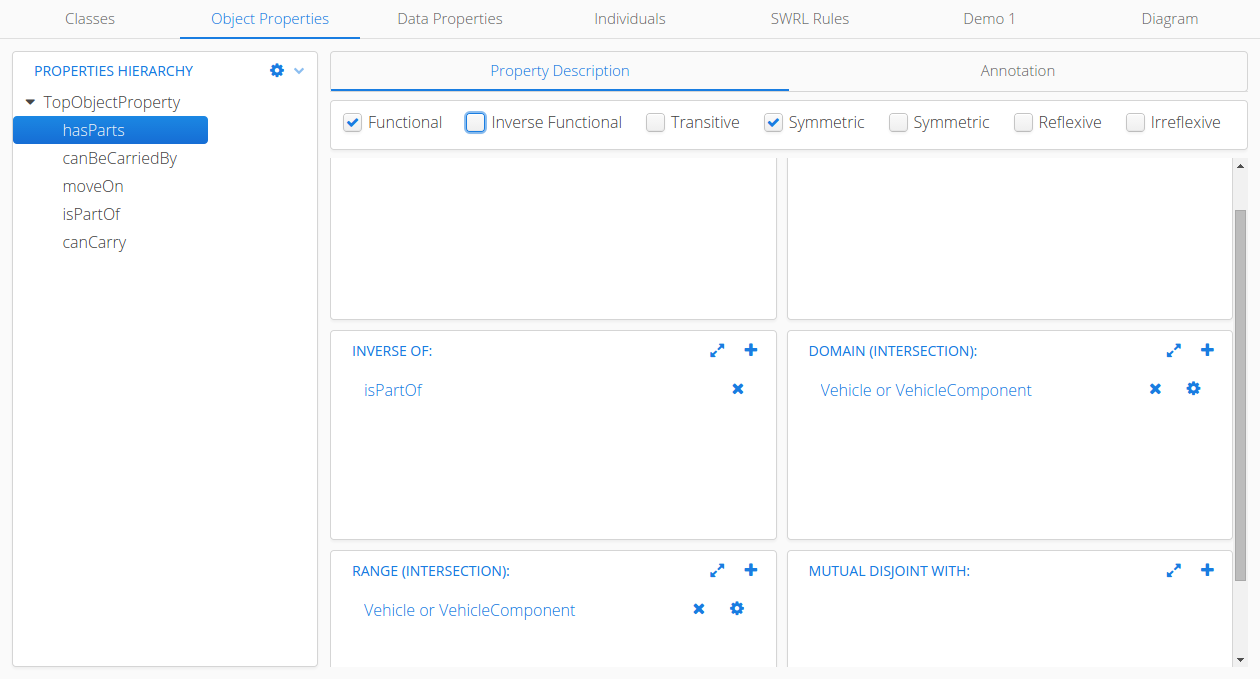
\includegraphics[width=145mm]{Figures/owleditor_opSheet.png}}
	\caption{Object Properties Tab trong UIT-OWL Editor\label{overflow}}
\end{figure}
Tương ứng với lớp \verb|vn.edu.uit.owleditor.view.ObjectPropertiesSheet| trong mã nguồn. Giao diện sử dụng HorizontalLayout của Vaadin gồm 
\begin{enumerate}
\item Panel bên trái là ObjectPropertyHierachicalPanel có một cấu trúc dạng cây với các node đại diện cho các thuộc tính đối tượng trong OWL2 Ontology, với các chức năng thêm/xóa Sibling/Sub Object Property.
\item Một dãy các \textit{CheckBox} dùng để thêm/xóa với các phát biểu trong mục 3.3.6.2 liên quan đến thuộc tính đối tượng được chọn bên trong cấu trúc cây ở bên phải.
\item Các panel nhỏ bên phải được chứa trong lớp ObjectPropertyExpressionPanelContainer, mỗ panel thể hiện một mô tả tương ứng với tên của panel đó về thuộc tính đối tượng đang được chọn trên cấu trúc cây.
\end{enumerate}	

% Data Property Tab
\subsubsection{Tab Data Properties}
\begin{figure}[h!]
	\centering
	\frame{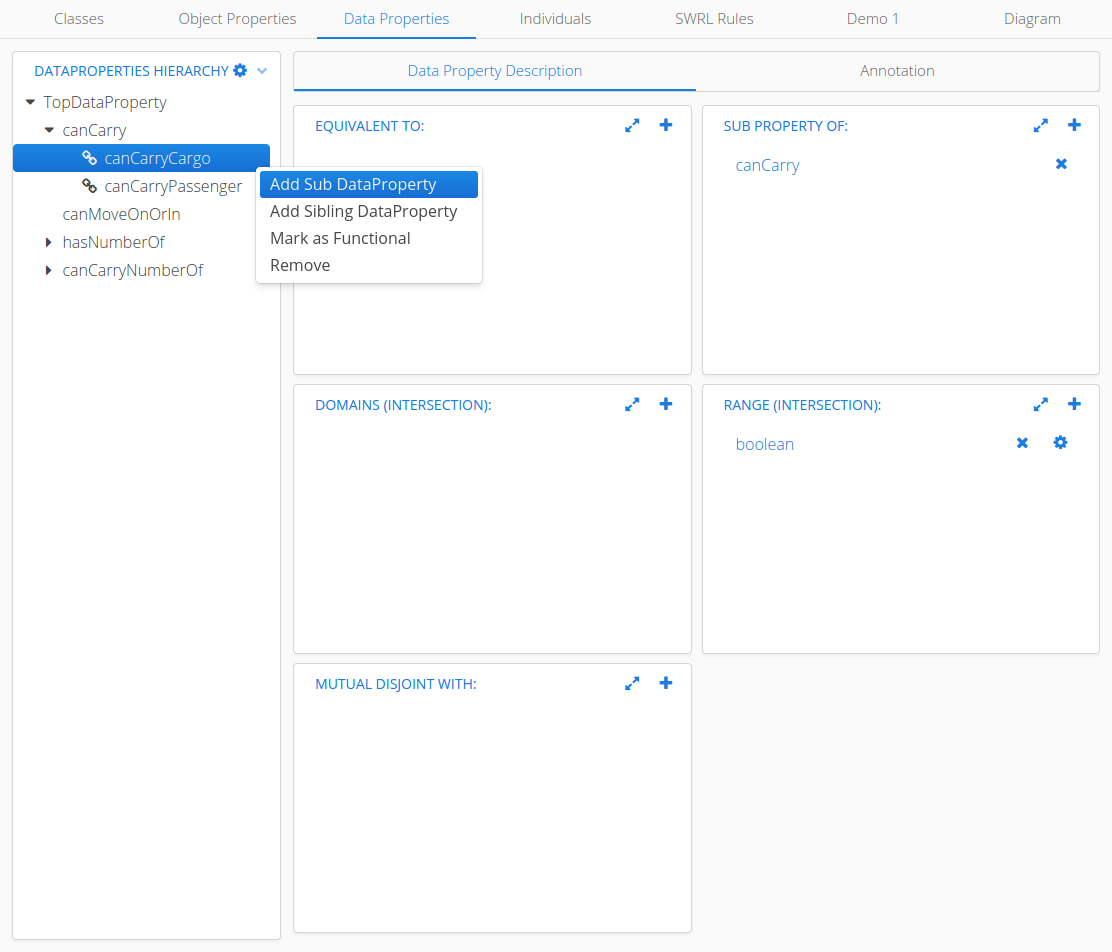
\includegraphics[width=145mm]{Figures/owleditor_dpSheet.png}}
	\caption{Data Properties Tab trong UIT-OWL Editor\label{overflow}}
\end{figure}
Tương ứng với lớp \verb|vn.edu.uit.owleditor.view.DataPropertiesSheet| trong mã nguồn. Các thành phần của tab này gồm:
\begin{enumerate}
\item Panel bên phải là DataPropertyHierachicalPanel có một cấu trúc dạng cây với các node đại diện cho các thuộc tính dữ liệu trong OWL2 Ontology, ngoài chức năng thêm/xóa Sibling/Sub DataProperty còn có tính năng thêm/xóa phát biểu FunctionalDataProperty (những thuộc tính nào có icon phía có nghĩa là có phát biểu FunctionalDataProperty về thuộc tính đó trong ontology.
\item Các panel nhỏ bên phải được chứa trong lớp ObjectPropertyExpressionPanelContainer, mỗ panel thể hiện một mô tả tương ứng với tên của panel đó về thuộc tính dữ liệu đang được chọn bên cấu trúc cây.
\end{enumerate}	

% Individual Tab
\subsubsection{Tab Individual}
\begin{figure}[h!]
	\centering
	\frame{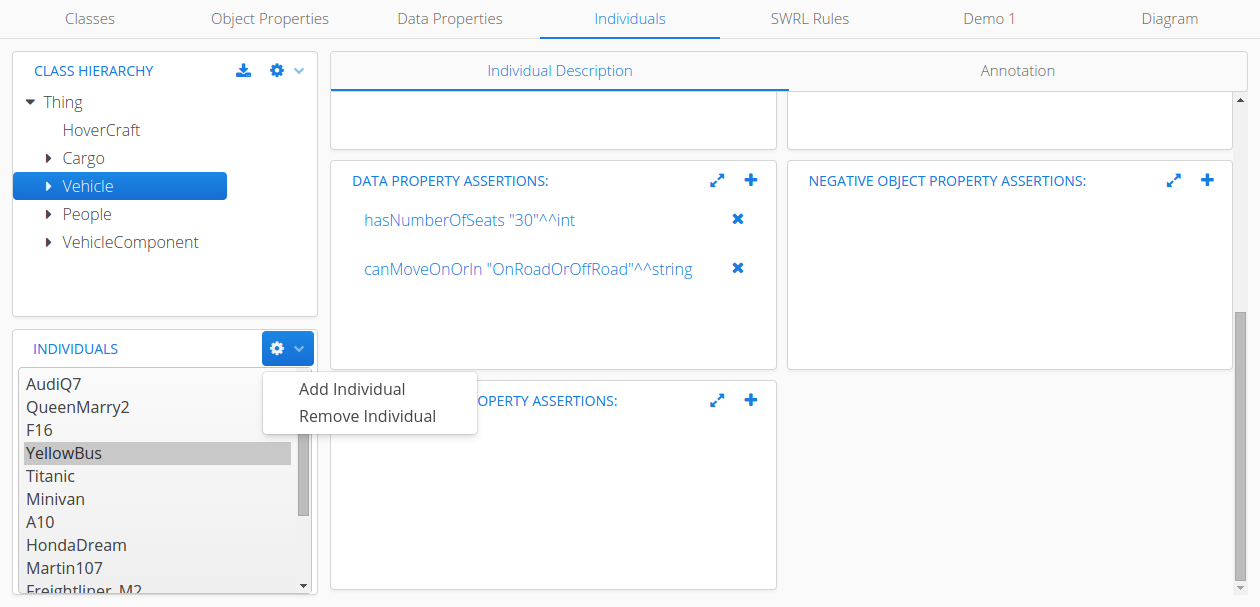
\includegraphics[width=145mm]{Figures/owleditor_individualSheet.png}}
	\caption{Individuals Tab trong UIT-OWL Editor\label{overflow}}
\end{figure}
Tương ứng với lớp \verb|vn.edu.uit.owleditor.view.IndividualsSheet| trong mã nguồn. Các thành phần của tab này gồm:
\begin{enumerate}
	\item Panel bên trái phía trên là ClassHierachicalPanel có một cấu trúc dạng cây với các node chính là các lớp nằm trong OWL2 Ontology, với các chức năng thêm/xóa Sub/Sibling Class. Khi chọn một lớp ở đây thì ListSelect ở bên dưới sẽ hiển thị một danh sách cá thể thuộc lớp này.
	\item Panel bên trái phía dưới là IndividualList hiển thị một danh sách gồm các cá thể thuộc lớp được chọn ở trên, có các tính năng thêm/xóa cá thể.
	\item Các panel bên phải là những panel biểu diễn các phát biểu assertion về cá thể. Tên panel cũng tương ứng với tên phát biểu trong OWL2.
\end{enumerate}

% SWRL Tab
\subsubsection{Tab SWRL}
\begin{figure}[h!]
	\centering
	\frame{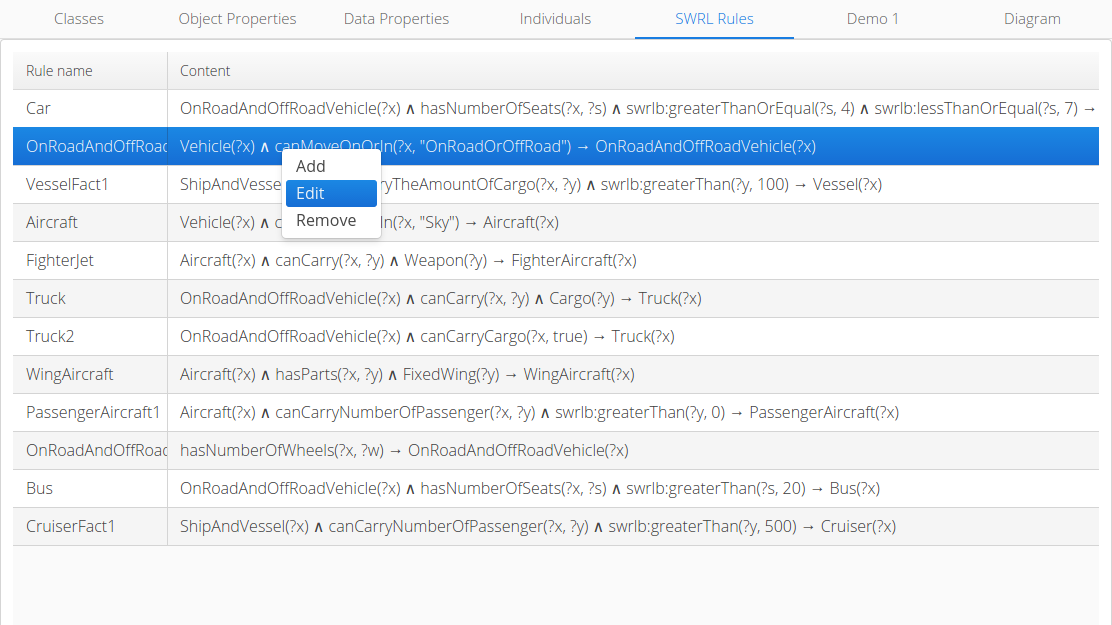
\includegraphics[width=145mm]{Figures/owleditor_swrlSheet.png}}
	\caption{SWRL Rule Tab trong UIT-OWL Editor\label{overflow}}
\end{figure}
Tương ứng với lớp \verb|vn.edu.uit.owleditor.view.RuleSheet| trong mã nguồn. Tab này chỉ gồm một thành phần chính là một Table chứa các SWRL trong tài liệu OWL 2 Ontology. Khi right-click sẽ có các chức năng thêm/xóa/sửa rule được chọn.

\subsubsection{Tab Diagram}
\begin{figure}[h!]
	\centering
	\frame{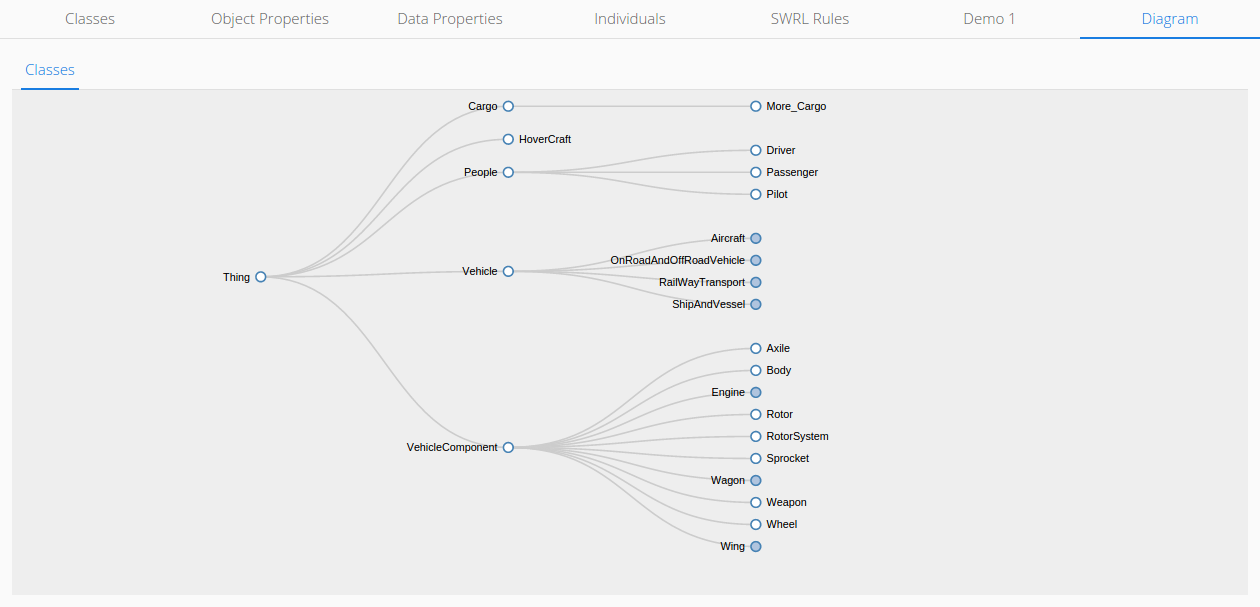
\includegraphics[width=145mm]{Figures/owleditor_diagramSheet.png}}
	\caption{Diagram Tab trong UIT-OWL Editor\label{overflow}}
\end{figure}
Diagram Tab gồm các đồ thị, sơ đồ về biểu diễn cấu trúc phân cáp của lớp bằng các đồ thị từ thư viện D3js.

% Demo Sheet
\subsubsection{Tab Demo}
\begin{figure}[h!]
	\centering
	\frame{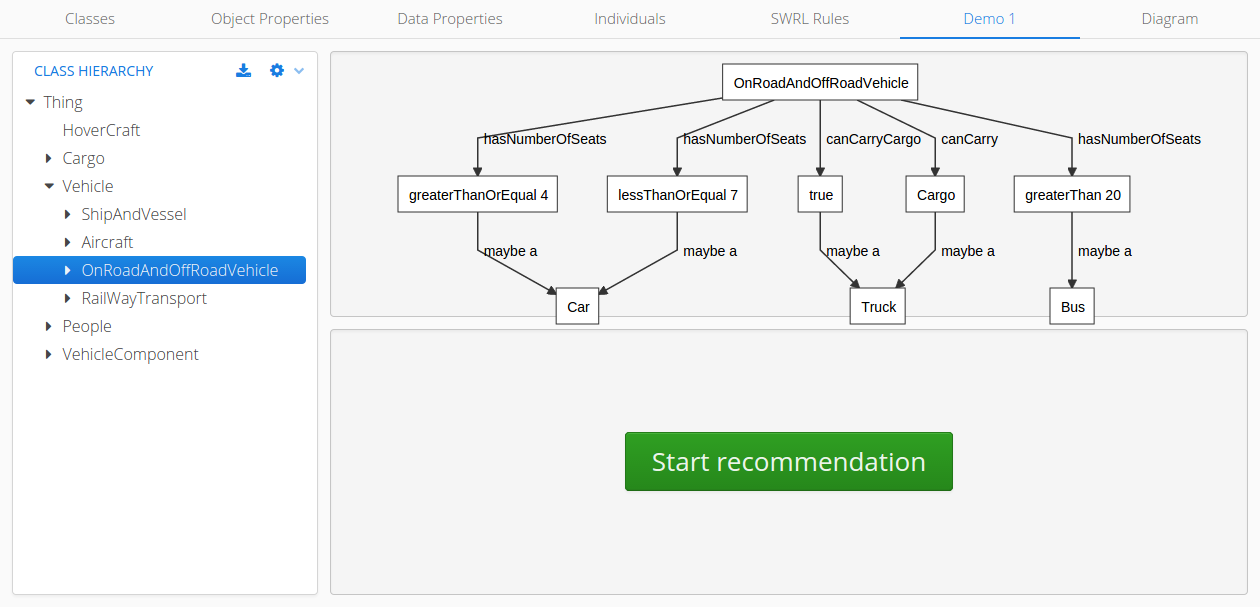
\includegraphics[width=145mm]{Figures/owleditor_demoSheet.png}}
	\caption{Demo Tab trong UIT-OWL Editor\label{overflow}}
\end{figure}
Demo Tab không nằm trong thành phần tiêu chuẩn mà một Ontology Editor bắt buộc phải có như các Tab đã giới thiệu. Tuy nhiên, chúng em cài đặt Demo Tab ở đây với mục đích thử nghiệm tính năng hỗ trợ phân loại (sẽ được đề cập trong phần sau của chương này). Các thành phần của tab này gồm:
\begin{enumerate}
\item Panel bên trái phía trên là ClassHierachicalPanel có một cấu trúc dạng cây với các node chính là các lớp nằm trong OWL2 Ontology, với các chức năng thêm/xóa Sub/Sibling Class. Khi chọn một lớp ở đây thì ListSelect ở bên dưới sẽ hiển thị một danh sách cá thể thuộc lớp này.
\item Panel bên trái phía dưới là IndividualList hiển thị một danh sách gồm các cá thể thuộc lớp được chọn ở trên, có các tính năng thêm/xóa cá thể.
\item Panel phía trên bên phải sẽ hiện thị một sơ đồ thể hiện gợi ý phân loại lớp mà cá thể được chọn đang là thành viên.
\item Panel bên phải phía dưới dùng để điền thêm vào các phát biểu cho cá thể dự theo sơ đồ ở trên.
\end{enumerate}}
% Demo Sheet


\section{OWLEditorKit}
\begin{description}
\item[Interface:] \verb|vn.edu.uit.owleditor.OWLEditorKit|
\item[Class implementation:] \verb|vn.edu.uit.owleditor.OWLEditorKitImpl|
\end{description}
Đây là thành quan trọng nhất của toàn bộ ứng dụng đảm nhiệm việc khai thác các API từ OWL-API, nạp/tạo Ontology từ IRI, suy luận, giải thích các phát biểu, parse các chuỗi viết theo cú pháp \textit{Manchester} thành các mô tả lớp và dữ liệu. Thực ra, các chứng năng vừa kể trên hầu hết đều được thực thi nhờ các API của OWL-API, \textit{OWLEditorKit} đóng gói tất cả lại thành một đối tượng để dễ dàng sử dụng trong các UI Component hơn, cũng như tránh việc phải khởi tạo nhiều lần các API.
\subsection{Các chức năng của OWLEditorKit}

\subsubsection{Load Ontology}
Tương ứng với hàm \textit{loadOntologyFromOntologyDocument}, load các tài liệu OWL2 từ tham số là đối tượng \textit{IRI} của OWL-API, ontology khi load xong sẽ được gán cho đối tượng Active Ontology (sẽ được đề cập ngay sau).
\begin{verbatim}
OWLEditor kit = new OWLEditorKitImpl();
kit.loadOntologyFromOntologyDocument(IRI.create("some url"));
\end{verbatim}
\subsubsection{Giải thích các phát biểu trong OWL2 Ontology}
Tương ứng với hàm \textit{explain}, tham số nhận vào là một phát biểu tương đương đối tượng \textit{OWLAxiom} trong OWL-API. Kết quả trả về là một đối tượng \textit{ExplanationTree} chứa các phát biểu giải thích.

\subsubsection{Xóa các thực thể (Entities) trong OWL2 Ontology}
Xóa các phát biểu trong OWL 2 Ontology không phải là một tác vụ dễ dàng vì một phát biểu có thể được sử dụng để xây dựng nên phát biểu khác. Ví dụ:
\begin{verbatim}
Declaration( Class( A ))
SubClassOf(A B)
EquivalentClasses(A C D)
\end{verbatim}
Giả sử chúng ta muốn xóa phát biểu \textit{Declaration( Class( A ))} thì \textbf{bắt buộc} chúng ta phải xóa luôn những phát biểu có liên quan đến A là \textit{SubClassOf và EquivalentClasses}  bởi vì không có phát biểu khẳng định sự tồn tại của A thì những phát biểu còn lại sẽ trở nên vô nghĩa. Tuy nhiên để thực hiện tác vụ này OWL-API cung cấp cho chúng ta một đối tượng là \textit{OWLEntityRemover} với tính năng duyệt qua mọi phát biểu có liên quan đến thực thể cần xóa, xóa tất cả các phát biểu đó trước khi xóa thực thể. Đối tượng này được sử dụng qua getter \textit{getEntityRemover}.

\subsubsection{Nhà máy sản xuất ra mọi loại đối tượng trong OWL 2 Ontology}
Một chức năng thực sự hữu ích được khai thác từ đối tượng \textit{OWLDataFactory} của OWL-API, với số lượng đối tượng (thực thể, mô tả lớp, thuộc tính, phát biểu, ...) rất lớn để cập ở chương 2, rất khó để chúng ta có thể nhớ và sử dụng chúng dễ dàng. \textit{OWLDataFactory} cung cơ chế để tạo ra mọi loại phát biểu trong OWL 2 Ontology một cách tiện lợi ví dụ như:
\begin{verbatim}
// Declaration( Class(a:Person) )
OWLClass person = factory.getOWLClass("a:Person");

// Declaration( NamedIndividual(a:Peter) )
OWLNamedIndividual Peter = factory.getOWLNameIndividual("a:Peter");

// Declaration( DataProperty(a:HasAge) )
OWLDataProperty hasAge = factory.getOWLDataProperty("a:HasAge");

// ClassAssertion( a:Person a:Peter )
OWLClassAssertionAxiom axiom1 = 
         factory.getOWLClassAssertionAxiom(person, Peter);
         
// "22"^^xsd:integer 
OWLLiteral age = factory.getOWLLiteral(22);

// DataPropertyAssertion( a:HasAge a:Peter "22"^^xsd:integer); 
OWLDataPropertyAssertionAxiom phatbieu = 
         factory.getOWLDataPropertyAssertionAxiom(hasAge, Peter, age);
\end{verbatim}
Trong \textit{OWLEditorKit}, \textit{OWLDataFactory} được truy xuất qua getter \textit{getOWLDataFactory()}.

\subsubsection{Nhà máy sản xuất ra mọi loại đối tượng dữ liệu cho ứng dụng UIT-OWL Editor}
{\let\thefootnote\relax\footnotetext{
		*: \textit{http://en.wikipedia.org/wiki/Factory\_method\_pattern}}
}
\begin{description}
\item[Interface:] \verb|vn.edu.uit.owleditor.data.OWLEditorDataFactory|
\item[Class Implementation:] \verb|vn.edu.uit.owleditor.data.OWLEditorDataFactoryImpl|
\end{description}
Học tập mô hình \textit{Factory Pattern} \textsuperscript{*} từ đối tượng \textit{OWLDataFactory}, chúng em cũng tự xây dựng một đối tượng với mục tiêu là cung cấp một cơ chế tiện lợi để tạo ra các đối tượng dữ liệu và các event trong UIT-OWL Editor. Tham số khởi tạo của \textit{OWLEditorDataFactory} chính là \textit{OWLEditorKit}. Ví dụ để tạo sự kiện thêm một phát biểu về lớp vào Ontology:
\begin{verbatim}
// Khởi tạo OWLEditorDataFactory
OWLEditorKit kit = new OWLEditorKit();
OWLEditorDataFactory editorFactory = new OWLEditorDataFactoryImpl(kit);
// Tạo sự kiện thêm phát biểu về lớp
OWLClass person = factory.getOWLClass("a:Person");
OWLClass man = factory.getOWLClass("a:Man");
OWLEditorEvent.ClassAxiomAdded event =
        owlEditorDataFactory.getSubClassOfAddEvent(man, person);
\end{verbatim}
Một cái nhìn chi tiết vào trong \textit{OWLEditorDataFactoryImpl} sẽ làm gì với dòng cuối cùng trong đoạn code ở 
\begin{verbatim}
// Bên trong lớp OWLEditorDataFactoryImpl
private final OWLEditorKit editorKit;
public OWLEditorDataFactoryImpl(OWLEditorKit eKit) {
   this.editorKit = eKit;
}
...
OWLEditorEvent.ClassAxiomAdded getClassAssertionAddEvent(OWLClass owner,
  OWLNamedIndividual expression) {

  return new OWLEditorEvent.ClassAxiomAdded(editorKit.getOWLDataFactory()
                    .getOWLClassAssertionAxiom(owner, expression), owner);
}
\end{verbatim}
Để sử dụng đối tượng \textit{OWLEditorDataFactory}, chúng ta sẽ sử dụng qua getter \textit{OWLEditorDataFactory} của \textit{OWLEditorKit} để tránh khởi tạo nhiều lần (đối tượng này đã được khởi tạo ngay bên trong \textit{OWLEditorKitImpl}.

\subsubsection{Parse chuỗi thành các mô tả lớp (OWLClassExpression)}
OWLEditorKit cũng được tích hợp một đối tượng \textit{ManchesterOWLSyntaxParser} trong OWL-API, nhiệm vụ là để parse các đoạn text từ người dùng theo cú pháp \textit{Manchester} thành các mô tả lớp (OWLClassExpression) hay các miền dữ liệu (OWLDataRange). Parser này được sử dụng thông qua getter \textit{getParser} hoặc parse trực tiếp qua hàm \textit{parseClassExpression(String stringToParse)} . Ví dụ:
\begin{verbatim}
OWLEditorKit eKit = new OWLEditorKitImpl();
// nạp ontology ...
// Cách 1
ManchesterOWLSyntaxParser parser = eKit.getParser();
parser.setStringToParse("Has some Friend");
OWLClassExpression ce1 = parser.parseClassExpression();
// Cách 2 
OWLClassExpression ce2 = eKit.parseClassExpression("Has some Kid");
\end{verbatim}

\subsubsection{Suy luận các phát biểu}
Tính năng suy luận được đáp ứng bới Pellet Reasoner đề cập ở chương trước. Reasoner cũng đã được tạo sẵn trong \textit{OWLEditorKitImpl}, truy cập thông qua getter \textit{getReasoner()} và sử dụng như mô tả ở chương trước.

\subsubsection{Áp dụng các thay đổi về phát biểu cho ontology}
Chức năng này được thực thi bởi đối tượng \textit{OWLOntologyManager} được khởi tạo cùng với lớp \textit{OWLEditorKitImpl}, sử dụng thông qua getter \textit{getModelManager()}.
\textit{OWLOntologyManager} sẽ được sử dụng để áp dụng thay đổi trong các hàm Subscriber (sẽ được đề cập trong phần Xử lý sự kiện).

\subsection{Một số đối tượng đáng chú ý khác trong OWLEditorKitImpl}
Ngoài các chức năng đi kèm với các đối tượng quan trong kể trên trong implementation của \textit{OWLEditorKit} cũng có một số đối tượng mà chúng ta cũng cần phải lưu ý.
\subsubsection{Active Ontology}
Biến  \textit{activeOntology} là một đối tượng \textit{OWLOntology} của OWL-API được khai báo trong \textit{OWLEditorKitImpl}. Biến này chính là OWL2 Ontology hiện hành đang được thao tác trên giao diện. Các thao tác thêm/xóa/sửa các phát biểu qua các giao diện đều sẽ được cập nhật và áp dụng lên đối tượng \textit{OWLOntology} này.
\subsubsection{Manchester Renderer}
Hàm static \textit{OWLEditorKitImpl.render(OWLObject)} dùng render hay chuyển đổi các đối tượng OWL 2 thành dạng chuỗi (cú pháp Manchester), chủ yếu để render các phát biểu, mô tả lớp/thuộc tính/kiểu dữ liệu.
\subsubsection{Lấy tên thực thể}
Hàm static \textit{OWLEditorKitImpl.getShortForm(OWLEntity)} dùng lấy tên các đối tượng \textit{OWLEntity}. Ví dụ: \textit{longIRI:Person} -> \textit{Person}


\section{Xử lý sự kiện trong UIT-OWL Editor}
{\let\thefootnote\relax\footnotetext{
		*: \textit{http://en.wikipedia.org/wiki/Publish\%E2\%80\%93subscribe\_pattern}}
}
Để xử lý các sự kiện trong ứng dụng, chúng em sử dụng thư viện Guava EventBus \cite{guava}. \textit{EventBus} cho phép giao tiếp theo kiểu công bố và theo dõi (\textit{publish-subscribe}\textsuperscript{*}), các UI Component không cần thiết phải khai báo với nhau (để biết được tồn tại của nhau). Thư viện được được thiết kế nhằm thay thế kiểu giao tiếp chia sẻ sự kiện trong tiến trình (in-process event distribution) bằng cách khai báo rõ ràng các thành phần có liên quan tới sự kiện với nhau (khai báo đối tượng tạo ra sự kiện, đối tượng sẽ lắng nghe sự kiện với nhau). Cơ chế xử lý sự kiện này của ứng dụng có thể được miêu tả trong hình sau:
\begin{figure}[h!]
	\centering
	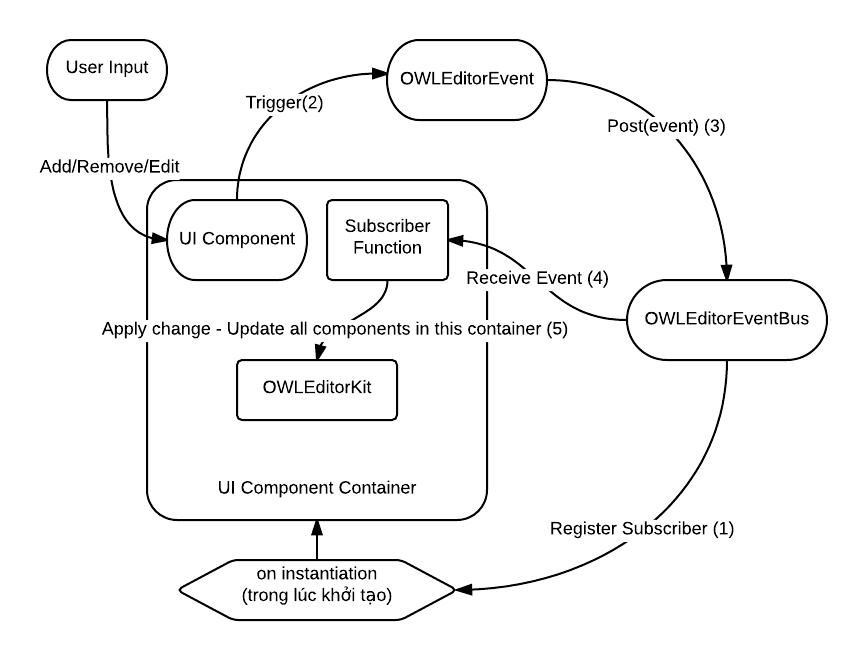
\includegraphics[width=145mm]{Figures/owleditor_eventBus.png}
	\caption{Xử lý sự kiện trong UIT-OWL Editor\label{overflow}}
\end{figure}
Để hiểu rõ hơn nữa, chúng em xin được lấy sự kiện thêm một phát biểu \textit{SubClassOf} trong Panel có tên tương ứng nằm trong Tab "Classes". Panel này là một đối tượng lớp \textit{ClassPanel} nằm trong \textit{ClassExpressionPanelContainer} và các chức năng \textit{EventBus} của toàn ứng dụng có thể được sử dụng qua lớp \textit{OWLEditorEventBus}. 
\begin{verbatim}
class ClassExpressionPanelContainer extends AbstractPanelContainer {
    ClassPanel subClsPanel; 
    public ClassExpressionPanelContainer {
       subClsPanel = new ClassPanel("SubClass Of: ") {
          void initActionADD() { 
          // Mở một cửa số nhỏ nhằm nhập mô tả lớp mới vào
          UI.getCurrent()
            .addWindow(new buildAddClassExpressionWindow(...));            
             ...
          }
       }
       this.addComponent(subClsPanel); 
	   OWLEditorEventBus.register(this); // Bước 1 trong sơ đồ
    }
    ...
    // Annotation @Subscribe được cung cấp bởi thư viện EventBus
    // Bước 4 trong sơ đồ 
    @Subscribe 
    public void handlAxiomAdd(OWLEditorEvent.ClassAxiomAdded event) {
       // Bước 5 trong sơ đồ
       OWLEditorKit kit = OWLEditorUI.getEditorKit();
       kit.getModelManager.applyChange(new 
           AddAxiom(kit.getActiveOntology(),event.getAxiom));
	       // render các thay đổi lên các UI Components
    }  
}
class buildAddClassExpressionWindow extends ... {
    ...
    // sự kiện khi nhấn save tương ứng bước 2 trong sơ đồ
    Button.ClickListener initSaveListener() {
       return click -> {
          OWLClassExpression ce = editorKit
            .parseClassExpression("some value from Textfield");
          // tương ướng bước 3 
          OWLEditorEventBus.post(ClassAxiomAdded(.., ce));
       }
    }
}
\end{verbatim}
Hình sau miêu tả lại thao tác người dùng trên UI:
\begin{figure}[h!]
	\centering
	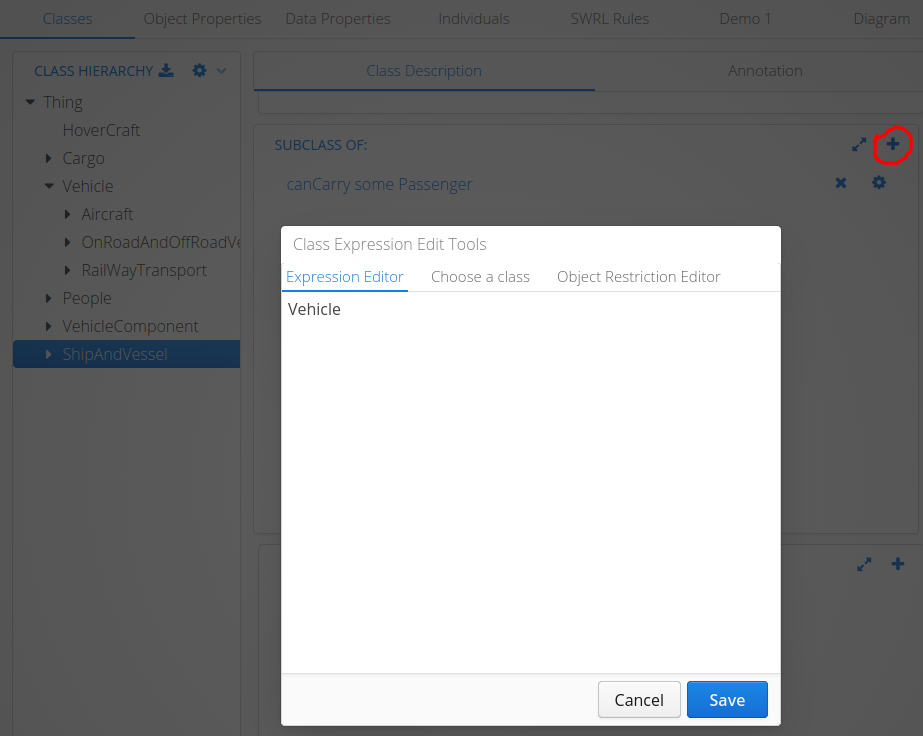
\includegraphics[width=145mm]{Figures/eventBusExplain.png}
	\caption{Xử lý sự kiện trong UIT-OWL Editor\label{overflow}}
\end{figure}
Đầu tiên trước khai mọi sự kiện diễn ra một \textit{Subscriber} cần được đăng ký trong một Component nào đó bằng Annotation @Subscribe và method \textit{register} (đăng ký đây sẽ là listener/subscriber để theo dõi các sự kiện tương ứng). Khi người dùng, nhấn dấu cộng ở góc của Panel \textit{SubClassOf} sẽ mở ra một cửa sổ để nhập vào mô tả lớp, nút save được bấm thì cũng là lúc mà sự kiện được công bô (publish) lên \textit{EventBus} (qua phương thức \textit{post} ở bước 3), do đã đăng ký trước nên phương thức \textit{Subscribe} sẽ được EventBus truyền cho đúng kiểu event mà nó đang theo dõi. Lưu ý: là phương thức nào làm Subscriber thì bắt buộc phải có một tham số duy nhất là sự kiện với kiểu tương ứng với nơi mà sự kiện đó được công bố, đồng thời access-level của phương thức phải là public.
\\
Như đã nếu, nguyên tắc của EventBus để phân biệt các sự kiện chỉ là kiểu của nó. Chính vì thế mà với mỗi loại hành động thêm/xóa/sửa trên loại thực thể, hoặc phát biểu của thực thể sẽ có một loại sự kiện tương ứng. Ví dụ: đối với các phát biểu liên quan tới lớp sẽ có 3 loại tương ứng là ClassAxiomAdded, ClassAxiomRemoved và ClassAxiomEdit. Tương tự cho các thực thể và phát biểu còn lại. Chi tiết hơn, thầy cô và bạn đọc có thể tham khảo thêm trong lớp \textit{vn.edu.uit.owleditor.event.OWLEdtiorEvent} trong mã nguồn của ứng dụng \cite{owleditorSrc}.


\section{Tổ chức các đối tượng dữ liệu - Data Model}
Đã được đề cập trong lúc giới thiệu về Vaadin, data model trong Vaadin được chia làm 3 cấp từ thấp đến cao Property, Item và Container. Trong ứng dụng, chúng em chỉ sử dụng 2 dạng data model là Property và Container. 
\subsection{HierarchicalContainer}
%Vaadin cung cấp một lớp gọi là \textit{HierarchicalContainer} chuyên dùng để chứa dạng dữ liệu có cấu trúc phân cấp. Qua giới thiệu ở chương 2, chúng ta đã biết rằng các t đều là những đối tượng có quan hệ SubClassOf, SubObjectPropertyOf và SubDataPropertyOf hay có thể nói 3 thực thể kể trên có cấu trúc phân cấp.
Để thể hiện tính chất phân cấp của các thực thể như lớp, thuộc tính đối tượng và dữ liệu trong OWL 2 Ontology, chúng ta có thể dùng Tree Component của Vaadin. Tuy nhiên, với việc UI Component Tree được sử dụng lặp lại nhiều lần trong ứng dụng, nên việc tách biệt các đối tượng dữ liệu với UI đã sẽ giúp chúng ta tiết kiệm được những khai báo lại không cần thiết, dữ liệu thay đổi trong DataModel cũng sẽ được cập nhật đến toàn bộ những UI Component mà nó được sử dụng (binding). Để hiểu rõ hơn về cách tổ chức của \textit{HierarchicalContainer} chúng em xin được lấy  \textit{AbstractOWLObjectHierarchicalContainer}, được thừa kế bởi \textit{HierarchicalContainer} của lớp, thuộc tính đối tượng và dữ liệu. Nó gồm những đặc điểm quan trọng sau:
\begin{itemize}
\item Thừa kế từ HierarachicalContainer của Vaadin nên sẽ có sẵn các phương thức \textit{addItem}, \textit{setParent} phục vụ cho việc thêm, và sắp xếp item theo cấu trúc cây.
\item Gồm một \textit{OWLEntityRemover} dùng để xóa thực thể (OWLEntity) khi nhận yêu cầu xóa từ UI Component.
\item Gốm một đối tượng OWLNamedObjectVisitor (xem lại Visitor Pattern ở chương trước) có chức năng tìm đóng loại cá thể, sau đó thêm chúng vào HierachicalContainer.
\item Gồm một \textit{OWLOntologyChangeVisitor} dùng để cập nhật sự thay đổi trong container cho đồng bộ với sự thay đổi của OWLOntology khi thêm/xóa các thực thể và phát biểu SubClass/SubPropertyOf.
\item Gồm một hàm đệ quy với mục đích là sắp xếp các item trong HierarchicalContainer cho đúng với sự phân cấp của chúng trong OWL2 Ontology.
\end{itemize}
Dưới đây là sơ đồ mô tả lại giải thuật thêm và sắp xếp các item lên cấu trúc cây của \textit{OWLClassHierarchicalContainer} thừa kế từ lớp Abstract ở trên. Chú thích: \textit{contains} là một hàm nhằm xác định đối tượng được xét đã tồn tại trong Container chưa.
\begin{figure}[h!]
	\centering
	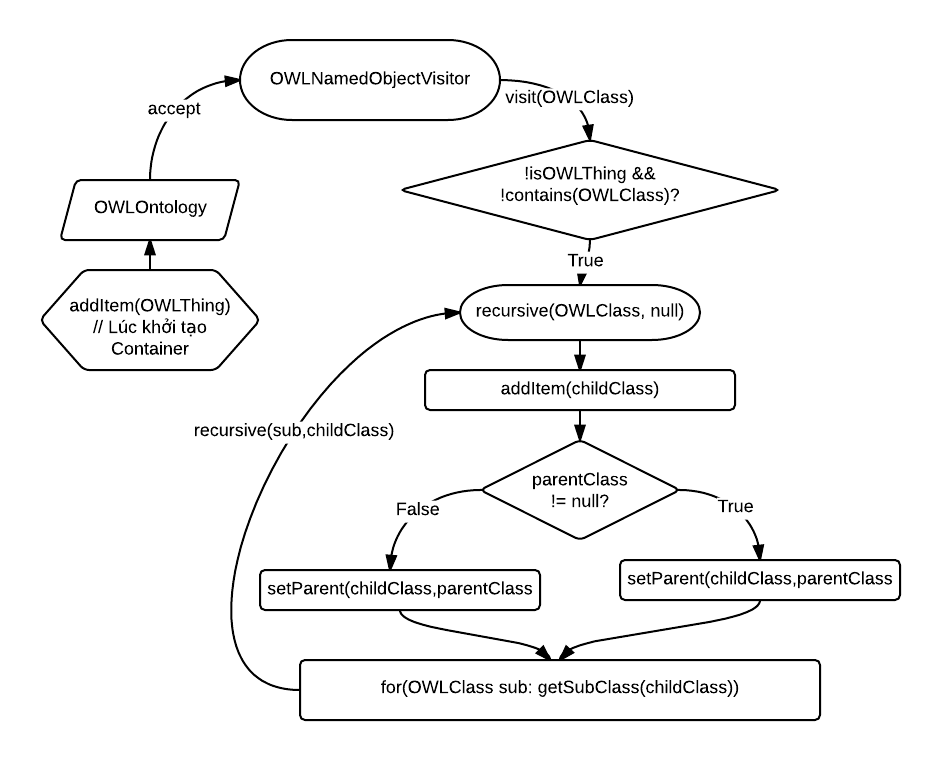
\includegraphics[width=150mm]{Figures/owleditor_hccontainer.png}
	\caption{OWLClassHierarchicalContainer trong UIT-OWL Editor\label{overflow}}
\end{figure}
\subsection{List}
Đây thật ra là lớp mà HierarchicalContainer trong Vaadin thừa kế IndexedContainer, mục đích của Container dạng này là dùng để chứa các item theo dạng danh sách, chúng em sử dụng chúng để chứa các đối tượng như OWLNamedIndividual, OWL2Datatype . Bảng sau liệt kê đối tượng của các Container dạng này trong ứng dụng.
\begin{table}[h!]
	\centering
	\begin{tabular}{|l|l|}
		\hline
		IndexContainer  & Đối tượng chứa \\
		\hline
		DataRangeShortFormContainer	& OWLDatatype dạng ShortForm(String) \\ 
		\hline
		OWL2DatatypeContainer	& OWLDatatype  \\
		\hline
		OWLEntitiesShortFormContainer & OWLEntity dạng ShortForm(String)	\\	
		\hline
		OWLNamedIndividualContainer & OWLNamedIndividual  \\		
		\hline
	\end{tabular}
	\caption{List Container trong UIT-OWLEditor\label{overflow}}
\end{table}
\subsection{Property}
Mục đích đưa các đối tượng thành Property của Vaadin cũng tương tự như Container, các đối tượng OWL2 sẽ được sử dụng lại nhiều lần bởi các UI Component sử dụng (binding) nó nên sử dụng Property chứa các đối tượng OWLObject sẽ giúp tiết kiệm những lần truyền tham số (là các OWLObject) giữa các UI Component. Các Property và đối tượng OWLObject tương ứng được tổng hợp trong bảng sau.
\begin{table}[H]
	\centering
	\begin{tabular}{|l|l|}
		\hline
		Property & OWLObject tương ứng  \\
		\hline
		OWLClassSource	& OWLClass \\ 
		\hline
		OWLDataPropertyExpressionSource & OWLDataPropertyExpression  \\
		\hline
		OWLObjectPropertySource & OWLObjectProperty  \\		
		\hline
		OWLDataPropertySource	& OWLDataProperty   \\
		\hline
		OWLNamedIndividualSource& OWLNamedIndividual   \\
		\hline
		OWLDataRangeSource	& OWLDataRange   \\
		\hline
		OWLPropertySource 	& OWLProperty   \\
		\hline
		OWLLogicalEntitySource & OWLLogicalEntity \\
		\hline
		OWLEntitySource	& OWLEntity	 \\
		\hline
		OWLLiteralSource	& OWLLiteral \\
		\hline
		OWLPropertyAssertionObjectSource & OWLPropertyAssertionObject \\
		\hline
		OWLClassExpressionSource	& OWLClassExpression \\		
		\hline
		OWLPropertyExpressionSource	& OWLPropertyExpression  \\		
		\hline
		OWLDataPropertyExpressionSource	& OWLDataPropertyExpression \\		
		\hline
		OWLObjectPropertyExpressionSource	& OWLObjectPropertyExpression \\
		\hline	
		SWRLRuleSource	& SWRLRule	 \\
		\hline
		SWRLAPIRuleSource	& SWRLAPIRule \\
		\hline
		OWLObjectSource & OWLObject \\
		\hline
	\end{tabular}
	\caption{Các Property trong UIT-OWL Editor\label{overflow}}
\end{table}
\subsection{Converter}
Trong ứng dụng chúng em có sử dụng một số Converter tự định nghĩa vốn được xây dựng từ interface Converter (phần giới thiệu Vaadin Framework) với mục đích chuyển đổi các thực thể gồm lớp, thuộc tính đối tượng, thuộc tính dữ liệu và cá thể có tên. Mục tiêu xây dựng các Converter này là sẽ giúp chuyển đối giữ chuỗi sang đối tượng tương ứng là OWLClass, OWLObjectProperty, OWLDataProperty và OWLNamedIndividual một cách nhanh chóng khi thêm các cá thể mới. Ví dụ:
\begin{figure}[h!]
	\centering
	\frame{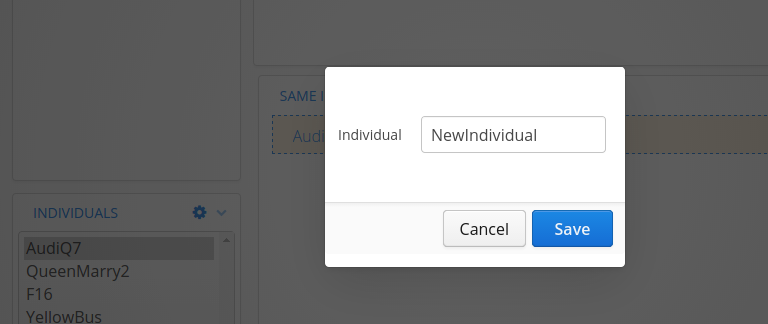
\includegraphics[width=140mm]{Figures/owleditor_converter.png}}
	\caption{Converter trong UIT-OWL Editor\label{overflow}}
\end{figure}
TextField mà trong hình được cài đặt converter:
\begin{verbatim}
textField.setConverter(new StringToNamedIndividualConverter(editorKit));
// Bên trong StringToNamedIndividualConverter 
// Hàm đổi chuỗi thành OWLNamedIndividual
public OWLNamedIndividual convertToModel(String valueInTextField,
                          Class<? extends OWLNamedIndividual> targetType,
                          ...) {
   ...
   return editorKit.getOWLDataFactory()
                   .getOWLNamedIndividual(valueInTextField,
                                  editorKit.getPrefixManager());
}                          
\end{verbatim}
Các converter còn lại cũng có cơ chế tương tự trong ví dụ này, chi tiết hơn có thể xem package \textit{vn.edu.uit.owleditor.utils.converter} \cite{owleditorSrc}.

\section{Các tính năng nổi bật của UIT-OWL Editor}
Ngoài những tính năng đã trình bày sơ qua trong phần đầu UI, phần này chúng em xin dành để liệt kê ra một số tính năng nổi bật trong ứng dụng.

\subsection{Trình biên tập các mô tả lớp}
Trình biên tập cho phép nhập các chuỗi các khai báo về mô tả lớp (class expression) theo cú pháp Manchester, trình biên tập mô tả lớp cũng được tích hợp một danh sách autocomplete gồm các thực thể đã được khai báo trong ontology. Mỗi loại cá thể trong danh sách autocomplete sẽ được hiện thị theo một Icon khác nhau tương ứng với chữ cái đầu tiên của loại đó như \textbf{O} cho ObjectProperty, \textbf{C} cho Class, \textbf{D} cho DataProperty và \textbf{I} cho NamedIndividual. Khi nhấn nút save, ứng dụng sẽ tự động parse chuỗi thành Đối tượng OWLClassExpression bằng ManchesterSyntaxParser trong OWLEditorKit, sẽ có thông báo lỗi nếu cú pháp nhập sai.
\begin{figure}[h!]
	\centering
	\frame{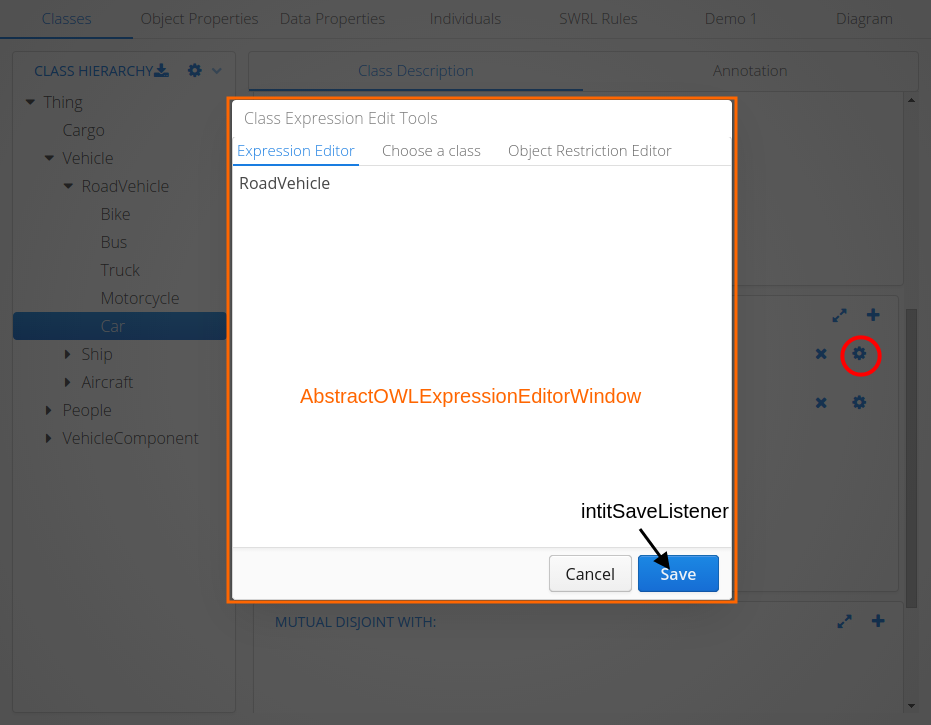
\includegraphics[width=145mm]{Figures/owleditor_ceeditor.png}}
	\caption{Biên tập mô tả lớp trong UIT-OWL Editor\label{overflow}}
\end{figure}
\\
Lý do chọn Manchester Syntax vì chúng em nhận thấy cú pháp của nó thân thiện, gần với ngôn ngữ con người hay sử dụng hàng ngày (thầy cô và bạn đọc có thể xem lại trong chương giới thiệu về OWL 2).
\subsection{Trình biên tập SWRL Rule}
Trình biên tập cho phép biên tập SWRL Rule bằng cú pháp được giới thiệu trong chương \textit{Semantic Web Rule Language}, tổ chức các Rule theo tên, và thêm giải thích cho Rule.
\begin{figure}[h!]
	\centering
	\frame{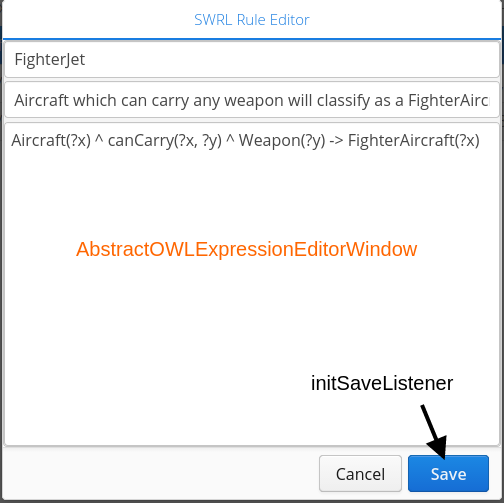
\includegraphics[width=145mm]{Figures/owleditor_ruleeditor.png}}
	\caption{Biên tập SWRL Rule trong UIT-OWL Editor\label{overflow}}
\end{figure}
Trình biện tập rule được đảm nhiệm bởi thành phần \textit{SWRLAPIRuleOntology} trong \textit{OWLEditorKit} đã được giới thiệu ở trên.

\subsection{Tính năng suy luận Reasoning}
Để sử dụng tính năng suy luận, chúng ta chọn biểu tượng bánh răng ở góc phải của Panel chứa cây các lớp trong Ontology, sẽ mở ra một menu với tùy chọn "Start reasoner". Hãy chọn nó, chương trình sẽ thông báo "Reasoner Activated". Đối với Tab \textit{Individual}, chọn bất kì một lớp nào trong cây rồi chọn một trong các cá thể của lớp đó, các phát biểu có liên quan đến cá thể đó sẽ hiển thị các panel nhỏ tương ứng với các loại phát biểu của cá thể.
\begin{figure}[h!]
	\centering
	\frame{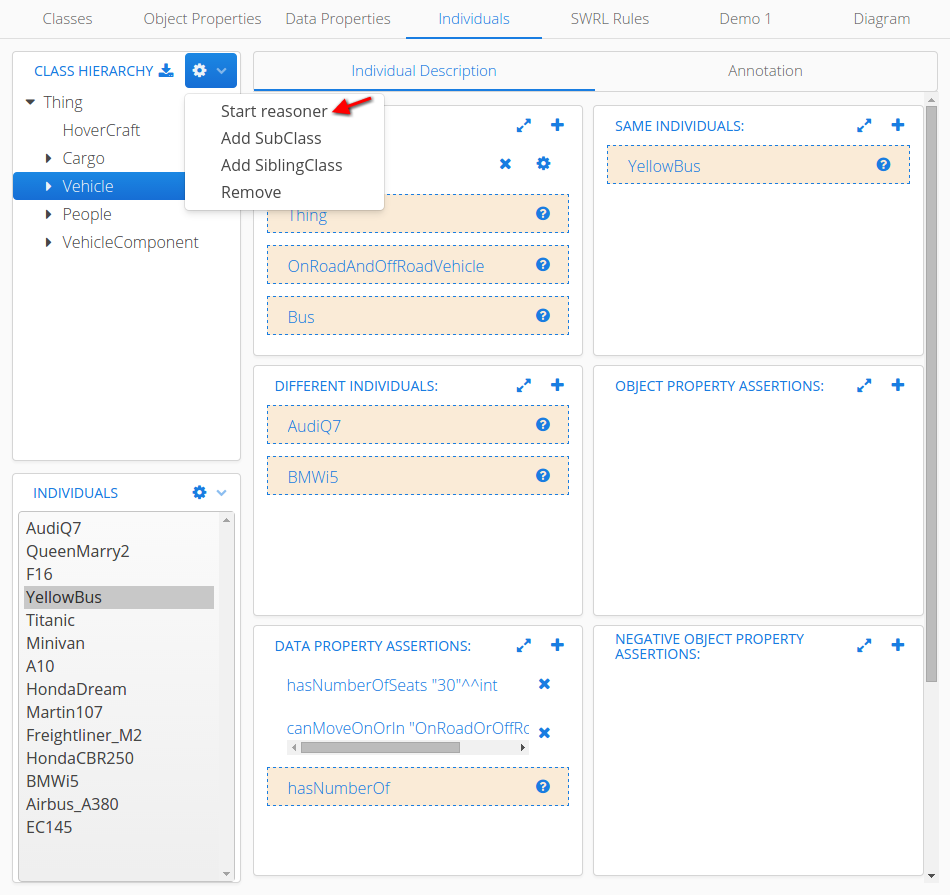
\includegraphics[width=145mm]{Figures/owleditor_reasoning.png}}
	\caption{Tính năng suy luận trong UIT-OWL Editor\label{overflow}}
\end{figure}
Trong hình, các phát biểu được tô đậm chính là các phát biểu được suy luận ra từ Ontology nhờ Pellet Reasoner. Để xem giải thích tại sao cho các phát biểu này chúng ta chọn biểu tượng ? ở cuối mỗi phát biểu. Ví dụ để xem tại sao cá thể \textit{AudiQ7} lại được phân loại thuộc lớp \textit{Car} chúng ta chọn biểu tượng ? ở cuối phát biểu \textit{"Car"}.
\begin{figure}[H]
	\centering
	\frame{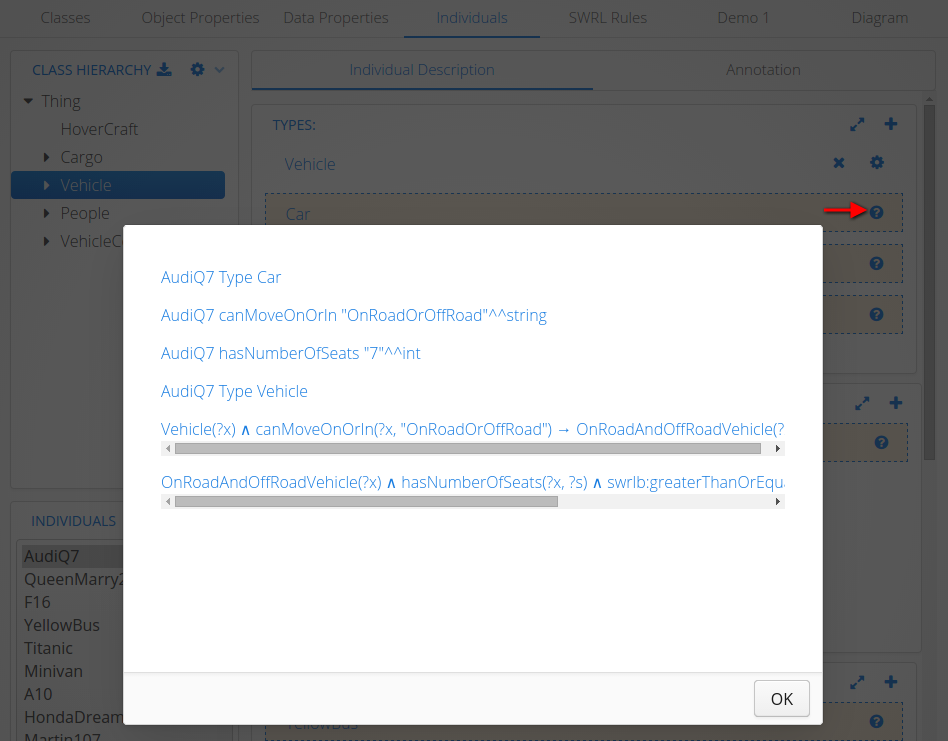
\includegraphics[width=145mm]{Figures/owleditor_explanationWindow.png}}
	\caption{Giải thích suy luận trong UIT-OWL Editor\label{overflow}}
\end{figure}
Việc giải thích được đảm nhiệm bởi đối tượng \textit{DefaultExplanationGenerator} của OWL-API hoạt động theo nguyên lý được mô tả ở chương \textit{"Tính nhất quán của Ontology"}.

\section{Thử nghiệm tính năng hỗ trợ phân loại - Demo Tab}
Bên cạnh việc sử dụng tính năng suy luận mà OWL 2 Ontology cung cấp qua đặc điểm ngôn ngữ của nó hay cộng với sự hỗ trợ từ SWRL Rule











%% end chapters
\clearpage
%% ----------------------------------------------------------------


%% ----------------------------------------------------------------
% Now begin the Appendices, including them as separate files

\addtocontents{toc}{\vspace{2em}} % Add a gap in the Contents, for aesthetics

\appendix % Cue to tell LaTeX that the following 'chapters' are Appendices

\chapter{Giả định thế giới mở vs. Giả định thế giới đóng}
\section{Vậy OWA và CWA được sử dụng khi nào ?}
Giả định thế giới đóng (CWA) được sử dụng khi một hệ thống đã có đầy đủ thông tin. Đây là trường hợp được áp dụng cho nhiều ứng dụng cơ sở dữ liệu. Ví dụ, xem xét một tình huống một ứng dụng cơ sở dữ liệu đặt vé máy bay, chúng ta tìm kiếm đường bay thẳng Phú Quốc và Hà Nội, và kết quả là nó không tồn tại trong cơ sở dữ liệu (không quan tâm đến thực tế có hay không có đường bay này). Và theo CWA nên câu trả lời từ cơ sở dữ liệu là : "Không có đường bay thẳng Hà Nội - Phú Quốc" (Một giả định là thực tế cũng không tồn tại đường bay này do cơ sở dữ liệu không biết). Đây là dạng ứng dụng mà người dùng mong đợi một câu trả lời chính xác ( phổ biến ở các cở sở dữ liệu quan hệ).
\\
Ngược lại với Giả định thế giới đóng, Giả định thế giới mở đươc áp dụng trên một hệ thống mà thông tin được cung cấp không đầy đủ. Đây là trường hợp chúng ta một biểu dạng một dạng tri thức (a.k.a Ontologies) và chúng ta muốn khám phá những thông tin mới tiềm ẩn trong đó. Ví dụ, xem xét một hệ thống lưu trữ tiền sử bệnh lý của bệnh nhân. Nếu cơ sở dữ liệu không chứa thông tin về một dạng dị ứng cụ thể mà bệnh nhân mắc phải, điều đó không đồng nghĩa là bệnh nhân đó không mắc phải nó trên thực tế. Từ đó câu trả lời từ cở sở dữ liệu theo chuẩn OWA sẽ là : "Không rõ bệnh nhân này có mắc phải dị ứng đó không, trừ khi có những thông tin đầy đủ hơn được cung cấp".
\section{So sánh OWA và CWA}
Giả định Thế Giới Đóng không chỉ là trả về các câu trả lời \textit{"không"} và Giả định Thế Giới Mở không chỉ là về trả về \textit{"không biết"}. Lấy lại ví dụ trên: "\textbf{A} là một công dân Hoa Kỳ" và giả sử khẳng định sau là đúng: "Một người chỉ có thể là công dân của một quốc gia". Chúng ta cùng xem tiếp câu sau: "A là công dân Việt Nam". Xét theo Giả định Thế Giới Đóng (CWA), phát biểu này có thể gây ra lỗi, vì nó mâu thuẫn với 2 phát biểu ban đầu giả sử chúng ta biết Mỹ và Việt Nam là 2 quốc gia khác nhau . Nếu đem phát biểu vừa rồi xét trong Giả định thế giới mở, thay vì gây lỗi, nó sẽ suy ra một phát biểu logic như sau: "Nếu một người chỉ có thể là công dân của một quốc gia, và nếu A là công dân của Hoa Kỳ và Việt Nam, thì Hoa Kỳ và Việt Nam phải cùng là một quốc gia".
{\let\thefootnote\relax\footnotetext{*\textit{
			Unique Name Assumption: http://en.wikipedia.org/wiki/Unique\_name\_assumption }}
\let\thefootnote\relax\footnotetext{**\textit{
			Tính thiếu nhất quán của ontology sẽ được đề cập ở các chương tiếp theo }}
}
\\
Lưu ý trong ví dụ, trường hợp CWA chúng ta đã giả sử Hoa Kỳ và Việt Nam là những quốc gia khác nhau, thật ra đây chính là Giả Định tên duy nhất (Unique Named Assumption) \textsuperscript{*}. Mặc định các hệ thống OWA không áp dụng UNA, tuy vậy chúng ta hoàn toàn có thể áp dụng UNA cho OWA. Trong ví dụ trên, giả sử nếu chúng ta biết hết tất cả tên của các quốc gia trên thế giới và khẳng định rõ là mỗi tên đại diện cho duy nhất một nước hay ví dụ trên sẽ có thêm phát biểu là "Hoa Kỳ và Việt Nam là 2 quốc gia khác nhau". Kết quả dẫn đến là toàn bộ phát biểu trong ví dụ trên sẽ thiểu nhất quán (inconsistent). \textsuperscript{**}
\clearpage
\section{Bảng tổng hợp các đặc điểm của OWA và CWA \cite{OWA_CWA}} \cite{ianhorrock1}.
\begin{longtable}{ p{7cm} p{7cm} }
\textbf{Cách tiếp cận theo hướng Cở sở dữ liệu quan hệ (CWA)} &\textbf{ Cách tiếp cận theo hướng Semantic Web (OWA)}\\
\hline
Hệ thống mà những cái chưa biết là đúng sẽ được xem là sai. Mọi thứ bị cấm cho đến khi nó được cho phép & Hệ thống mà cái chưa có cơ sở khẳng định là đúng-sai sẽ được xem là chưa biết. Mọi thứ được cho phép cho đến khi nó bị cấm.
\\
&
\\
\textbf{Giả định tên duy nhất (UNA)} & \textbf{Những tên/nhãn trùng nhau được cho phép}
\\
Giả định tên duy nhất quy định mỗi tên đại diện cho những cá thể khác nhau trong thế giới & OWL cho phép sử dụng các nhãn khác nhau nhưng đồng nghĩa để đại diện cho cùng một đối tượng hoặc một tên có thể dùng chỉ nhiều đối tượng khác nhau. Các khẳng định về nhận dạng phải được khai báo một cách rõ ràng.
\\
&
\\
\textbf{Thông tin được đầy đủ} & \textbf{Thông tin không đầy đủ}
\\
Dữ liệu tồn tại trong hệ thống được giả sử đã được hoàn chỉnh (những thông tin thiếu thường được xử lý bằng giá trị null trong SQL\textsuperscript{*}, nhưng có thể gây mâu thuẫn về tính đúng đắn của chính nó). Đây còn được gọi là giả định trong một miền đóng\textsuperscript{**} & Một nguyên lý tối thiểu của OWA chính là sự không đầy đủ của thông tin. Một mệnh đề hiển nhiên đúng khi nói rằng các thuộc tính của một đối tượng hay cá thể cụ thể có thể còn thiếu hoặc chỉ mới được biết đến một phần.
\\
&
\\
\textbf{Single Schema(Một bối cảnh đơn lẻ)} & \textbf{Biểu diễn được trên nhiều bối cảnh/ thế giới khác nhau}
\\
Single Schema là cần thiết để xác định rõ phạm vi và cách lý giải trong một miền tri thức hữu hạn & Các khai báo về bối cảnh (schema) và các cá thể dữ liệu được tách ra. Nên sẽ có thể nhiều cách giải thích (trong nhiều miền tri thức) cho cùng một dữ liệu.
\\
&
\\
\textbf{Những ràng buộc toàn vẹn (Integrity Constraints)}
&
\textbf{Những tiên đề logic (Logical Axioms)}
\\
Những ràng buộc toàn vẹn nhằm ngăn các giá trị \textit{"Không hợp lệ"} không được khai báo trong mô hình quan hệ. Điều này rất hữu dụng trong việc kiểm tra tính hợp lệ và cú pháp của dữ liệu input. Những ràng buộc về số lượng nghiêm ngặt được sử dụng để kiểm tra tính hợp lệ của dữ liệu. Ví dụ: char(40) -> quy định một column chỉ chứa tối đa 40 kí tự.
&
Những tiên đề logic cho phép tạo ra những hạn chế thông qua miền và vùng giới hạn mà các đặc tính của đối tượng hướng đến. Tất cả mọi thứ đều có thể đúng trừ khi chúng bị chứng minh là sai, và tồn tại nhiều mô hình (Knowledge Base) thỏa tiên đề. Nhờ vậy, OWA sợ hữu khả năng suy luận mạnh mẽ, mặc dù chức năng này vẫn còn kém trực quan ở thời điểm hiện tại. Những hạn chế về số lượng và phạm vi dữ liệu có cách thể hiện khác nhau dành cho đối tượng (được suy luận) hoặc dạng dữ liệu.
\\
&
\\
\textbf{Logic không đơn điệu (Non-monotonic Logic)}
&
\textbf{Logic đơn điệu}
\\
Tập hợp các kết luận đảm bảo dựa trên nền tảng của một cơ sở tri thức cho trước không thì sẽ không tăng (trên thực tế chúng có vẻ giảm đi) so với kích thước của cơ sở tri thức 
&
Các giả thiết về bất kì sự thực hiễn nhiên nào được có thể được mở rộng bằng cách thêm vào những giả định mới. Những khẳng định mới thêm vào có xu hướng làm giảm sự suy luận và hàm ý có thể được áp dụng. Một mảng tri thức mới nào đều không làm giảm đi những cái đã biết. Những tri thức mới có thể nổi lên thông qua việc suy luận.
\\
&
\\
\textbf{Cố định và khó chỉnh sửa}
&
\textbf{Có khả năng tái sử dụng và mở rộng}
\\
Thay đổi bối cảnh (schema) sử dụng đòi hỏi phải thiết kế lại kiến trúc cơ sở dữ liệu, không có khả năng tự mở rộng 
& 
Được thiết kế từ nền tảng nhằm hướng đến việc tái sử dụng những ontologies(tập hợp các tiên đề hay phát biểu hiển nhiên đúng) có sẵn và có khả năng mở rộng. Việc thiết kế cơ sở dữ liệu và quản lý có thể linh động hơn, với bối cảnh phát triển không ngừng.
\\
&
\\
\textbf{Cấu trúc phẳng (table); Phân loại dữ liệu rõ ràng (Strong typing) }
 &
\textbf{Cấu trúc đồ thị (Graph); Phân loại dữ liệu mở}
\\
Thông tin được tổ chức thành các bảng phẳng; các mối quan hệ và kết nối giữa các bảng dựa trên khóa ngoại hoặc các kết nối giữa nhiều bảng với nhau (JOIN trong SQL). Định hướng phân loại các dạng dữ liệu rõ ràng (char, string, smallint, int, bigint, etc.)  
&

Thông tin được tổ chức dạng đồ thị (RDF Graph), hỗ trợ phân tích các mối quan hệ và kết nối. Ngược lại với CWA, dạng dữ liệu (Datatypes) rất linh động (String), ngoài ra cũng cho phép thêm vào các phát biểu định nghĩa về dữ liệu để hỗ trợ phân loại dữ liệu rõ ràng hơn. Datatype được xem như các lớp (Classes) , và giá trị của chúng được xem như những định danh riêng biệt (nói cách khác giá trị dữ liệu được xem giống như một đối tượng).
\\
\textbf{Các công cụ phát triển, lưu trữ và truy vấn dữ liệu}
&
\textbf{Các công cụ phát triển, lưu trữ và truy vấn dữ liệu}
\\
Ngôn ngữ SQL và các câu truy vấn đã được phát triển rất tối ưu. Nhiều phần mềm hỗ trợ rất tốt cho việc phát triển. Không hỗ trợ disjunction (phép logic OR) - không tồn tại 1 record nào thuộc 2 bảng khác nhau; tính phủ định phải được thực hiện theo nguyên tác Negation As Failure (NAF). Việc tính tổng và thống kê dễ dàng hơn nhờ vào UNA. Câu trả lời đóng( một câu trả lời được truyền cho tác vụ tính toán kế tiếp) dễ hơn so với OWA
&
Ngôn ngữ SPARQL và những ngôn ngữ Rule mới được phát triển để phục vụ cho việc truy vấn (SQWRL, Jena Rule, etc.); hiệu năng khi mở rộng ở quy mô lớn vẫn còn đang được cải thiện.
Các câu truy vấn đòi hỏi phải có thông tin ngữ cảnh đễ chọn đúng tập các dữ liệu muốn xem.
Tính phủ định và logic OR (disjunction) được cho phép và được xây dựng mạnh hơn. Vd: có thể khai báo một Class C là Disjunction $A \cup B$. Chưa có nhiều công cụ hỗ trợ được phát triển.
\\ 
\end{longtable}
{\let\thefootnote\relax\footnotetext{*\textit{
			Null statement in SQL:  http://en.wikipedia.org/wiki/Null\_\%28SQL\%29}}
	\let\thefootnote\relax\footnotetext{**\textit{
			Domain-closure Assumption:  http://en.wikipedia.org/wiki/Integrally\_closed\_domain}}
}
\paragraph{Kết luận} OWA được áp dụng lên những hệ thống mà thông tin chưa được cung cấp đầy đủ. Và Web chính là một hệ thống với những thông tin còn thiếu. Sự thiếu vắng thông tin trên Web có nghĩa là sẽ có những thông tin không được làm rõ. Điều này giải thích tại sao Semantic Web sử dựng OWA, vì nhờ đó Semantic Web có thể suy ra được những thông tin mới.
\chapter{Semantic Web và Ontology}
\section{Ý nghĩa của thuật ngữ Ontology trong ngành khoa học máy tính và khoa học thông tin}
\subsection{Nguồn gốc thuật ngữ ontology}
Nguồn gốc thuật ngữ ontology xuất hiện lần đầu tiên trong triết học \textsuperscript{*}, trích nguyên văn như sau:
\\
Ontology is the study of the nature of being, becoming, existence, or reality, as well as the basic categories of being and their relations.
\\
\textit{Tạm dịch:} Bản thể học là sự nghiên cứu về sự tồn tại, phát triển hoặc thực tại cũng như những những phân loại và quan hệ cơ bản giữa các bản thể.
\subsection{Ý nghĩa của ontology trong ngành khoa học máy tinh và ngành khoa học thông tin}
Một bản thể học được dùng để diễn giải tri thức thành một hệ thống các lớp nằm trong một lĩnh vực (domain) nhất định bằng cách sử dụng từ vựng chung để biểu thị các phân loại, các thuộc tính, các quan hệ tương quan giữa các lớp đó.
\\
Nhiều bộ bản thể học sẽ tạo thành các khuôn mẫu có cấu trúc để tổ chức thông tin thành một hệ thống có cấu trúc và được sử dụng trong các lĩnh vực như trí tuệ nhân tạo, hệ thống web ngữ nghĩa (Semantic Web)*, kỹ thuật hệ thống, kỹ thuật phần mềm, ngành thông tin sinh học dưới một dạng biểu diễn tri thức về một lĩnh vực hoặc một phần của nó. Việc tạo ra các bản thể học phục vụ cho một lĩnh vực có ý nghĩa nền tảng cho việc xây dựng nên \textit{enterprise architecture framework} \textsuperscript{**}  được mô tả là một hệ thống của hệ thống.
{\let\thefootnote\relax\footnotetext{*\textit{
			Ontology: http://en.wikipedia.org/wiki/Ontology}}
 \let\thefootnote\relax\footnotetext{**\textit{
			Enterprise architecture framework: http://en.wikipedia.org/wiki/Enterprise\_architecture\_framework}}
}
\section{Nguồn gốc ý tưởng về Semantic Web}

Ý tưởng hình thành nên Semantic Network Model bắt đầu từ những năm đầu 1960 bởi nhà khoa học \textit{Allan M.Collins}, nhà ngôn ngữ học \textit{M.Ross Quillian} và nhà tâm lý học \textit{Elizabeth}. W3C là tổ chức nghiên cứu và định nghĩa các thuật ngữ cho Semantic Web cũng như Ontology Web Language đứng đầu bới nhà khoa học \textit{Tim Berners-Lee}, người sáng lập World Wide Web.Ông đã định nghĩa về Semantic Web như sau: “Một trang web về dữ liệu mà máy móc có thể xử lý dữ liệu trên đó một cách trực tiếp và gián tiếp”. Mục đích chung của web ngữ nghĩa là giúp máy và các hệ thống điện toán có thể hiểu được những nội dung và ý nghĩa từ những nội dung mà con người vẫn hằng ngày tạo ra trên www, cuối cùng để máy có thể giúp hoặc làm thay con người những công việc như tìm kiếm, phân loại, xử lý thông tin trên web.

\addtocontents{toc}{\vspace{2em}}  % Add a gap in the Contents, for aesthetics
\backmatter

%% ----------------------------------------------------------------
\label{Bibliography}
\lhead{\emph{Tài liệu tham khảo}}  % Change the left side page header to "Bibliography"
\bibliographystyle{IEEEtranN}  % Use the "unsrtnat" BibTeX style for formatting the Bibliography
\bibliography{Bibliography}  % The references (bibliography) information are stored in the file named "Bibliography.bib"

\end{document}  % The End
%% ----------------------------------------------------------------